
\documentclass[master]{thesis-uestc}

\title{快速近似图模式挖掘系统关键技术研究}{A Research of technologies of 
fast approximate graph pattern mining system}

\author{王亦君}{Yijun Wang}
\advisor{薛瑞尼\chinesespace 副教授}{Dr. Ruini Xue}
\school{计算机科学与工程学院}{School of Computer Science And Engineering}
\major{计算机科学与技术}{Computer Science and Technology}
\studentnumber{201421040223}

\usepackage{algorithm2e}
\usepackage{float}
\usepackage{makecell}
\begin{document}

\makecover

\begin{chineseabstract}
    
    图数据运用广泛,模式挖掘是图挖掘中的一个关键任务。随着图数据集越来越大,精确模式挖掘负担变得难以接受。
而近似挖掘能够快速地提供估计结果,变得逐渐流行。然而,当前的近似挖掘方法仍然很耗时,并且对于超大的图来说不可扩展。
大多数真实世界的图数据集服从幂律分布,而模式的分布也与幂律分布特征息息相关。本文对幂律图中模式的分布特征进行分析,
进行了基于幂律属性的模式采样估计技术研究和基于幂律属性的模式分布模型构建技术妍。并其实现了原型系统,实验证明了系统
比较现有精确模式挖掘相比速度提高了10x-1000x左右,并保证误差低于10\%。比较近似模式挖掘速度提高100x左右,并且误差降低了
10\%左右。


\chinesekeyword{模式挖掘,近似计算,幂律图}
\end{chineseabstract}

\begin{englishabstract}

\englishkeyword{Pattern Mining, Approximate Calculate, Power Law Graph}
\end{englishabstract}

\thesistableofcontents

\chapter{绪\hspace{6pt}论}

\section{研究工作的背景与意义}

    随着互联网的高速发展,数据量呈指数级爆发式增长。有效处理不同类型的数据至关重要。
海量数据中有很大一部分的数据由不同个体间的交互产生,这种互相关联的数据天然适合
图(Graph)数据结构~\cite{NetworkScience}。图是由顶点(Vertex)和边(Edge)组成。
将实体信息存储为顶点,将它们之间的关系转换为边,则可以通过研究分析图的拓扑和度量来
直接探索数据之间的相关性。如何发现图数据间的联系是一个普遍的问题,被称为图挖掘(Graph Mining)。

    模式挖掘(Pattern Mining)是图挖掘中一项主要的任务,其主要目的是从图数据中找到
特定的子图结构,这样的子图结构称为模式(Pattern)。模式挖掘中的关键算法是“模式计数”。
研究证明,确定一个子图是否存在于另一个更大的图数据集中(即子图同构)是一个NP完全问题~\cite{Complexity}。
而更进一步精确计算出该子图的出现次数(即模式计数)则更加困难。最直观的方法是精确的执行算法,
但这带来了很大的计算资源消耗,即使在相对较小的图数据集中,也会出现数百万甚至数十亿的同构子图。
例如,在一个由20个节点组成的集群中,分布式GPM框架Arabesque~\cite{Arabesque}需要10个多小时才能在
一个有10亿条边的图形中计算三角形,这在许多情况下都是不可接受的。

    随着数据量的爆炸增长,精确的模式计数越来越变得困难。当前很多数据分析应用要求接近实时的响应速度
,精确方法面临着响应慢的问题。而通过观察分析,许多模式挖掘应用并不需要查询出与模式图匹配的每一个真实
子图,例如:频繁子图挖掘是找出特定模式的出现频率并筛选出频率较高的子图,这种情况只需要筛选出频率超过
特定阈值的子图即可,并不需要完全准确的结果;得出数量级接近的结果即可。因此,近年来许多图挖掘研究运用
近似理论,寻求在保证结果一定程度精确性的前提下大大提高计算效率~\cite{BlinkDB,GRASS}。
图近似挖掘的基本思想是通过采样手段缩减数据集的规模,在样本上执行精确算法,通过采样概率来估算原本数据
集中真实结果~\cite{Congressional}。ASAP~\cite{ASAP}提出了一种基于边缘采样的近似方法,与Arabesque
相比性能提高了两个数量级,并且保证误差低于5\%。

    真实的图数据集往往呈现幂律分布特征~\cite{LargeScale}。图数据的幂律分布特征是指度数和度数对应得
顶点数呈幂函数关系,即度数$d$和顶点数$v_{\#}(d)$有:$v_{\#}(d)=c \cdot d^{-k}$,该式展示了少量的
高度数的顶点连接大量边的现象。目前大多数近似方法都没有考虑幂律分布,并且统一处理所有顶点和边。这意味
着一些计算在估计方面是无用的。对于模式计数来说,不同度数的顶点对于模式计数的贡献有很大不同,针对数量
稀少连接边却很多的高度数节点和数量庞大连接边较少的低度数节点采用不同的采样频率,能够达到缩短查询时间、
减少估计误差的目的。

    在图数据集的幂律分析中,本文还观察到观察到模式数和度序列在幂律图中往往也遵循幂律分布。可以通过
采样少量度序列获取度数子图的模式计数来拟合分布,然后直接计算整个图中的模式数。由于能够根据幂律特性
高效采样度数子图避免在整个图数据集中扫描,进一步提高了估计速度。并且本文也将证明误差能够保证在可以接受
的范围内。

    另外,近似图模式挖掘中应用幂律特性分析,需要在具体模式挖掘应用执行前进行图数据预处理:获取幂律分布函数
基本参数,按度数信息处理节点集和边集,方便后续基于幂律特性的近似挖掘算法运行。这一部分预处理带来一定
的时间开销。但是ASAP等目前的图近似挖掘算法在采样之前不对数据本身做处理,采样时使用原始的边流进行采样,
这样带来了很大的采样开销。通过预处理技术可以提前获取数据集中边分布信息,加速采样过程,有效地降低采样开
销。与之相较,进行幂律分析的预处理技术带来的开销是非常值得的,并不会使预处理时间变得难以接受。


\section{国内外研究历史与现状}
\subsection{图模式挖掘研究现状}
    图数据是一种灵活的数据结构,能够用于建模真实世界事物之间的联系。图常常被用于分析万维网的结构
~\cite{WebgraphFramework},生物信息学数据~\cite{DeNovo},化学中的原子和共价关系~\cite{Chemistry}
等等领域的数据。从图数据中提取信息成为了一个重要的研究领域~\cite{NetworkScience}。许多研究者和Facebook
、谷歌等互联网企业,推出了自己的图数据系统来处理数据中的关联,例如具有数十亿个顶点和数千亿条边的Facebook
用户图。

    图挖掘使用数据挖掘技术在给定的图数据集中查找模式或关系。通过挖掘图,可以识别频繁的子结构和关系,
这有助于对图集进行聚类,找到图集之间的关系,或者识别或描述图。图挖掘过程中,寻找图中频繁出现的
模式十分重要。

    在图模式挖掘的典型应用中统计模式的出现频率非常常见,模式计数算法正是其中的重点。
随着图模式挖掘多年来的发展,许多计数算法和方法被开发出来,其中主要分为两大类,精确计数和近似计数。

    精确计数确定查询模式的准确频率。给定一个k大小(k个顶点)的模式,经典算法首先枚举具有k个顶点的所有连通子图,然后使用图同构算法对子图
进行分类以找到特定的模式。MFinder~\cite{Motifs}提出一种边扫描法,将以下步骤应用于图的每条边:维护一个集合$S$中,如果扫描到的边不在$S$中但与$S$中
至少一条边相连接,则将边加入$S$。当$|S|=k$时,通过维护找到的子图的哈希表,判断是否第一次找到了由$S$诱导的子图。在经典方法的基础上,
Grochow和Kellis~\cite{MotifUseSymmetryBreaking}提出了一种高效的单模式搜索方法,运用对称破缺的方法防止自同构的模式被重复计算。
这种防止重复计算的思想更进一步发展,出现了利用模式的常见拓扑特征或提取模式特征的封装方法。例如,Ribeiro和Silva~\cite{GTries}设计了图的前缀树。
树的每个节点表示一个不同的图,其中父节点及其子节点共享一个公共子结构。然后,它从前缀树的根搜索所有同构模式。近年来,出现了分解方法,
主要思路是识别每个计数模式的子结构,将它们划分为更小的模式分别进行计数。Pinar等~\cite{ESCAPE}于2017年提出将顶点数为5的模式分解为子结构然后进行计数,
并且描述了如何通过公式计算原本大小为5的模式频率。

    由于精确计数的计算复杂性,研究者针对大型图提出了各种近似计数方法~\cite{SampleInBigGraph}。其主要思想是通过采样生成一个简化子图,在子图精确计算模式,
然后缩放子图结果以估计最终结果。Lim等人~\cite{MemoryEfficient}以固定概率对边进行采样,并在采样边后检查模式。它不需要图的任何其他先验知识,
并使用Bloom过滤器检查重复的边。FURL~\cite{FURL}和PartitionCT~\cite{PartitionCT}将为边分配$rank$,并将其散列到大量的存储桶中。
每个桶只保留$Rank$最小的边缘。存储新边后,他们会搜索它是否可以与其他桶中的边形成模式。处理完所有边后,子图结果用
HyperLogLog~\cite{HyperLogLog}缩放,以估计整个图中的实际模式数。SWTC~\cite{SlidingWindow}提出了一种基于滑动窗口的算法,
用于对具有重复边流的图中三角形进行近似计数。SWTC的核心是一种固定长度切片策略,它在有限内存使用情况下解决了无偏采样和基数估计问题。
ASAP~\cite{ASAP}同时启动了大量的估计量,以便对图形进行统一采样。每个估计器执行邻域采样算法,并用贝叶斯概率估计模式数。最后,
ASAP汇总所有估计器的结果。创建的估值器越多,准确度就越好。ASAP提供错误延迟配置文件,允许用户平衡计算成本和结果准确性。

    所有近似计数方法都会进行某种采样,并且所有方法都平等地考虑顶点和边。也就是说,图是均匀采样的,这实际上没有考虑大多数图的幂律特性。

\subsection{幂律图研究现状}
    幂律分布是一种普遍存在的现象~\cite{PowerlawBrief},早在20世纪50年代,已经在生物学~\cite{Stochastic}、经济学~\cite{Zipf}等领域被发现,比如幂律分布适用收入分配模型的讨论。
而计算机领域对于幂律图的研究源于对互联网网络拓扑的观察~\cite{Statistical}。Faloutsos、Faloutoss和Faloutos~\cite{faloutsos1999powerlaw}将互联网
看作一个无向图,用图中的每个顶点表示路由节点,他们从图的结构中发现了幂律分布。并且他们发现不仅仅是大规模互联网,在不同规模的节点之间的关系,
从局域网上的主机联系到整个互联网所涵盖的范围都体现了幂律规律,这说明了幂律规律的适用性非常广泛。之后,用图结构来组织社交网络~\cite{Characterization}、
运输网络~\cite{Transportation}、商业竞争合作关系~\cite{Company}等等数据的时候,这些图数据也普遍显示出幂律分布特征。

    对于图数据幂律特性,有很大一部分相关研究运用数学理论分析进行理论分析~\cite{clauset2007powerlaw}。许多图算法利用分布特征进行优化:
Abou-Rjeili等人~\cite{MultilevelPartitioning}针对幂律图改进了图的多级划分算法;Fan Chung等提出了一种计算幂律图的邻接矩阵的最大特征值的方法~\cite{Eigenvalues}。
Perseus~\cite{Perseus}是一种大规模图挖掘和可视化工具,其中通过分析图属性对幂律特征的符合和偏离寻找异常值。

\section{论文的主要研究内容和创新点}
    本文基于对幂律图中模式数和度序列分布关系的观察,将幂律特性引入近似图模式挖掘,研究内容主要如下:
\begin{enumerate}
    \item 基于幂律属性的模式采样估计方法:基于幂律属性的区间划分和估计器分布策略的采样
    估计方法是对传统采样估计方法的一种优化。这种方法根据幂律属性将图数据集分为不同区间,
    在节点少但对模式数量大的区间上执行更多的估计,使得采样估计更有针对性,提高响应时间
    和误差。
    \item 基于幂律属性的模式分布模型构建技术:根据图数据幂律属性进行曲线拟合的方法是
    一种新的估计思路。基于观察到幂律图中度数与模式数量也呈现幂律分布特性,可以选取少量
    的节点形成部分子图,构建模式的分布模型用以估计模式总数。这种方法避免了在整个数据集
    中进行估计,提高了计算速度。根据在部分子图中计算模式个数的方法可更进一步将拟合方法
    分为两种:
    a.基于精确子图结果的拟合方法,在子图中精确计算模式,并将精确结果应用于曲线拟合;
    b.基于采样估计子图结果的拟合方法,在子图中执行一般的近似图模式挖掘算法,将估计算
    法应用于曲线拟合。通常后者比前者速度更快而误差有所增加。度数子序列的大小和两种方
    法的选择将会影响近似估计的响应时间和误差。
    \item 基于图度数分布的预处理技术:为了更好的处理图数据幂律信息,提出在图挖掘算法执行前
    对图数据进行预处理。提取图数据相关属性信息,加速后续算法执行速度。
\end{enumerate}
    
\section{论文的结构安排}
    本文的章节结构安排如下:
    第一章绪论,阐述论文的研究背景与意义,介绍了图挖掘技术现状和幂律图研究现状,说明了
本论文主要研究内容和创新点。

    第二章相关技术研究,首先描述了图挖掘的问题基础定义。然后介绍了图近似挖掘中不同采样算法。
接着幂律分布特征的数学规律进行总结分析。最后介绍了回归分析法。

    第三章系统分析与设计,分析传统图近似挖掘的系统设计,应用图数据的幂律特性分析,确定本文
快速近似图模式挖掘系统的整体架构,达成模式挖掘响应速度更快、误差更小的设计目标。主要模块分为:
预处理模块、模式采样估计模块、模式分布模型构建模块。

    第四章系统实现,针对第三章中各个模块的设计方案,阐述具体的实现细节。系统基于Apache Spark GraphX
实现了对图数据集的加载和预处理。然后本文实现了ASAP中邻域采样算法,并在这一基础上实现模式采样估计
模块和模式分布模型构建模块。

    第五章系统测试与分析,通过与模式挖掘中经典的精确算法和近似算法对比实验,衡量了系统的性能。

    第六章全文总结展望,主要对本文的工作进行简单总结,并对后续尚未完善工作进行了展望。
% 计算电磁学方法~\cite{wang1999sanwei, liuxf2006, zhu1973wulixue, chen2001hao, gu2012lao, feng997he}从时、频域角度划分可以分为频域方法与时域方法两大类。频域方法的研究开展较早,目前应用广泛的包括:矩量法(MOM)~\cite{xiao2012yi,zhong1994zhong}及其快速算法多层快速多极子(MLFMA)~\cite{clerc2010discrete}方法、有限元(FEM)~\cite{wang1999sanwei,zhu1973wulixue}方法、自适应积分(AIM)~\cite{gu2012lao}方法等,这些方法是目前计算电磁学商用软件\footnote{脚注序号“\ding{172},……,\ding{180}”的字体是“正文”,不是“上标”,序号与脚注内容文字之间空1个半角字符,脚注的段落格式为:单倍行距,段前空0磅,段后空0磅,悬挂缩进1.5字符;中文用宋体,字号为小五号,英文和数字用Times New Roman字体,字号为9磅;中英文混排时,所有标点符号(例如逗号“,”、括号“()”等)一律使用中文输入状态下的标点符号,但小数点采用英文状态下的样式“.”。}(例如:FEKO、Ansys 等)的核心算法。由文献~\cite{feng997he,clerc2010discrete,xiao2012yi}可知

% \section{时域积分方程方法的国内外研究历史与现状}
% 时域积分方程方法的研究始于上世纪60 年代,C.L.Bennet 等学者针对导体目标的瞬态电磁散射问题提出了求解时域积分方程的时间步进(marching-on in-time, MOT)算法。

% \section{本文的主要贡献与创新}
% 本论文以时域积分方程时间步进算法的数值实现技术、后时稳定性问题以及两层平面波加速算法为重点研究内容,主要创新点与贡献如下:



\chapter{相关理论与技术}
\label{chapter:theory}
\section{图数据相关理论}
\label{sec:graph-theory}

\subsection{图的相关定义}
\label{subsec:graph-define}
    
    图数据非常适合表现事物互相关系的,通常可以将事物实体看作图的顶点,事物之间的联系看作图的边。通过图数据进行建模,
可以将任意实体定义成顶点,实体的相关信息记录为顶点属性,将它们之间的“行为”定义成边,行为的相关信息记录为边的属性。
这种建模方式非常符合面向对象的思维,因此非常直观。在需要关联多个数据集,只需加载数据集并添加一些新边即可关联。
常用的图数据处理系统中,如Apache Spark GraphX~\cite{GraphX},图数据模型包含如下部分:
\begin{enumerate}
    \item[(1)] 顶点
    \begin{itemize}
        \item 顶点通过关系连接到其他节点。
        \item 顶点可以具有属性。
        \item 顶点有一个唯一标识(ID)。
    \end{itemize}
    \item[(2)] 边
    \begin{itemize}
        \item 边连接两个顶点。
        \item 边具有方向性。
        \item 边可以具有属性
        \item 边由两个顶点的标识对表示(SrcID,DstID),无向图的可以用任意顺序表示两个顶点。
    \end{itemize}
    \item[(3)] 属性
    \begin{itemize}
        \item 属性可以为任意数据结构。
        \item 属性可以为空。
    \end{itemize}
\end{enumerate}

    图的一些相关定义与概念如下:

    \textbf{图}:图$G$由顶点的集合$V(G)$和边的集合$E(G)$组成。顶点代表实体,边对应实体之间的关系。
边表示为$(u,v)$形式的顶点对,其中$u,v \in V(G)$。在有向图中,边$(u,v)$是有序对$(u \rightarrow v)$,
称$(u,v)$是$u$的出边,是$v$的入边。而在无向图中则有没有顺序,顶点总是相互连接的$(u \leftrightarrows v)$。
图的大小是图中顶点的数量,记为|V(G)|。如果一个图不包含多重边(连接同一顶点对的两条或多条边)或自环(一条连
接顶点与自身的边),则该图被称为简单图。可以为顶点和边添加属性,$Attr(u)$即表示顶点$u$的属性,
$Attr(u,v)$表示边$e(u,v)$的属性。顶点和边的属性可以修改。

    \textbf{度和邻域}:在无向图中顶点$u$的度数是其连接边的数量,有向图中分为出度和入度分别是出边的数量和
入边的数量。$u$的邻域$N(u) \in V(G)$表示为,邻域由一组顶点$v$组成,满足$v \in V(G), (u,v)\in E(G) | (v,u) \in E(G)$。

    \textbf{度序列}:当$n=V(G)$,度序列$d=(d_1,d_2,\ldots,d_n), d_i \le d_{i-1}$其中$d_i=deg(v_i), v_i \in V(G)$,
度序列是其图顶点的顶点度数的单调非递增序列。图的度序列的元素之和总是偶数,因为每条边连接两个顶点,被计算两次。不同拓扑的图可能
具有相同的度序列。

\subsection{图的存储}
\label{subsec:graph-storage}
    图的每个顶点和边的逻辑位置都是相对的,
    在图的存储中,图的结构较为复杂每个顶点和边的逻辑位置都是相对的,无法用简单的用顺序存储结构来表示数据元素间的关系。
图的常见存储方式有一下几种。
\begin{enumerate}
    \item[(1)] 邻接矩阵
    
        邻接矩阵包含两个数组。一个是存储顶点信息的一维数组,一个是存储边信息的二维数组。有向图的边数组中$i$行$j$列的元素
    表示顶点数组第$i$个顶点指向第$j$个顶点之间的边信息,不存在边记为0。而无向图中边数组关于主对角线对称。有向图边数组每
    一行的非零元素个数之和是对应顶点的出度,相应的每一列的非零元素个数之和是入度。无向图行、列非零元素个数之和都为顶点的度数。
    \begin{figure}[h]
        \subfloat[无向图]{
            \label{pic:undir_adj_mart}
            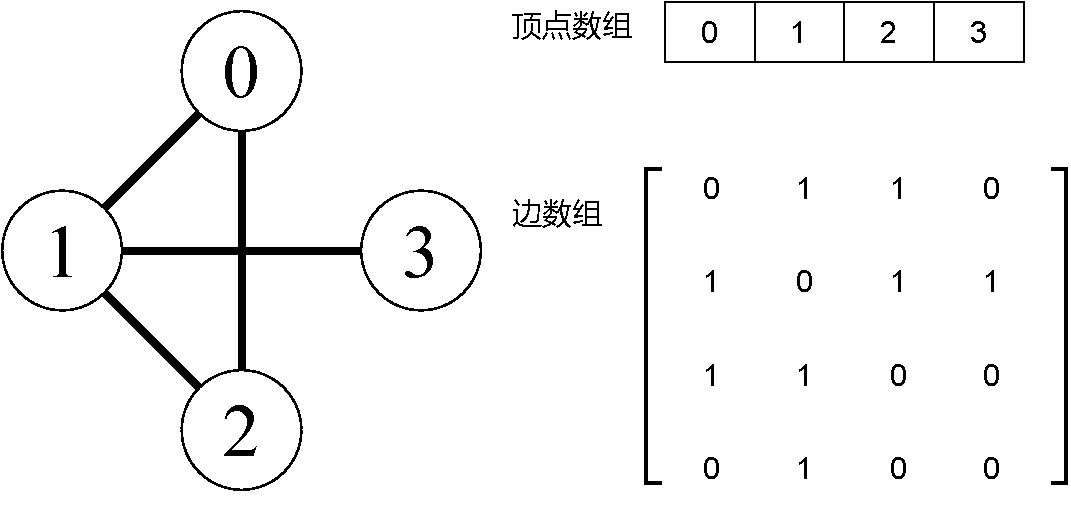
\includegraphics[width=7.3cm]{undirected_adj_mart.pdf}
        }
        \subfloat[有向图]{
            \label{pic:dir_adj_mart}
            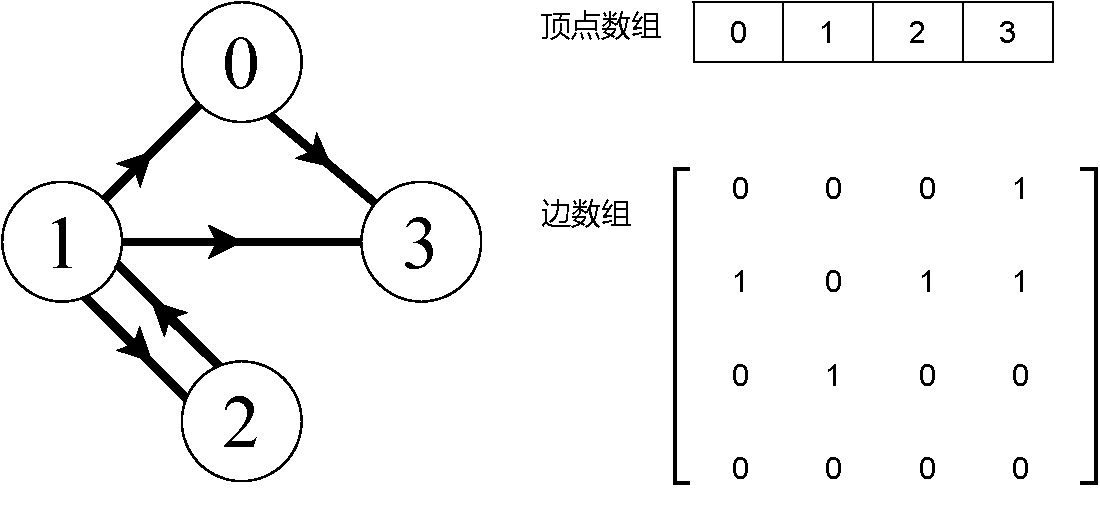
\includegraphics[width=6.41cm]{directed_adj_mart.pdf}
        }
        \caption{邻接矩阵}
        \label{fig:adj_mart}
    \end{figure}
    \item[(2)] 邻接表
    
        领接矩阵中即使两个顶点之间没有边,也会在矩阵中占据空间,对于边相对较少的稀疏图,使用邻接矩阵浪费很多存储空间。因此考虑对
    边使用链式存储的方式来避免空间浪费。领接表是由两部分组成。与邻接矩阵相同的是顶点也使用一维数组存储。而边信息不在使用二维数组,
    每个顶点的所有连接边存储为线性表,由于领接点的个数不定,采用单链表存储,无向图称为顶点的边表,有向图则称为顶点的出边表。

    \begin{figure}[h]
        \subfloat[无向图]{
            \label{pic:undir_adj_list}
            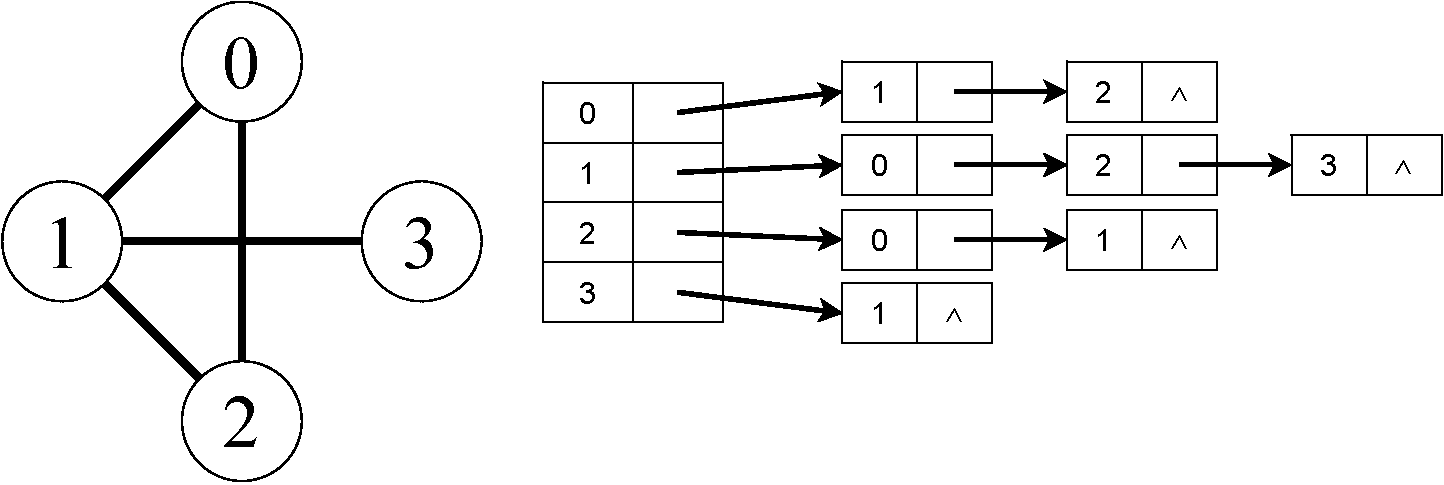
\includegraphics[width=.5\linewidth]{undirected_adj_list.pdf}
        }
        \subfloat[有向图]{
            \label{pic:dir_adj_list}
            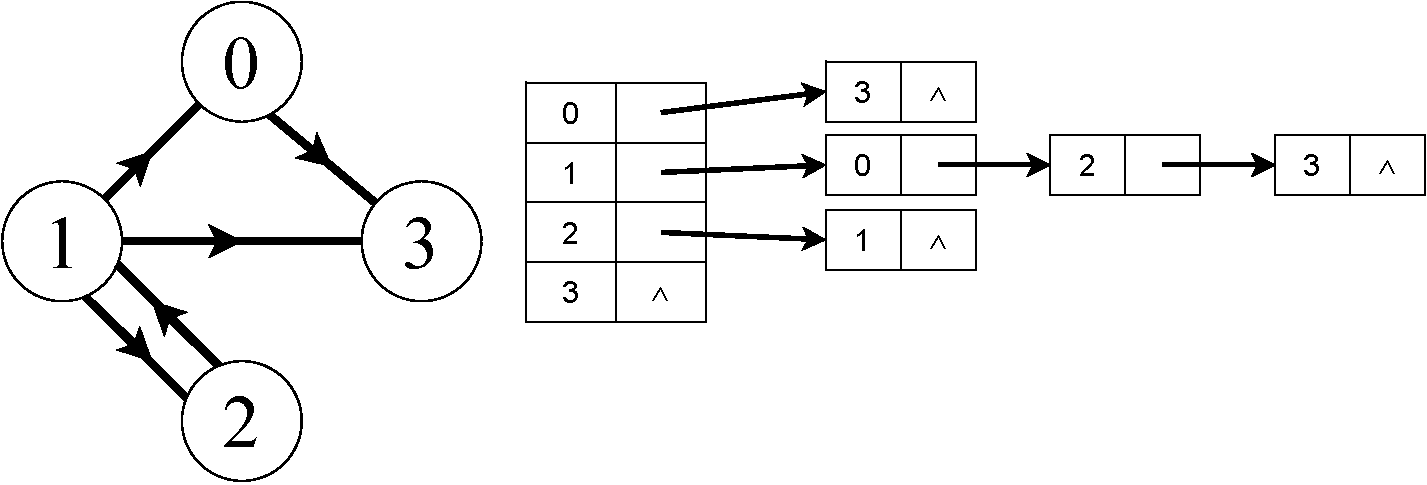
\includegraphics[width=.5\linewidth]{directed_adj_list.pdf}
        }
        \caption{邻接表}
        \label{fig:adj_list}
    \end{figure}
        
        在有向图中,每个顶点的出边表结点个数为该顶点的出度,若要求顶点的入度,则需遍历整个邻接表。有时为了便于求有向图中顶点的入度,
    会建立一个有向图的逆邻接表。逆邻接表与邻接表相反,每个顶点建立一个入边表。
    
    \item[(3)] 十字链表
    
        邻接表的缺陷是想要获取某个顶点入度需要遍历整个图,虽然可以通过再建立一个逆邻接表来弥补,但这样会带来更多的冗余存储消耗。十字链表
    将二者整合在一起解决这个问题。十字链表能够方便地求得顶点的出度和入度。而且创建十字链表的时间复杂度和邻接表相同。因此有向图使用十字链
    表存储是常见方法。

    \begin{figure}[h]
        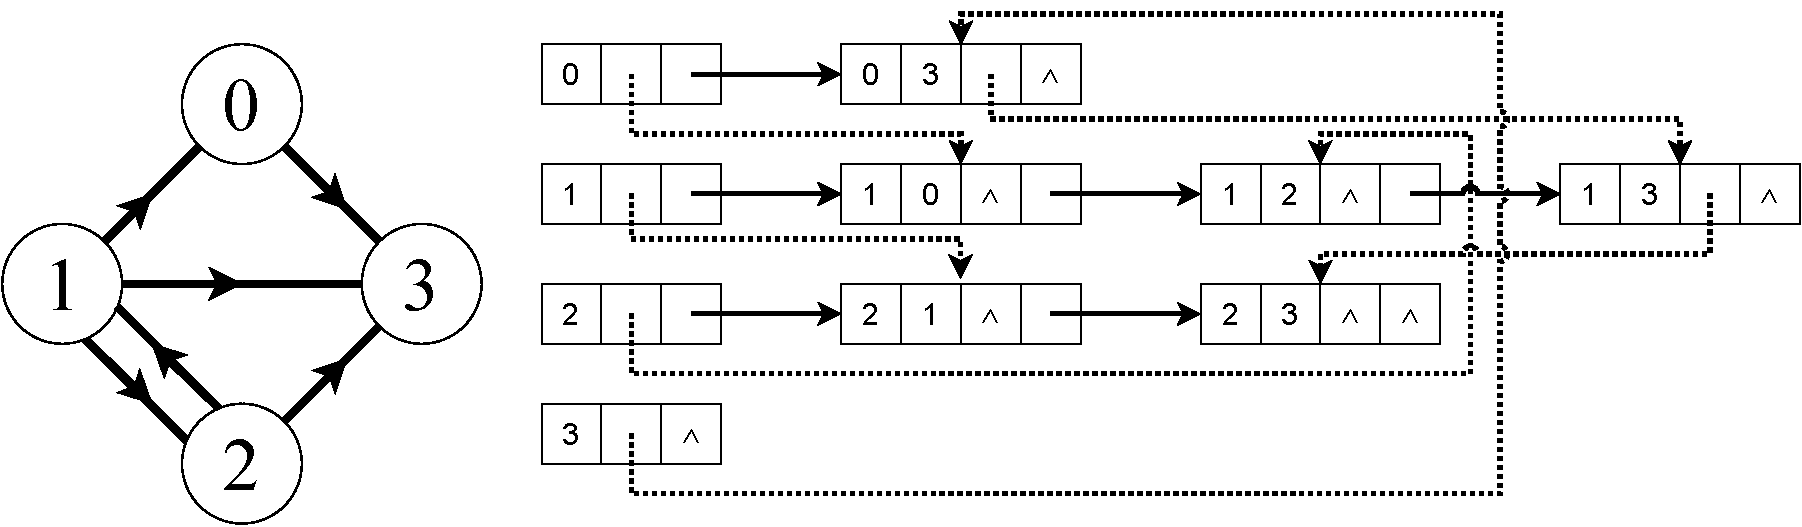
\includegraphics[width=\linewidth]{directed_orthogonal_list.pdf}
        \caption{十字链表}
        \label{fig:orthogonal_list}
    \end{figure}

    \item[(4)] 边集数组
        边集数组将每个条边的起点下标、终点下标和属性存储为顺序数组,其中属性可以为空。边集数组是以边为核心的存储结构,在边集数组中要查找一个顶点的度需要
    扫描整个边数组。它更适合对边依次进行处理的操作,而不适合针对顶点的操作。
    
    \begin{figure}[h]
        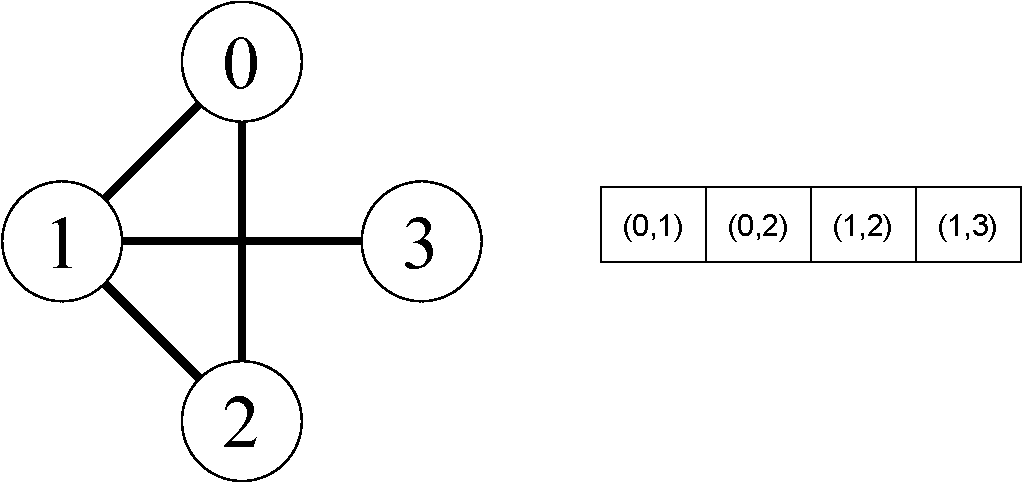
\includegraphics[width=\linewidth]{edges_array.pdf}
        \caption{边集数组}
        \label{fig:edges_array}
    \end{figure}

\end{enumerate}

\subsection{图的常用算法}
    图的算法提供了最有效的分析图数据结构的方法,它们描述了如何处理图以发现一些定性或者定量的结论。
图算法基于图论,利用顶点之间的关系来推断复杂系统的结构和变化。
\begin{enumerate}
    \item[(1)] 图的遍历
    图的遍历是指从图中的某一个顶点出发,按照某种搜索方法沿着图中的边对图中的所有顶点访问一次且仅访问一次。
按照访问顶点的顺序主要分为两类:广度优先搜索和深度优先搜索。广度优先搜索是一种分层的访问过程,从起始顶点出发
优先访问起始顶点的所有邻域,再访问邻域顶点的邻域,以此类推直到访问所有顶点。深度优先搜索选择访问过的顶点的任
意邻域顶点,尽可能的沿着边进行访问,直到不能继续前进则回溯。
    
    \item[(2)] 最短路径
    最短路径是在两个顶点之间寻找最短的路径,主要算法有Dijkstra算法、Floyd-Warshall算法。Dijkstra算法解决
单源最短路径,求解给定顶点到任意其他顶点间的最短路径。该算法根据最短路径的最优子结构性质,从起点开始不断更新
每个顶点到起点的最短路径,遍历完毕后可得起点到每个顶点得最短路径。Floyd-Warshall算法解决任意两点间的最短路
径,如果从一个点到另一个点的直接路径不是最短的,那最短路肯定要经过第三个点。所以就用所有的点都当一次中间点
插入到当前两点间最短路径中,来判断是不是任意两点之间经过中间点路程会减小。

    \item[(3)] 最小生成树
    最小生成树是在加权连通图里搜索边子集所构成的树,该树包括了图里的所有顶点,且其所有边的权值之和为最小。
主要有Prim算法、Kruskal算法。Prim算法维护一个顶点集和一个边集,顶点集任意加入一个图中顶点作为初始值,边集初始
为空,然后不断选择图中权值最小且其中一端在顶点集中的边,将边加入边集,将另一端加入顶点集。直到顶点集包含图中所有
顶点。Kruskal算法把所有的边按照权值先从小到大排列,接着按照顺序选取每条边,如果这条边的两个端点不属于同一集合,
那么就将它们合并,直到所有的点都属于同一个集合为止。

\end{enumerate}

\subsection{图数据的应用领域}
\label{subsec:graph-app}


    图数据能够建模多种领域的数据。很多问题能在图论支撑下借助图相关的算法得到高效解决,例如图形着色,网络路由,网络流等
。研究图计算高效处理大规模图数据,能推动社交网络分析、语义web分析、生物信息网络分析、自然语言处理和MLDM等新兴应用领域
的发展。此外图计算的应用领域还包括:流量图,用来监控和应对道路事故,分析网络安全,网页搜索[3];生物图,进行研究药物模
型(例如蛋白质相互作用),预测疾病爆发;社交图,对舆情分析,推荐人或产品和信息流跟踪等。

\begin{table}
   \begin{tabular}{|c|c|c|l|}
    \hline
    数据 & 顶点 & 边 & 典型问题\\
    \hline
    蛋白质结构网络 & 氨基酸 & 接触残基 & \makecell[l]{氨基酸模块化结构发现、\\蛋白质互相作用~\cite{Spontaneous}}\\
    \hline
    社交网络 &用户个体 & 关注关系 & 社会角色划分、好友推荐、圈子探测~\cite{Role} \\
    \hline
    Web连接结构 &Web页面&页面之间的超链接 & PageRank页面排名~\cite{PageRank}\\
    \hline
    软件网络& 计算节点& 计算节点之间的互联 & 软件调用规划~\cite{SoftwareHomology}\\
    \hline
   \end{tabular} 
   \caption{图数据的典型应用}
   \label{tab:graph-app}

\end{table}

    从表\ref{tab:graph-app}中可以看出图数据的运用领域广泛。在这些领域中,有很多值得探究的具体问题:如在生物信息学中,将氨基酸建模为顶点
将接触残基建模为边,形成蛋白质结构网络,使用频繁子图挖掘可以从中发现大量出现的氨基酸模块化结构。又如在社交网络中,
用户看作顶点用户之间建立的关系看作边,可以通过大度数顶点寻找权威,通过最短路径长度可以获知两个用户之间人脉距离。
上述问题中除了需要处理实体携带的信息,更多地需要从图的拓扑结构进行分析。这反映了图数据不同于其他数据的一个
特点:在图数据中的“关系”至关重要,不仅仅是顶点或者边的属性能够表达信息,图的拓扑结构本身也蕴含着知识。图挖掘的目的正是
为了从图数据结构中发现知识。

\section{图挖掘技术}
\label{sec:graph-mining}

    图挖掘是从海量的图模型数据中发现和提起有用知识和信息的过程。图数据注重事物之间的联系,图的结构体现了这种联系的总体
特征。研究者常用集聚系数、三角数量、闭合三角比值等等指标来衡量一个图数据集。这些指标的获得需要在图数据集中寻找一些特定
的子结构,如三角形、团、路径等等。发现这些子结构的过程称为模式挖掘,这些子结构被称为模式。

\begin{table}
    \label{tab:graph-parameter}
   \caption{图数据集的典型指标}
   \begin{tabular}{|c|l|}
    \hline
    指标 & 含义\\
    \hline
    集聚系数 &  \makecell[l]{每个顶点连接的邻域顶点之间边的数量,\\除以这些顶点之间可以连出的最大边数(即团)} \\
    \hline
    社交网络 & 三角形数量 \\
    \hline
    闭合三角比值 & 三角形的数量与所有连通三点组(即三角形和三顶点路径)的总量之比\\
    \hline
   \end{tabular} 
\end{table}

    模式挖掘是一个经典的图挖掘问题,被认为是研究最多的问题之一。图模式挖掘问题针对的是标记了顶点和边的输入图。模式是一
个任意的图结构,模式挖掘算法旨在发现输入他中所有模式与匹配的子图。如下:

    \textbf{图同构}:如果两个图$G$和$H$的顶点和边之间存在一对一映射,则称$G$和$H$同构,在有向图中边还需要保持方向的一致。
更非正式地说,如果忽略单个顶点之间的区别,同构指的是两个图具有相同边结构和相同拓扑。
    
    \textbf{子图}:$G$的子图$G'$有$V(G') \subseteq V(G), E(G') \subseteq E(G)$。子图中的每个节点也是父图中的一个节点,
子图中的每条边都是父图中的一条边。另外,当$G'$满足$\forall (u,v) \in E(G') \leftrightarrow (u,v) \in E(G)$时,称$G'$为
诱导子图。即$E(G')$包含了$E(G)$中所有两端连接在$V(G')$的边。

    \textbf{匹配和频率}:匹配指的是给定一个模式$P$,图$G$中能够找出子图$G'$与$P$同构。$P$在$G$中的频率是不同的$G'$的数量,
如果两个匹配不共享所有节点和边,则认为它们是不同的。
    
    模式挖掘集中在枚举满足用户指定特征的所有模式$P$的上。在输入数据集$G$上列出给定的模式$P$的子图,这些子图也称为$P$在$G$中
的嵌入。然后通过评估筛选出满足条件的模式,比如出现次数大于给定阈值。

    典型的模式挖掘应用包括以下几类:
\begin{enumerate}
    \item[(1)] 子图查询
    
    给定两个图$G$和$P$,确定$G$中是否包含与$P$同构的子图,也可以更简单地看作计算$H$出现次数是否大于零。
对于一般图,这是一个已知的NP完全问题。这项任务与图同构问题密切相关~\cite{Isomorphism},许多子图查询方法依赖于找到$G$中所有包含的子图,
然后检查找到的子图是否与$H$同构。一些子图查询算法使用了著名的nauty工具~\cite{Nauty}来辨别子图的类型~\cite{Towards,GTries,FANMOD}。

    \item[(2] 网络主题挖掘
        
    如果有某种子图,在图$G$中在出现次数高于其在随机图$R$中出现次数,则称为主题~\cite{Motifs},网络主题用于发现图数据中的局部规律。
常用的随机图$R$与图$G$保持相同度序列,通过多次随机交换$R$中的任意两条边其中一个顶点来实现,这样保持了度数不变。重要度来表现一个主题是否
经常出现的指标,对于每一个主题计算图$G$中主题个数$N_i^{real}$和随机图中主题个数$N_i^{rand}$,可得Z=score统计量
$Z_i\frac{N_i^{real}-N_i^{rand}}{N_i^{real}}$,标准化后得到重要度指标(significance profile)$SP_i=\frac{Z_i}{\sum_{k=1}^{n}Z_j}$
可以用来比较不同的主题相对重要程度。

    \item[(3)] 频繁子图挖掘

    找到在图$G$出现频率高于给定阈值的所有子图结构,最终根据频率对子图结构进行排序。与主题不同,频繁子图挖掘
不需要比较随机图,直接在图$G$中搜索。通常频繁子图挖掘问题有两种分支:输入一组图数据集在其中寻找其中大量共同出现的子图;
输入单个大的图数据搜索其中频率较高的子图~\cite{SurveyFSM}。主要方法是从最简单的模式(例如,一个顶点或一条边)开始在$G$中统计出现个数,
筛选掉频率小于$K$的模式。然后,通过再添加一个顶点或边来扩展模式,并重复统计个数然后筛选的步骤,候选集为空。这里运用了向下封闭属性进行剪枝,
即一个模式出现频率如果大于$K$,该模式的子图频率也一定大于$K$。

\end{enumerate}

    在模式挖掘中,子图同构是基础,网络主题挖掘、频繁子图挖掘更进一步要求统计同构发生的次数,模式计数算法正是其中的重点。子图同构本身就是
一项NP完全任务,想要再此基础上对寻找到的模式进行计数则更加困难。随着图数据集规模日趋庞大,顶点和边数量大于$10^9$的图数据愈来愈普遍,精确
计算模式出现次数的开销越来越难以接受,因此很多研究寻求使用近似计算理论来进行模式挖掘。下一章将介绍近似计算相关理论。

\section{近似计算技术}
\label{sec:approximate}
    
    目前广泛应用大数据处理框架主要作用是大规模数据分析,以批处理计算为主,其实时性需求得不到满足。在大数据应用场景下,数据价值会随着
时间的流逝而衰减,因此期望能够尽快对最新的数据做出分析并给出结果,并实时展示,以达到实时计算。但随着数据规模的日益庞大,计算数据的时
间却变得越来越长。为了缓解这个矛盾,提出了近似计算技术,它基于直观的考虑:在执行精确计算需要大量的计算资源,允许选择性的近似处理,达成
可以接受的精度损失和大规模的计算时间节约。有效的近似技术需要明智的选择近似策略,否则可能导致难以接受的质量损失。

\subsection{数据采样}
\label{subsec:sample}
    近似计算最常用的手段是是对查询或算法处理的输入进行采样。给定一个数据集(有时称之为“总体”),首先从数据集中随机选择少量元素。
然后对样本计算一些统计数据,例如样本、均值和方差。最后,这些统计信息用于估计查询结果的值,并提供估计精度的界限。
数据采样通过缩减数据集规模达到减少执行时间的效果,并且采样方法可以指定执行时间限制,通过预测在限制时间内处理能力来决定
样本的大小。
    
\subsubsection{数学模型}
\label{subsubsec:math-model}
    样本是通过某种随机过程从原始数据集中选择的一组元素,采样过程可按以下方式进行建模。用$t_j$表示数据集中的第$j$个元素
,用$X_j$表示样本中第$j$个元素出现次数的随机变量。$X_j$的样本空间是非负整数,即$X_j = \{x_j \ge 0\}$。不同的$X_j$取值
表示了不同的采样行为,比如$x_j = 0$表示$t_j$没有被采样到,否则$t_j$被采样到$x_j$次。通过改变采样过程(有替换、无替换、有偏差、
无偏差等),可以改变了各种$X_j$的统计特性,也改变了采样过程的统计特性。例如,在伯努利采样中,$t_j$采样概率为$p$,
样本空间为$X_j = \{0, 1\}$,即$P(X_j = 1) = p, P(X_j = 0) = 1-p$。
    将$X_j$和$t_j$应用于近似问题,需要构造可以用来估计近似结果的估计量。估计量$Y$可以看作一个函数$F$,将所有控制采样过程的随机
变量和所有数据元素参数化:
\begin{equation*}
    Y=F((t_1,X_1), (t_2,X_2),\ldots,(t_n,X_n))
\end{equation*}
通常$X_j = 0$的项表示没有被采样可以忽略:
\begin{equation*}
    \begin{aligned}
    Y&=F(\ldots,(t_{i-1},X_{i-1}), (t_i,0),(t_{i+1},X_{i+1}),\ldots)
    &=F(\ldots,(t_{i-1},X_{i-1}),(t_{i+1},X_{i+1}),\ldots)
    \end{aligned}
\end{equation*}
    $Y$是一个由函数$F$生成的新随机变量。通过对这个随机变量进行试验(即,执行采样过程以获得每个$x_j$,然后对结果应用$F$),可以
得到近似计算的估计值。

\subsubsection{估计质量}
\label{subsubsec:quality}
    通常采样方法用$Y$的偏差$bias(Y)$和方差$\sigma^2(Y)$来量化效用和准确性。
\begin{equation*}
    bias(Y)= E[Y]-Q
\end{equation*}
其中$E[Y]$是$Y$的预期值,$Q$是精确计算结果。偏差表示了$Y$平均值与$Q$的距离。当$bias(Y)=0$,称$Y$是$Q$的无偏估计。
\begin{equation*}
    \sigma^2(Y)= E[(Y - E[Y])^2]= E[Y^2] - E^2[Y]
\end{equation*}
方差表示Y围绕其平均值的差距,意味着估计量的可变程度。如果$Y$拥有较低的偏差和方差,则认为$Y$由较高的估计质量。

    所以很多用户还要求在给出估计结果的同时提供置信区间,通常表述为:“精确计算结果在$[l,h]$区间范围内的概率为$p$”。

    \textbf{中心极限定理}。中心极限定理表明对于独立的随机变量,即使变量本身不是正态分布,其归一化和的极限趋向于
正态分布。在数据采样中随着从分布中提取的独立样本数量接近无穷大,观察到的分布均值和样本均值之间的差异越来越接近正态分布。
对于$Y$有:
\begin{equation*}
    \lim_{n\rightarrow\infty}Y= N(E[Y], \sigma^2(Y))
\end{equation*}
当$Y$是$Q$的无偏估计时,可以假设估计误差也是正态分布:
\begin{equation*}
    Q-Y \approx N(0, \sigma^2(Y))
\end{equation*}
选择不同的置信度,可以确定置信区间的两个端点$lo$和$hi$:
\begin{equation*}
    p=\int_{lo}^{hi}f_N(x)dx
\end{equation*}
其中$f_N$是$N(0, \sigma^2(Y))$的概率密度函数,这个式子表示$lo \le Q-Y \le hi$的概率为$p$。令$l=lo+Y$、$h=hi+Y$,
则$Q$在$[l,h]$区间范围内的概率为$p$。

    以置信度0.95为例,有:
\begin{equation*}
    \int_{-1.96\sigma(Y)}^{1.96\sigma(Y)}f_N(x)dx=0.95
\end{equation*}
则可以称$Q$在$[Y-1.96\sigma(Y), Y+1.96\sigma(Y)]$范围内的概率为95\%。

    根据统计理论,中心极限定理具有很大的普遍性,即便在样本数量不是非常庞大,假设$Y$误差服从正态分布依然是安全的。

    \textbf{切比雪夫界}。在数据采样的运用中,如果回避对于数据分布的假设,可以采用切比雪夫不等式,它相比中心极
限定理更宽松。对于无偏估计$Y$有:
\begin{equation*}
    Pr\left[\vert Q-Y \vert \ge p^{-\frac{1}{2}}\sigma(Y) \right] \le p
\end{equation*}
可以称Q在$\left[ Y-p^{-\frac{1}{2}}\sigma(Y), Y+p^{-\frac{1}{2}}\sigma(Y) \right]$区间内的概率为$p$。

    \textbf{霍夫丁界}。当$Y$的方差难以计算时,可以采用霍夫丁不等式来估计置信区间,它适用于$Y=\frac{1}{n}\sum_iX_i$
且$X_i$值有界的情况:
\begin{equation*}
    Pr\left[\vert Y-E[Y] \vert \ge d \right] \le 2exp\left(-\frac{2d^2n^2}{\sum_i(lo_i-hi_i)^2}\right)
\end{equation*}
其中$lo_i$和$hi_i$是每个$X_i$值域的上下界,实际运用中,常用所有$X_i$中的最大值$MAX(X_i)$最小值$MIN(X_i)$来近似
处理$\sum_i(lo_i-hi_i)^2 \approx n(MAX(X_i) - MIN(X_i))^2$。霍夫丁界通常更为宽松。

    \textbf{切尔诺夫界}。切尔诺夫界与霍夫丁界密切相关,适用于$Y=\frac{1}{n}\sum_iX_i$但$X_i$取值只为0或1的情况。
切尔诺夫界不直接构造基于采样的置信区间,但它们为各种采样方法构造了精度证明的重要工具。


\subsubsection{对歪斜数据的采样方法}
\label{subsubsec:advantages-drawbacks}
    数据采样是一种简洁的近似计算的手段,从概念上很容易理解从数据集中随机选择元素的思路,然后在样本上放大计算结果以猜测
整个数据集的结果。但均匀随机地数据采样往往对有歪斜的数据集比较敏感,数量稀少而又包含异常值的数据元素可能会导致估计结果
质量较差。通常使用措施来处理歪斜数据。

    \textbf{分层采样法}。将总体数据集分类成不同类型的子集(这些子集被称为层),按照各层与总体数量之间的比例从不同的层中
进行采样。相对于均匀随机采样,分层采样通过划分层,使得采样的数据更具有代表性,它更适合不同类型数据数量相差较大的数据集。
分层采样往往需要对数据集有一定的先验知识,预先了解数据构成,才能有效的对数据集进行分类。

    \textbf{生成概要}。数据采样是在计算开始后构造样本而不需要提前生成,因此具有灵活性,可以实时地根据选取样本的多寡来权衡
精度和执行时间。而对数据集进行预先分析,提取数据集关键属性建立某种的数据结构,这种数据结构被称为概要。生成概要需要在
采样计算开始前对数据集进行遍历、统计,带来一定的额外开销,但合理的概要能够对数据采样起到很多帮助。如直方图按照数据间隔划分
桶,统计桶中的样本数量,是一种按照数据值的数量级来分类的结构,可以直接用于分层采样法。

\section{图近似模式挖掘技术}
\label{sec:graph-approximate}
    近似计算技术是大数据分析中取得很多成功的方法,因此很多研究探索在图模式挖掘中运用类似的技术。与其他领域中近似
计算相同,近似模式挖掘也主要使用数据采样策略,其主要思想是将图中的边建模为流并从中采样模式的实例,然后使用采样
概率来估计模式出现次数。研究者提出了多种基于不同的采样方法的模式挖掘技术。

\subsection{基于均匀采样的模式挖掘}
\label{subsec:uniform}
    均匀采样是对图数据边流$S$中的每一条边进行固定概率$p$的采样,本质是概率为$p$的$n$重伯努利实验,其中$n=|S|$。
当一条边$e(u, v) \in S$被采样到后,将$e$存储到$E_{samp}$。然后在$E_{samp}$执行精确模式挖掘算法,以三角形计数
为例。在$E_{samp}$中查找$N_{uv}=N_u \cap N_v$,$N_u$和$N_v$分别是顶点$u$和顶点$v$的邻接顶点集,$N_{uv}$
是$N_u$和$N_v$的交集,$N_{uv}$中每一个顶点都能够和边$e(u, v)$组成新的三角形。因此$e$加入到$E_{samp}$后,新
增三角形个数为$|N_{uv}|$。因为三角形中每一条边被采样到的概率为$p$,所以直观的认为三角形被采样到的概率应
为$p^3$,新增的估计三角形数量应为$|N_{uv}|*\frac{1}{p^3}$。当边流$S$中所有边遍历完毕后,可得出最终的估算结果。

\begin{figure}
	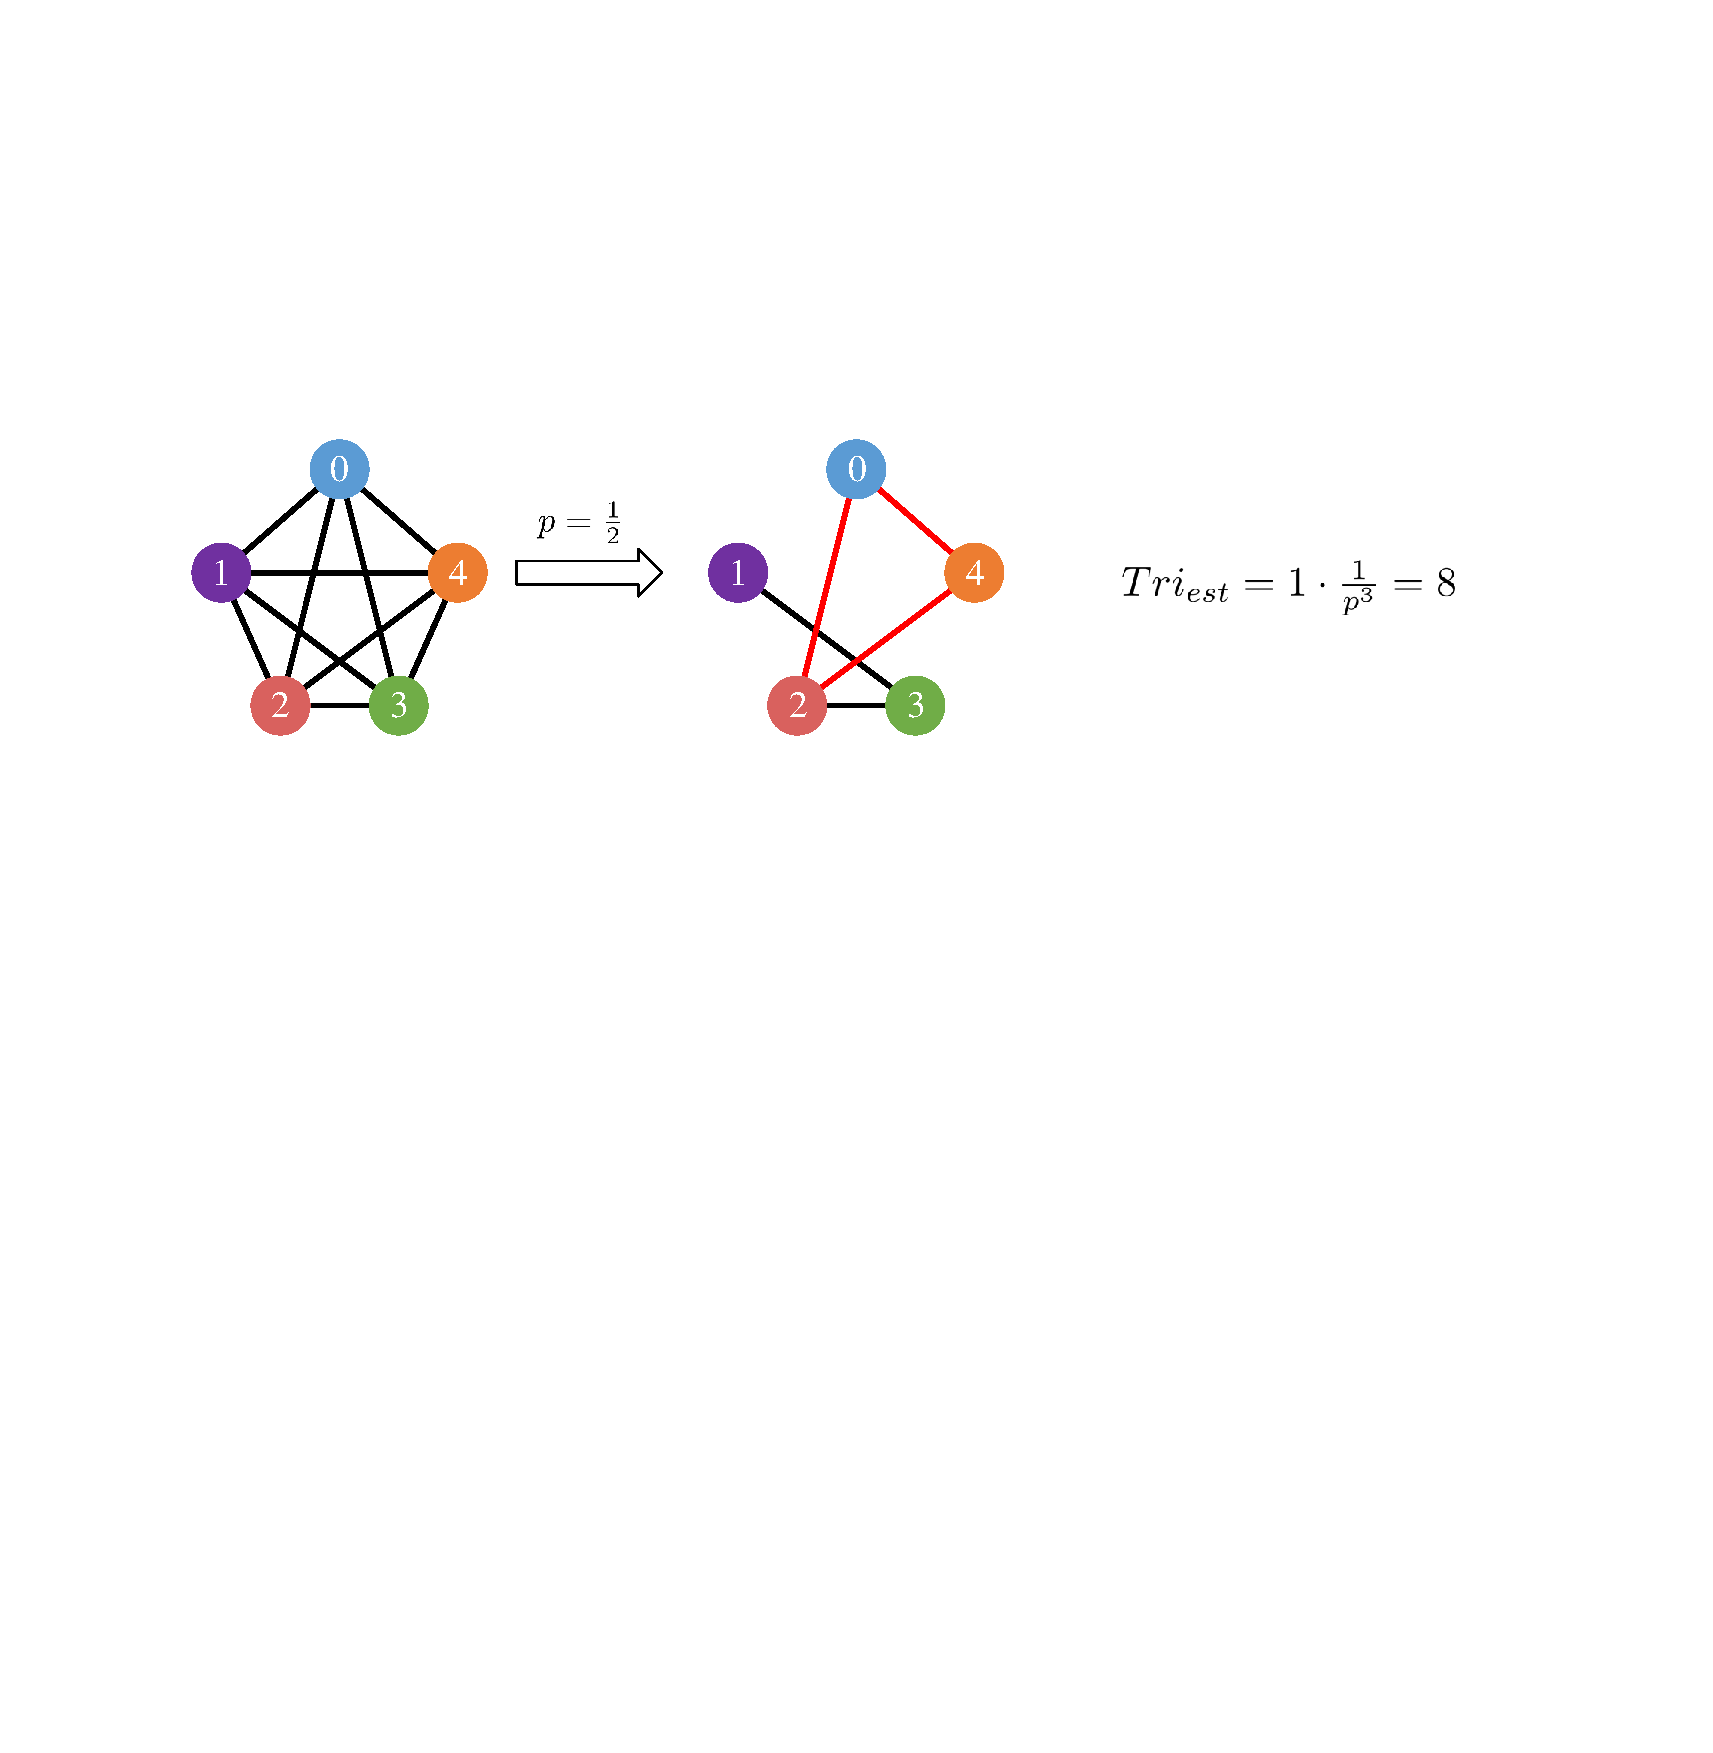
\includegraphics[width=\linewidth]{uniform.pdf}
	\caption{均匀采样示例}
	\label{fig:uniform}
\end{figure}
     如图~\ref{fig:uniform}所示,在图$G$中以$\frac{1}{2}$概率均匀采样,在采样边$E_{samp}$中发现一个三角形,根据采样
概率估算形三角数量为8个。

\subsection{基于库采样的模式挖掘}
\label{subsec:reservoir}
    上一节\ref{subsec:uniform}中描述的均匀采样完整地存储所有被采样的边,当边的数量很大时,采样边的存储开销也会变得很大
,因此提出了库采样。库采样技术是通过限制样本规模来控制采样过程中的存储开销。下面给出一种基础方法的描述。

    在扫描图边流$S$中维护一个固定容量为$M$的库$E_{samp}$,访问在边流中第$i$条边$e_i$时,如果$i<=M$无条件地将边存储到库中,
而当$i>M$后以概率$\frac{M}{i}$进行采样如果$e_i$被采样到则随机替换掉库中一条边。这种采样方法可以看作在$i$条边中均匀地选
择$M$条边。每条边加入库中执行模式挖掘得出更新模式计数$\tau$,具体方法与\ref{subsec:uniform}中描述的过程类似,不同之处在于需要
挖掘出被替换掉关联的模式并从计数中减去对应数量。接着根据$\tau$估算原图中模式总数。

    挖掘的模式$p$的边数为$k$。当$i<M$,所有边都被存储到了$E_{samp}$中此时$\tau$为准确计数。当$k>MIN(i,M)$,$p$不可能被计数。
所以重点是当$k<M<i$时的$p$被计数的概率。设:
\begin{itemize}
    \item $I$是原图中任意一个与$p$同构的子图,$E_I$是$I$的边集且$E_I \subseteq S$。
    \item $\alpha$是边集的集合,$\alpha$中每个元素大小为$M$且包含$E_I$,$\alpha={A: |A| = M , E_I \subseteq A}$。
\end{itemize}
则有:
\begin{equation*}
    |\alpha|=\left(\begin{array}{c}
        i-k\\
        M-k
    \end{array}\right)
\end{equation*}
又对于任意一个大小为$M$的边集$A$,被采样到库中的概率为:
\begin{equation*}
    Pr(E_{samp}=A)=\left(\begin{array}{c}
        i\\
        M
    \end{array}\right)
\end{equation*}
$E_I$出现在$E_{samp}$中的概率:
\begin{equation*}
    \begin{aligned}
        Pr(E_I \subseteq E_{samp})&=Pr(E_{samp} \in \alpha)=\sum_{A\in\alpha}Pr(E_{samp}=A)\\
        &=\frac{\left(\begin{array}{c} i-k \\ M-k \end{array}\right)}{\left(\begin{array}{c} i \\ M \end{array}\right)}
    \end{aligned}
\end{equation*}
因此对原图中模式总数估计为$\frac{\tau}{Pr(E_I \subseteq E_{samp})}$。
 
\subsection{基于邻域采样的模式挖掘}
\label{subsec:neighbor}
    邻域采样是利用模式的连通性提出的一种采样方法,首先在边集中对一条边采样,然后后续从已采样边的邻域中添加更多边,
直到边形成模式或者边流中不能再找出邻域。

    设图数据集的边流大小为$m$,模式$p$的边数为$k$。从图中以概率$Pr(l_0)=\frac{1}{m}$采样第一条边$l_0$。在出现于$l_0$之后的
边流中搜索$l_0$的邻域$N(l_0)$,从中以概率$Pr(l_1)=\frac{1}{|N(l_0)|}$采样$l_1$。同样,在$l_1$后续边流中搜索$N(l_0) \cup N(l_1)$
并以概率$Pr(l_2)=\frac{1}{|N(l_0) \cup N(l_1)|}$采样$l_2$。以此类推,直到剩余最后一条边$l_{k-1}$,停止采样直接在剩余边流中检查是否存在
$l_{k-1}$能够与之前采样的边形成$p$的同构子图。如果是以$\frac{1}{Pr(l_0)*Pr(l_1)*\cdots*Pr(l_{k-2})}$估计原图中模式数量,否则估计为0。
邻域采样方法对边流执行一次上述过程称为运行了一个估计器,最终结果是多个估计器结果的均值。

\begin{figure}
    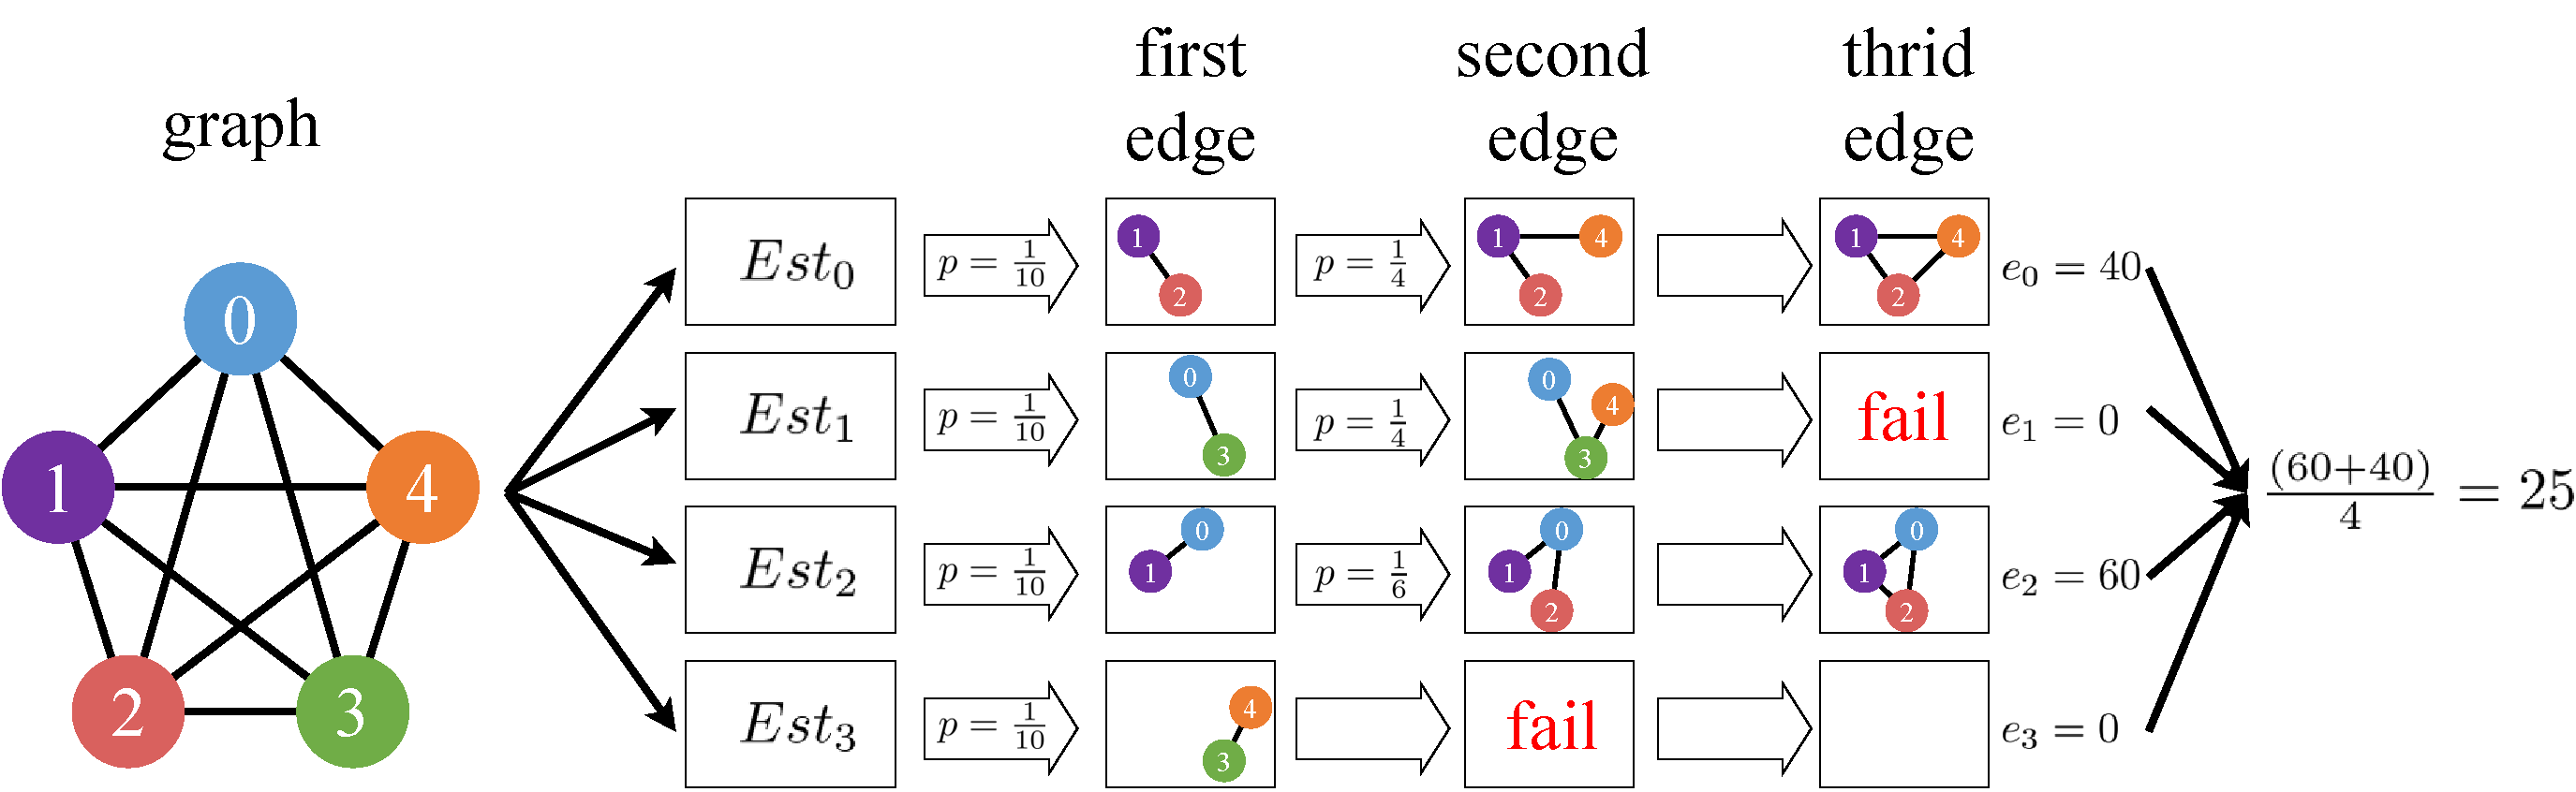
\includegraphics[width=\linewidth]{tri_nei_samp.pdf}
	\caption{基于邻域采样的三角形计数示例}
	\label{fig:tri_nei}
\end{figure}
    在图\ref{fig:tri_nei}中展示了如何使用邻域采样方法进行三角形计数,这里使用了四个估计器。以第一个估计器为例,首先以$\frac{1}{10}$的概率
采样了边$(1,2)$作为$l_0$,在后续边流中邻域$N(l_0)={(1,3),(1,4),(2,3),(2,4)}$,值得注意的是$(0,1),(0,2)$也是$l_0$的邻边,但由于在边流中
出现早于$l_0$并未被计入$l_0$的后续邻域。接着以$\frac{1}{4}$的概率采样$(1,4)$作为$l_1$,最后在$N(l_0) \cup N(l_1) = {(2,3),(2,4)}$中检
测到$(2,4)$可以形成三角形,因此输出估计值40。而在第二个估计器中,$l_1$采样到(3,4)后续已经没有邻域,因此输出估计值0。最后使用四个估计器的均
值作为最终结果。
    
    邻域采样相较于均匀采样和库采样,考虑模式的连通性,从已有边的邻域中继续采样边要比从所有边中采样概率大很多,因此提高了估计精度、加快了采
样速度。并且多个估计器相互独立,可以得益于并行化执行。但是邻域采样方法单一的估计器计算结果方差很大,对运行需要大量的估计器来保证估计精度。
本文的模式近似挖掘方法基于邻域采样方法,目的是根据图的幂律特征对邻域采样方法进行优化。

\section{幂律图理论}
\label{sec:pow-law-graph}
    近年来随着Web2.0、大数据、社交网络、机器学习和数据挖掘等技术的高速发展,很多领域抽象出来的图规模呈指数级增长。
图中边的数量可达到亿万级别,另外再加上自然图往往表现出非常倾斜的幂律分布特性,对图计算带来了巨大挑战。
    
    \textbf{幂律分布}。幂律分布也常被称为重尾分布、帕累托分布、Zipfian分布等,是计算机科学应用中越来越常见的模型;例如,它们已被用于描述
互联网图的文件大小分布和出度入度分布。下面描述幂律分布的一些基础定义:

    如果:
\begin{equation*}
    Pr(X \ge x) \sim cx^{-k}, c > 0, k > 0
\end{equation*}
非负随机变量X被称为具有幂律分布,幂律分布描述了分布的尾部根据指数$-k$下降的情况。概率密度函数为:
\begin{equation*}
    f(x) = cx^{-k-1}, c > 0, k > 0
\end{equation*}
幂律分布在双对数坐标下为一条直线,这为辨别是否具有幂律提供了一个简单的经验测试方法:
\begin{equation*}
    lnf(x) = lnc-rlnx, c > 0, r > 0
\end{equation*}
幂律分布的重要特性是无标度性,使得幂律分布的数据能够在任何规模下都能保持整体特性。
\begin{equation*}
    f(ax) = (ca^{-k-1})x^{-k-1}=bf(x)
\end{equation*}

    \textbf{幂律图}。是指图的度数$d$和具有该度数的顶点$v_{\#}(d)$满足关系
\begin{equation*}
    v_{\#}(d)=c \cdot d^{-k}
\end{equation*}
该式表示了幂律图有大量具有极低度的顶点和少数具有相对高度的顶点。由于幂律图分体现了无标度性,可以使用小规模数据集得出整体数据的特性。
而随机图通常顶点之间均匀的形成连接边,图\ref{fig:rand-vs-pow}展示随机图和幂律图的对比。

\begin{figure}
    \subfloat[随机图]{
        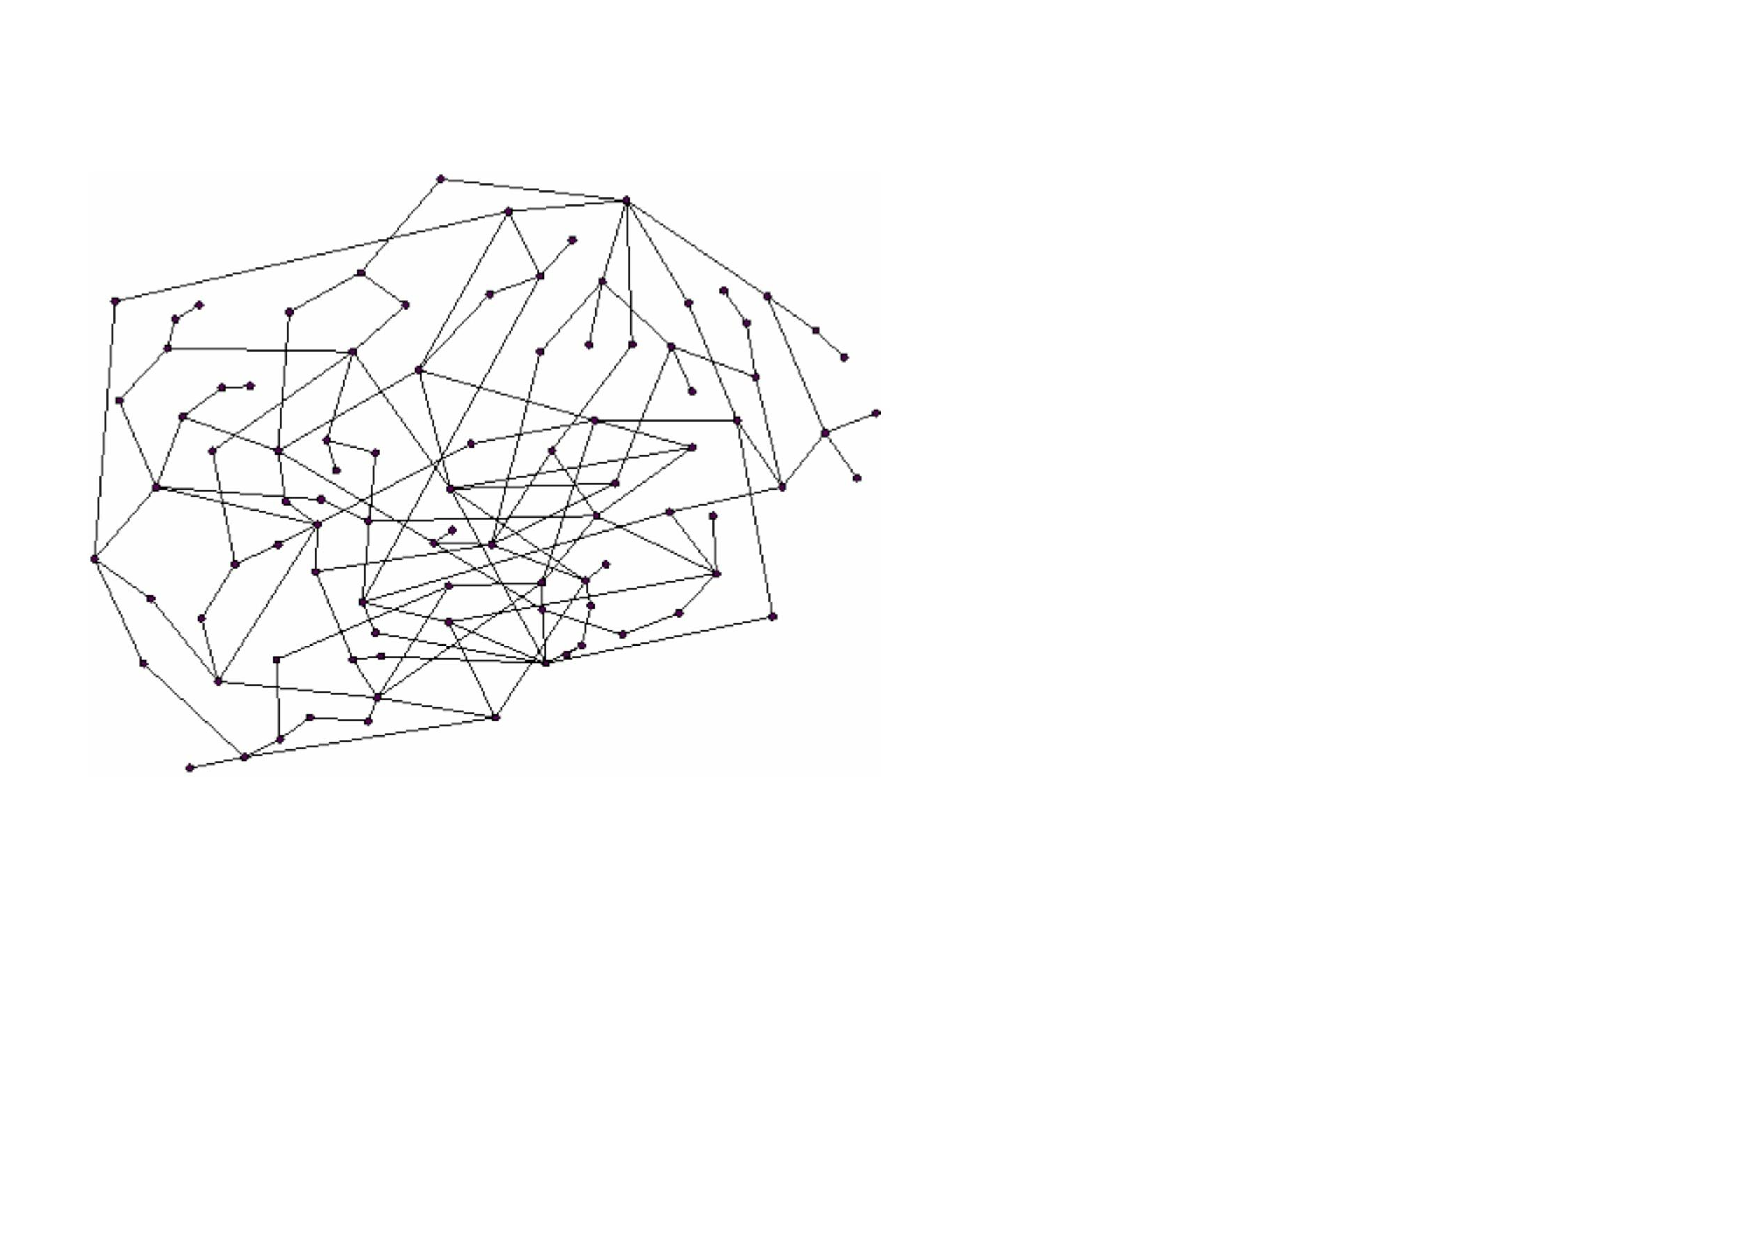
\includegraphics[width=.5\linewidth]{pic/graph-example/random_graph.pdf}
    }
    \subfloat[幂律图]{
        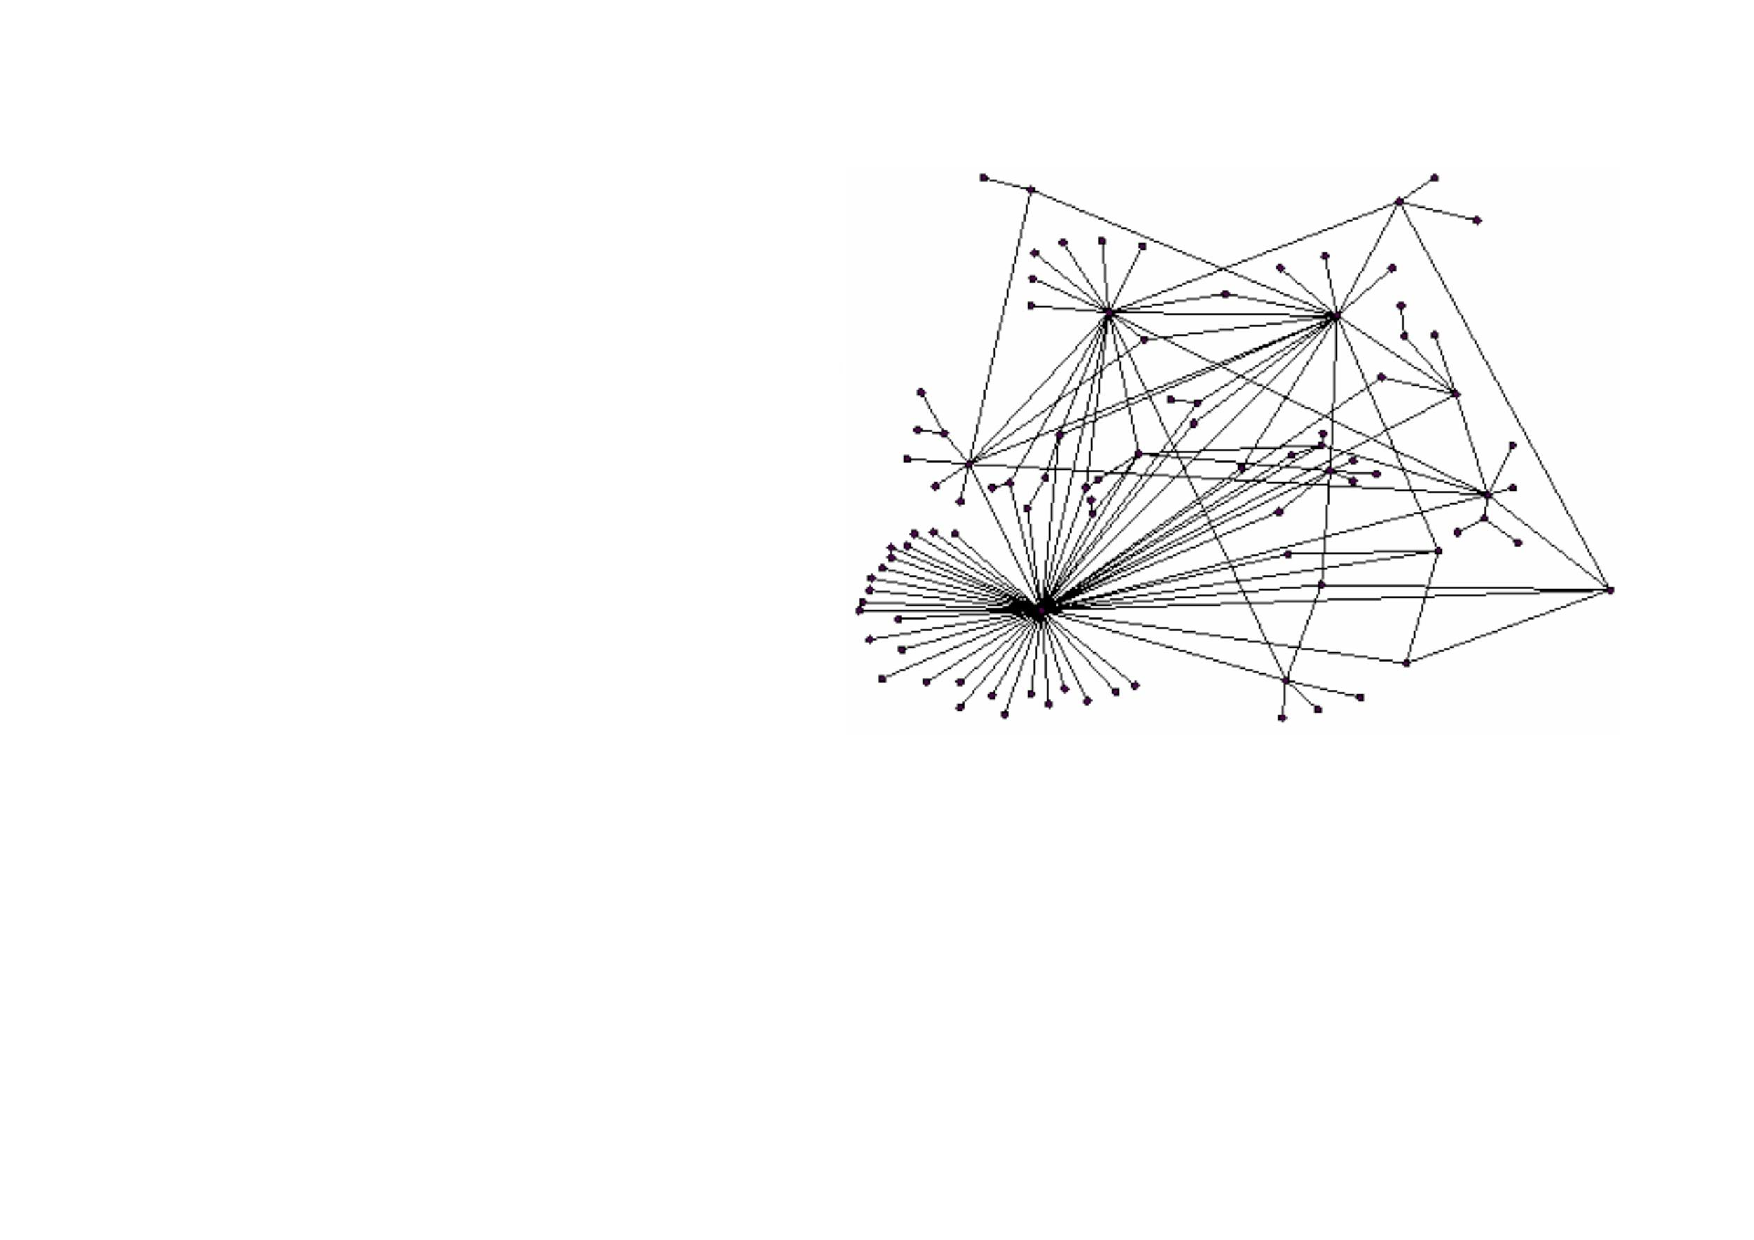
\includegraphics[width=.5\linewidth]{pic/graph-example/powerlaw-graph.pdf}
    }
    \caption{随机图和幂律图}
    \label{fig:rand-vs-pow}

\end{figure}

    真实世界中,幂律图主要构成原因是“优势优先”或“赢者通吃”现象,比如在社交媒体中人们往往倾向于关注已经有大量人气的用户,又如论文引用中
论文的新增引用往往和已有引用成正比。因此通常可以使用择优链接模型(Preferential attachment)来生成幂律图。顶点按顺序加入图中,当第$j$个顶点
加入时,连接到之前的顶点$i$的概率与$i$的度数$d_i$成正比。
\begin{equation*}
    P(j \rightarrow i)=\frac{d_i}{\sum_k d_k}
\end{equation*}
    如随着顶点的加入,形成满足度数满足幂律分布的图。

\begin{figure}
    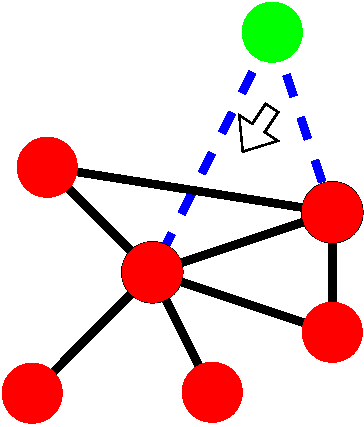
\includegraphics[width=.5\linewidth]{pic/gen_powlaw.pdf}
    \caption{择优链接模型形成幂律图}
    \label{fig:gen-pow}

\end{figure}

\section{回归分析}
\label{sec:regression-analysis}

    回归分析是分析数据的一种统计学方法,对两个或者多个变量之间的关系进行定量分析,通过建立起变量之间的特定函数模型,能够
通过某一个或某一组变量来预测需要变量的变化趋势。

    其中需要预测的变量被称为因变量(也称被解释变量、依变量),用于观察的变量称为自变量(也称解释变量、独立变量)。回归分析目的
在于找到最能够代表数据的一条曲线即函数关系式,用这条曲线表示因变量和自变量之间的关系。

    回归分析有以下变量:
\begin{itemize}
    \item $\beta$:一个或一组未知参数,它们是回归分析需要确定的目标。
    \item $X$:自变量
    \item $Y$:因变量
\end{itemize}
    
    回归分析需要一个函数式$f$将因变量$Y$与自变量$X$和未知参数$\beta$联系起来
\begin{equation*}
    Y = f(X,\beta)
\end{equation*}
$f$的基本形式需要预先指定,通常根据先验知识确定$f$的表达式,如果难以根据已有知识得出式子则需要选择一个广泛适合的$f$。

    在确定$f$之后,需要利用因变量$Y$和自变量$X$的真实数据来确定未知参数$\beta$的值。根据$\beta$数量$k$的不同,对数据量$N$有一定的要求:
\begin{itemize}
    \item 如果数据量$N<k$时大多数回归方法都难以得出$\beta$的确定解。
    \item 如果$N=k$且$f$是线性函数式,能够列出含有$k$个未知数和$k$个方程的方程组,则可以得出精确解。如果$f$为非线性函数式,则可能无解也可能多个解。
    \item 如果$N>k$,可以看作是求解关于$\beta$的超定方程,拥有足够的信息可以得出一个和数据最接近的$\beta$。回归分析的实际运用中通常遇到的是这种情况。
\end{itemize}

    依据$f$的函数类型,回归分析常分为线性回归分析和非线性回归分析。

    \textbf{线性回归}。线性回归中是因变量和自变量之间关系为线性模型,简单线性回归中常用的函数关系为
\begin{equation*}
    y = \beta_0+\beta_1x
\end{equation*}
其中$\beta_0$是直线在y轴的截距,$\beta_1$是直线的斜率。

    线性回归常用最小二乘法,通过最小化估计值和真实值之间差的平方和来求解$\beta$。
\begin{equation*}
    argmin\sum_{i=1}^{n}(y_i-\hat{y}_i)^2=\sum_{i=1}^{n}(y_i-\beta_0-\beta_1x_i)^2
\end{equation*}
最小二乘法得到如下解:
\begin{equation*}
    \left\{\begin{array}{l}
        \beta_1=\frac{n \sum_{i=1}^n x_i y_i-\left(\sum_{i=1}^n x_i\right)\left(\sum_{i=1}^n y_i\right)}{n \sum_{i=1}^n x_i^2-\left(\sum_{i=1}^n x_i\right)^2} \\
        \beta_0=y-\beta_1 x
        \end{array}\right.
\end{equation*}

    \textbf{非线性回归}。非线性回归是回归分析的一种方式。寻找因变量和自变量之间的函数模型,该函数是自变量和一组参数的非线性
组合,非线性值指的是变量指数不全为1。非线性回归常使用高斯-牛顿迭代法,在每次迭代中不断修正参数值使残差平方和达到最小
输入一组观测数据${(x_0,y_0),(x_1,y_1),\ldots,(x_{n-1},y_{n-1})}$,设置函数基本模型$f(c;x)$,其中$\mathbf{\beta}=(\beta_0,\beta_1,\beta_{p-1})^T$表示需要回归的参数。
设$\mathbf{g}^{(0)}=\left(g_0^{(0)},g_1^{(0)},\ldots,g_{p-1}^{(0)}\right)$是参数的初始值。对于任意$x_i$,将$f(x_i,\mathbf{\beta})$在$\mathbf{g}^{(0)}$处作一阶
泰勒展开:

\begin{equation*}
    f(x_i,\mathbf{\beta})=f(\mathbf{g}^{(0)};x_i) + \sum_{k=0}^{p-1}\left[\frac{\partial f(x_i,\mathbf{\beta})}{\partial \beta_k}\right]_{\mathbf{\beta}=\mathbf{g}^{(0)}}\left(\beta_k-g_k^{(0)}\right)
\end{equation*}
则有:
\begin{equation*}
    y_i - f(x_i,\mathbf{g}^{(0)}) \approx \sum_{k=0}^{p-1}\left[\frac{\partial f(x_i),\mathbf{\beta}}{\partial \beta_k}\right]_{\mathbf{\beta}=\mathbf{g}^{(0)}}\left(\beta_k-g_k^{(0)}\right)
\end{equation*}
令
\begin{equation*}
    y_i^{(0)}=y_i- f(x_i,\mathbf{g}^{(0)}), D_{i k}^{(0)}=\left[\frac{\partial f(x_i,\mathbf{\beta})}{\partial \beta_k}\right]_{\mathbf{\beta}=\mathbf{g}^{(0)}}, b_k^{(0)}=\beta_k-g_k^{(0)}
\end{equation*}
有
\begin{equation*}
    y_i^{(0)} \approx \sum_{k=0}^{p-1} D_{i k}^{(0)} b_k^{(0)}, \quad(i=1,2, \ldots, n)
\end{equation*}
以矩阵形式表示:
\begin{equation*}
    \mathbf{Y}^{(0)} \approx \mathbf{D}^{(0)} \mathbf{b}^{(0)}
\end{equation*}
其中
\begin{equation*}
    \mathbf{Y}_{n \times p}^{(0)}=\left[\begin{array}{c}
        y_1-f\left(g^{(0)};x_0\right) \\
        \cdots \\
        y_n-f\left(g^{(0)};x_{n-1}\right)
        \end{array}\right], \mathbf{D}_{n \times p}^{(0)}=\left[\begin{array}{ccc}
        D_{00}^{(0)} & \cdots & D_{0 p-1}^{(0)} \\
        \vdots & & \vdots \\
        D_{n-1 0}^{(0)} & \cdots & D_{n-1 p-1}^{(0)}
        \end{array}\right], \mathbf{b}_{p \times 1}^0=\left[\begin{array}{c}
        b_0^{(0)} \\
        \vdots \\
        b_{p-1}^{(0)}
        \end{array}\right]
\end{equation*}
用最小平方法估计修正$\mathbf{b}^{(0)}$,并更新$\mathbf{g}^{(0)}$
\begin{equation*}
    \begin{aligned}
        &\mathbf{b}^{(0)}=\left(\mathbf{D}^{(0) T} \mathbf{D}^{(0)}\right)^{-1} \mathbf{D}^{(0) T} \mathbf{Y}^{(0)} \\
        &\mathbf{g}^{(1)} =\mathbf{g}^{(0)}+\mathbf{b}^{(0)}
    \end{aligned}
\end{equation*}
每轮迭代中检验残差平方和
\begin{equation*}
    SSR^{(s)}=\sum_{i=0}^n\left[y_i-f\left( \mathbf{g}^{(s)};x_i\right)\right]^2
\end{equation*}
当满足给定的允许误差率$K$,即满足
\begin{equation*}
    \left|\frac{S S R^{(s)}-S S R^{(s-1)}}{S S R^{(s)}}\right| \leq K
\end{equation*}
停止迭代,输出$\mathbf{g}^{(s)}$。

\section{本章小结}
\label{sec:theroy-summary}
    在本章中首先描述了图数据的基础理论以及实际运用。接着介绍了图挖掘的相关技术,图挖掘正是从图数据中挖掘知识。
然后分析了近似计算的相关技术以及近似技术在图模式挖掘中的运用。最后介绍了图的幂律性质和相关的数学分析方法。


\chapter{系统分析与设计}

\section{图的幂律分布特性分析}
\label{sec:pow-law-analysis}

\begin{figure}
    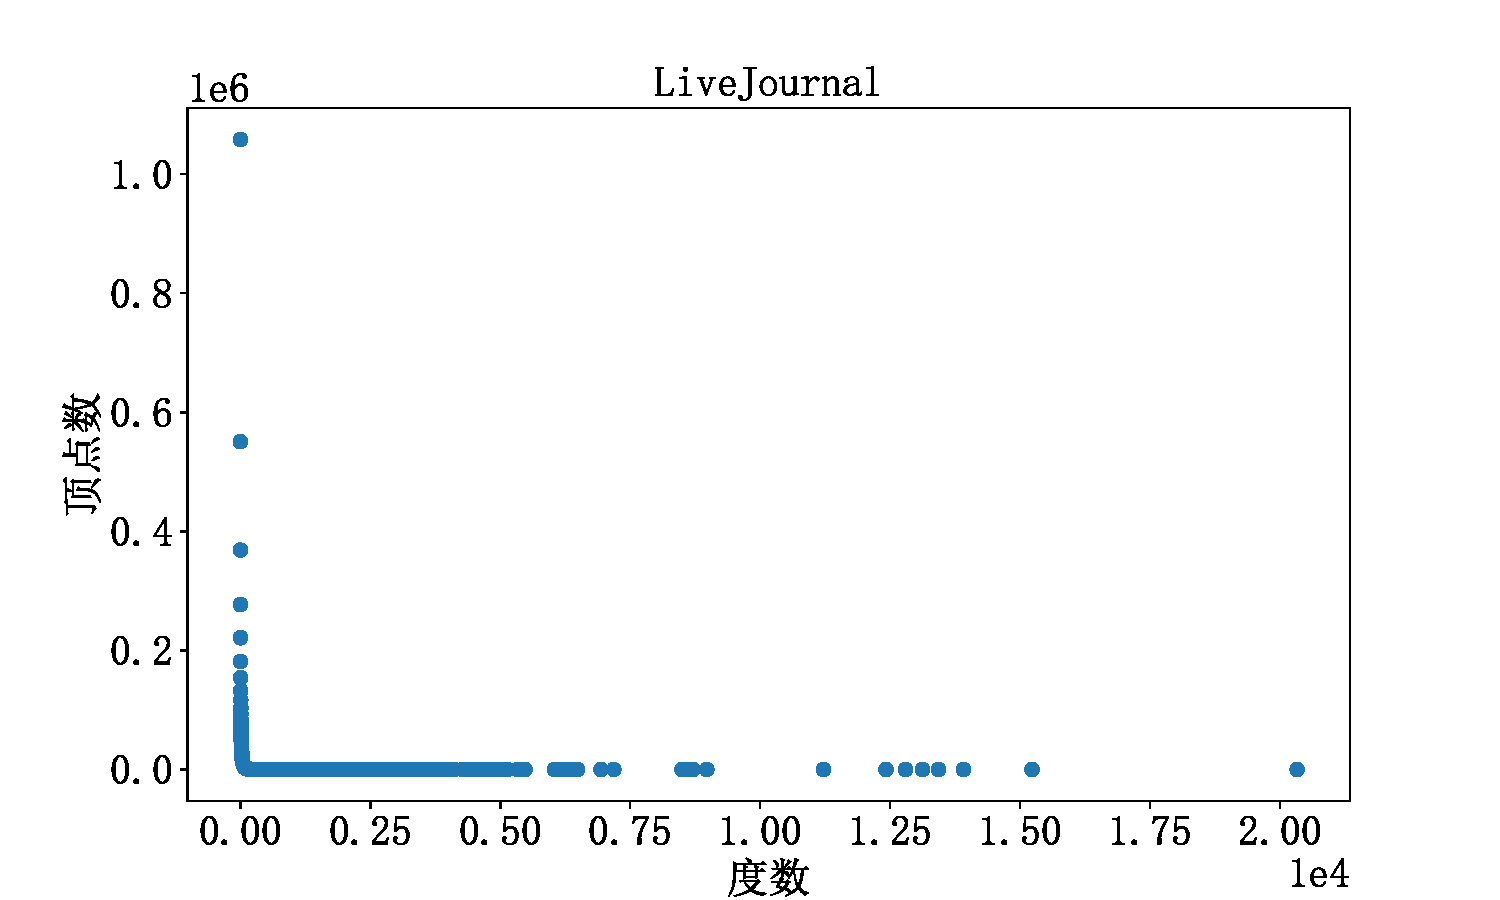
\includegraphics[width=0.5\linewidth]{pic/vertex/LiveJournal.pdf}%
    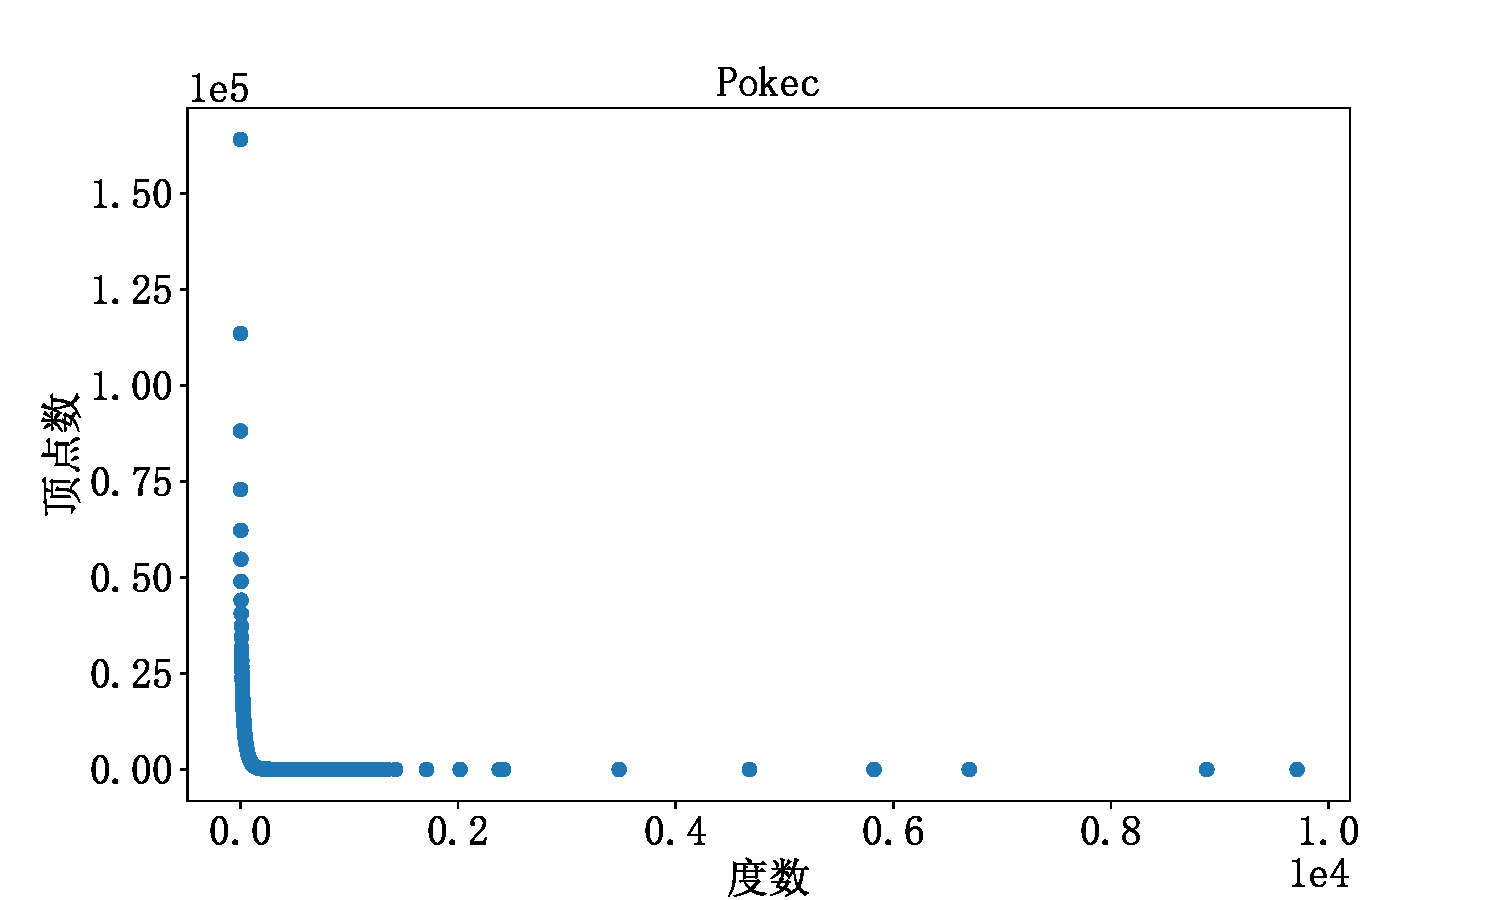
\includegraphics[width=0.5\linewidth]{pic/vertex/Pokec.pdf}\\
    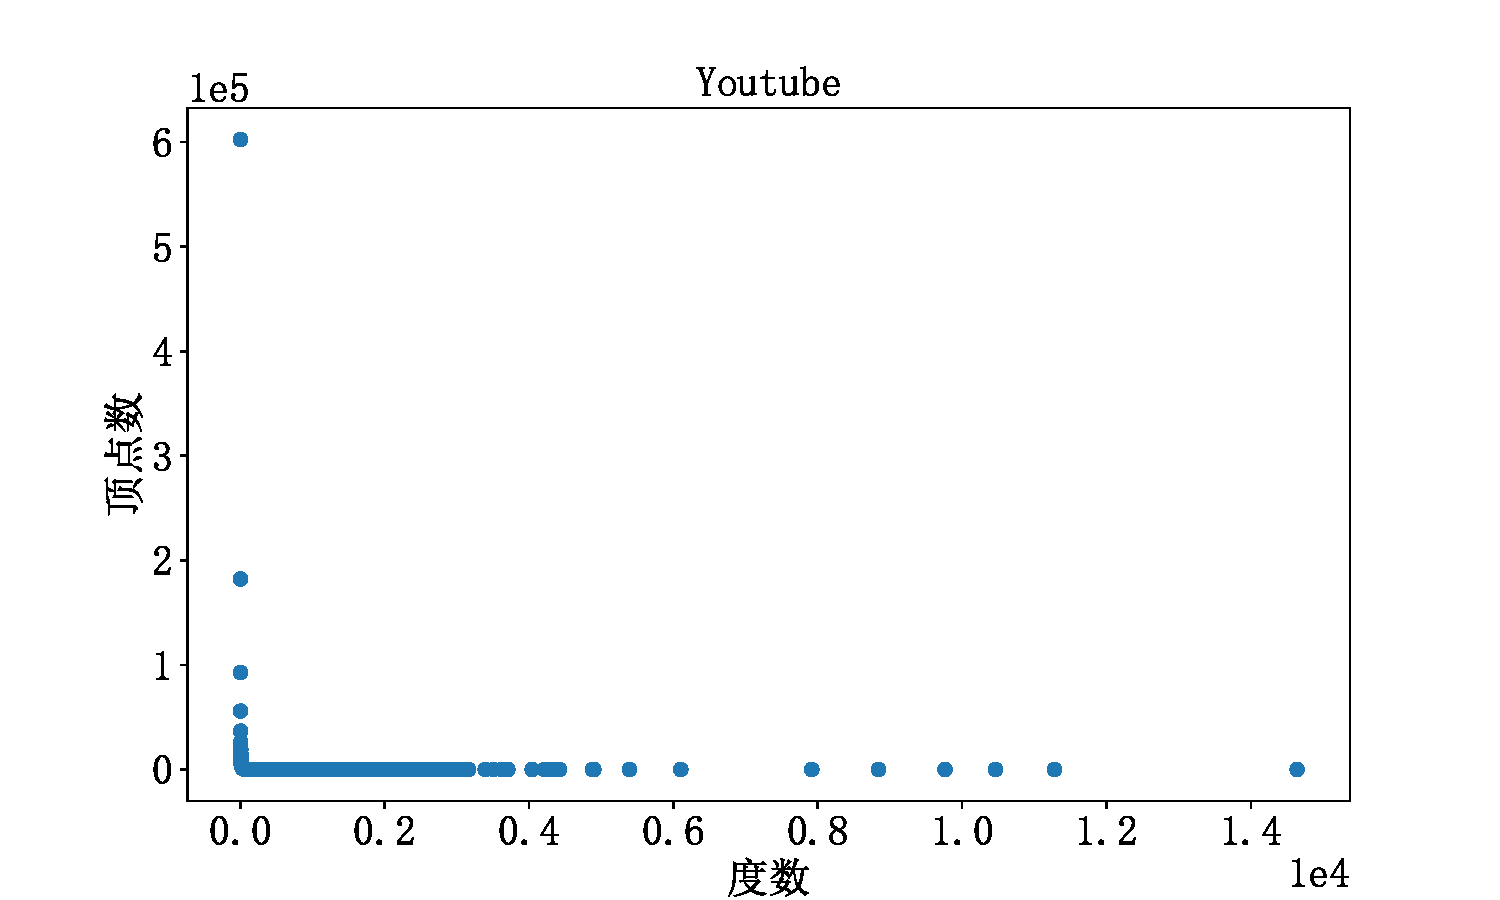
\includegraphics[width=0.5\linewidth]{pic/vertex/Youtube.pdf}%
    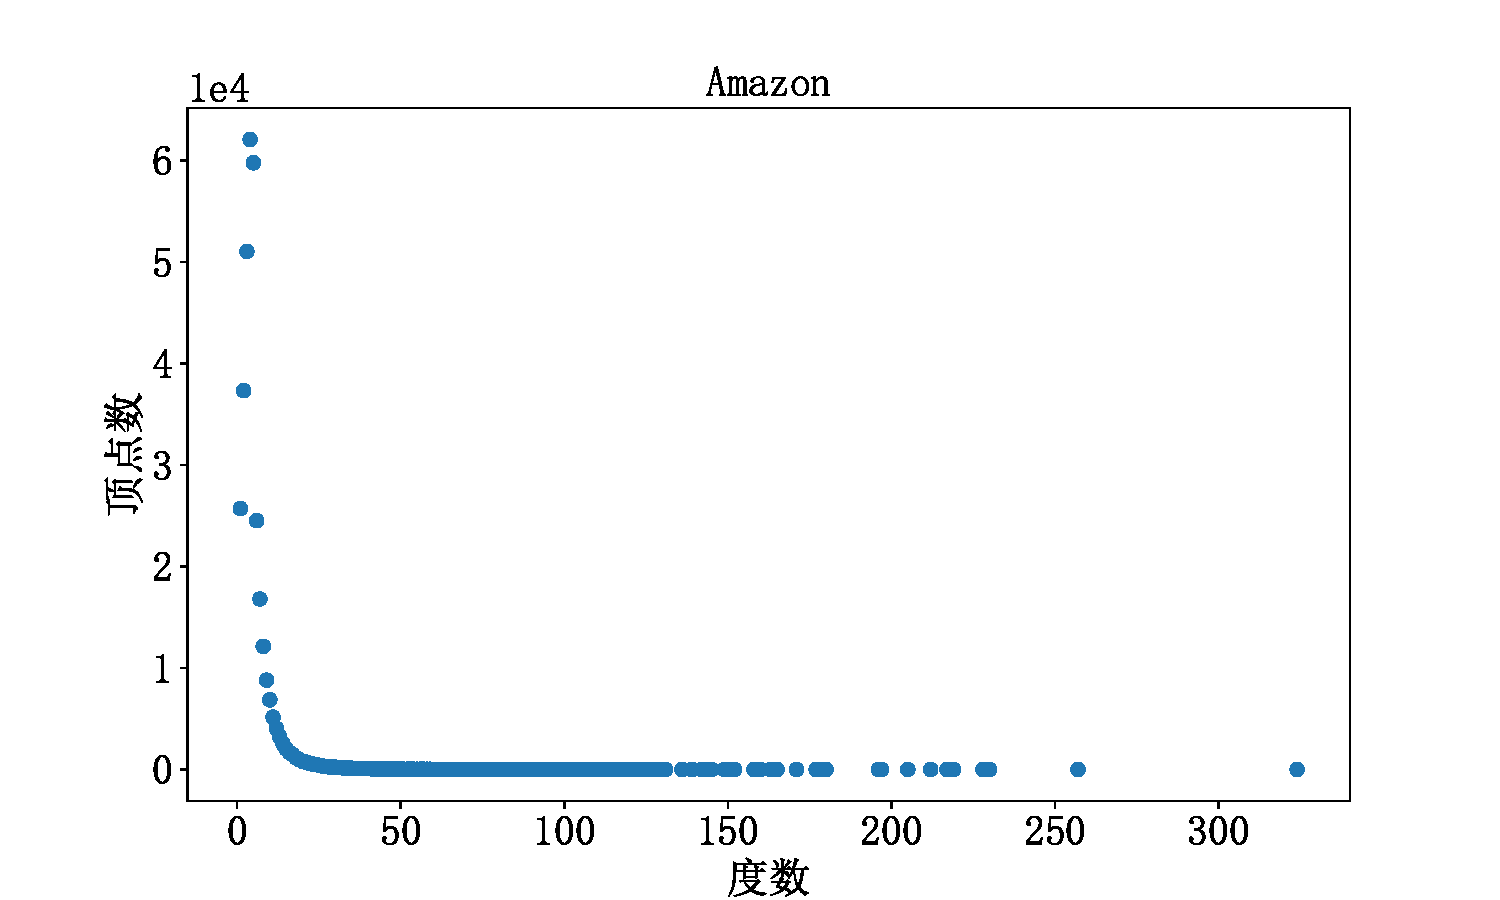
\includegraphics[width=0.5\linewidth]{pic/vertex/Amazon.pdf}\\
    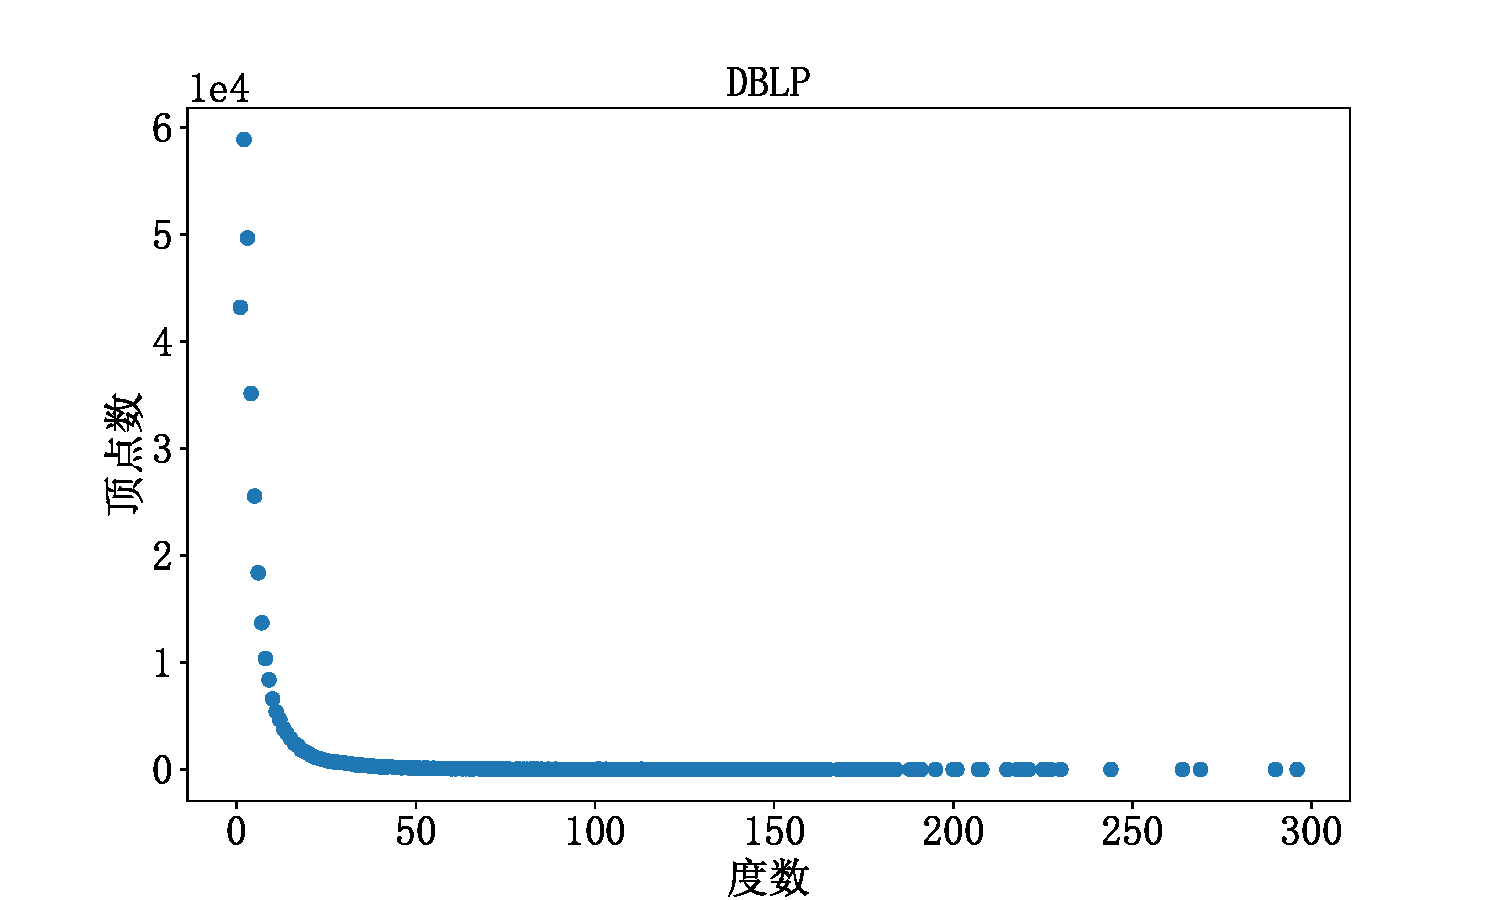
\includegraphics[width=0.5\linewidth]{pic/vertex/DBLP.pdf}%
    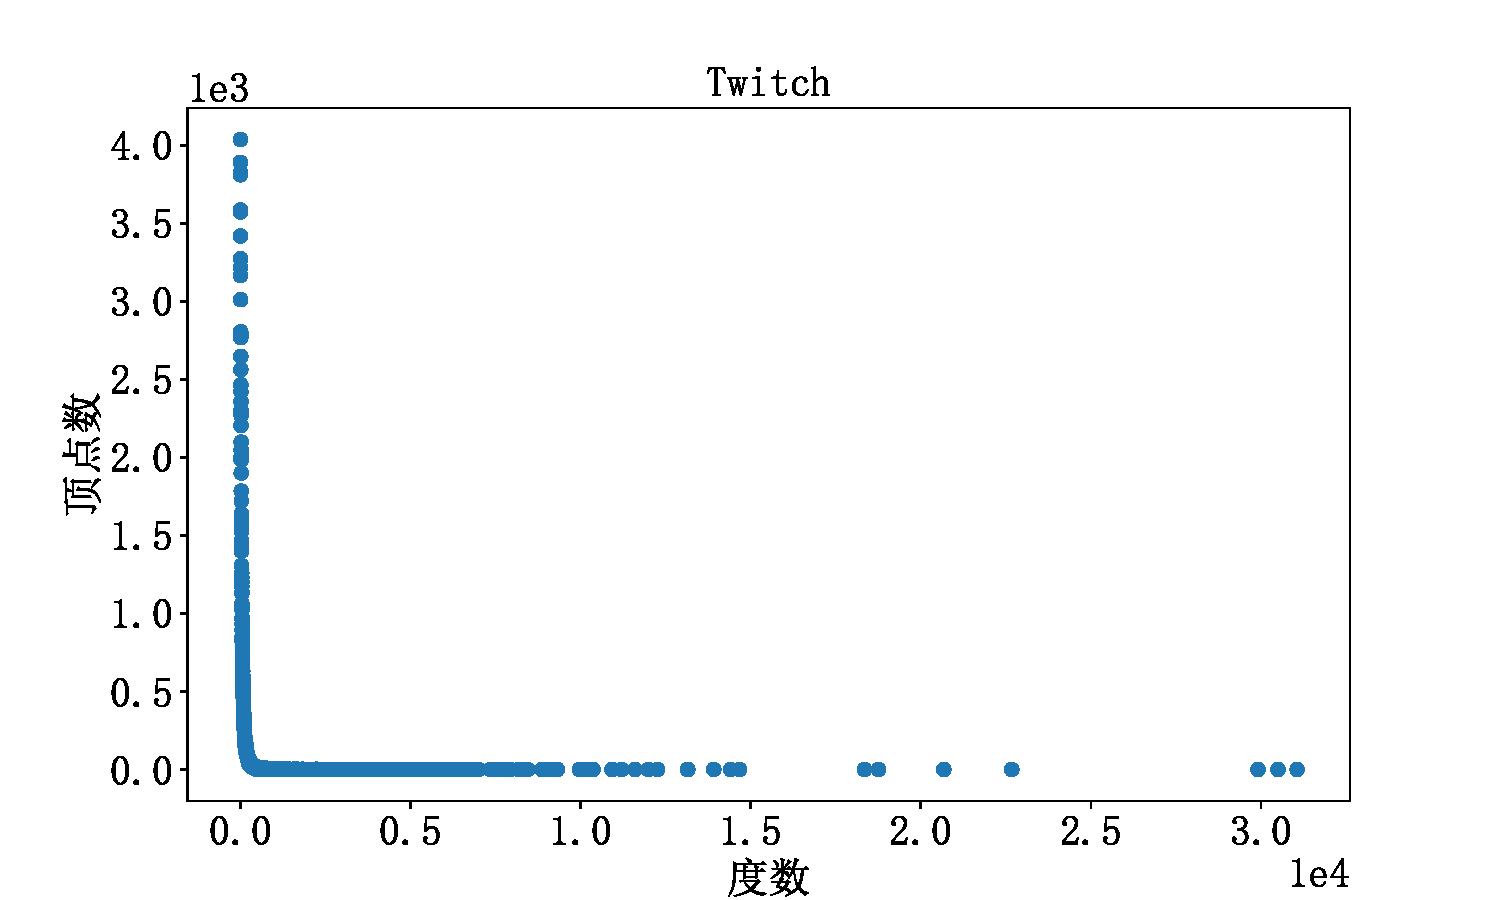
\includegraphics[width=0.5\linewidth]{pic/vertex/Twitch.pdf}\\
    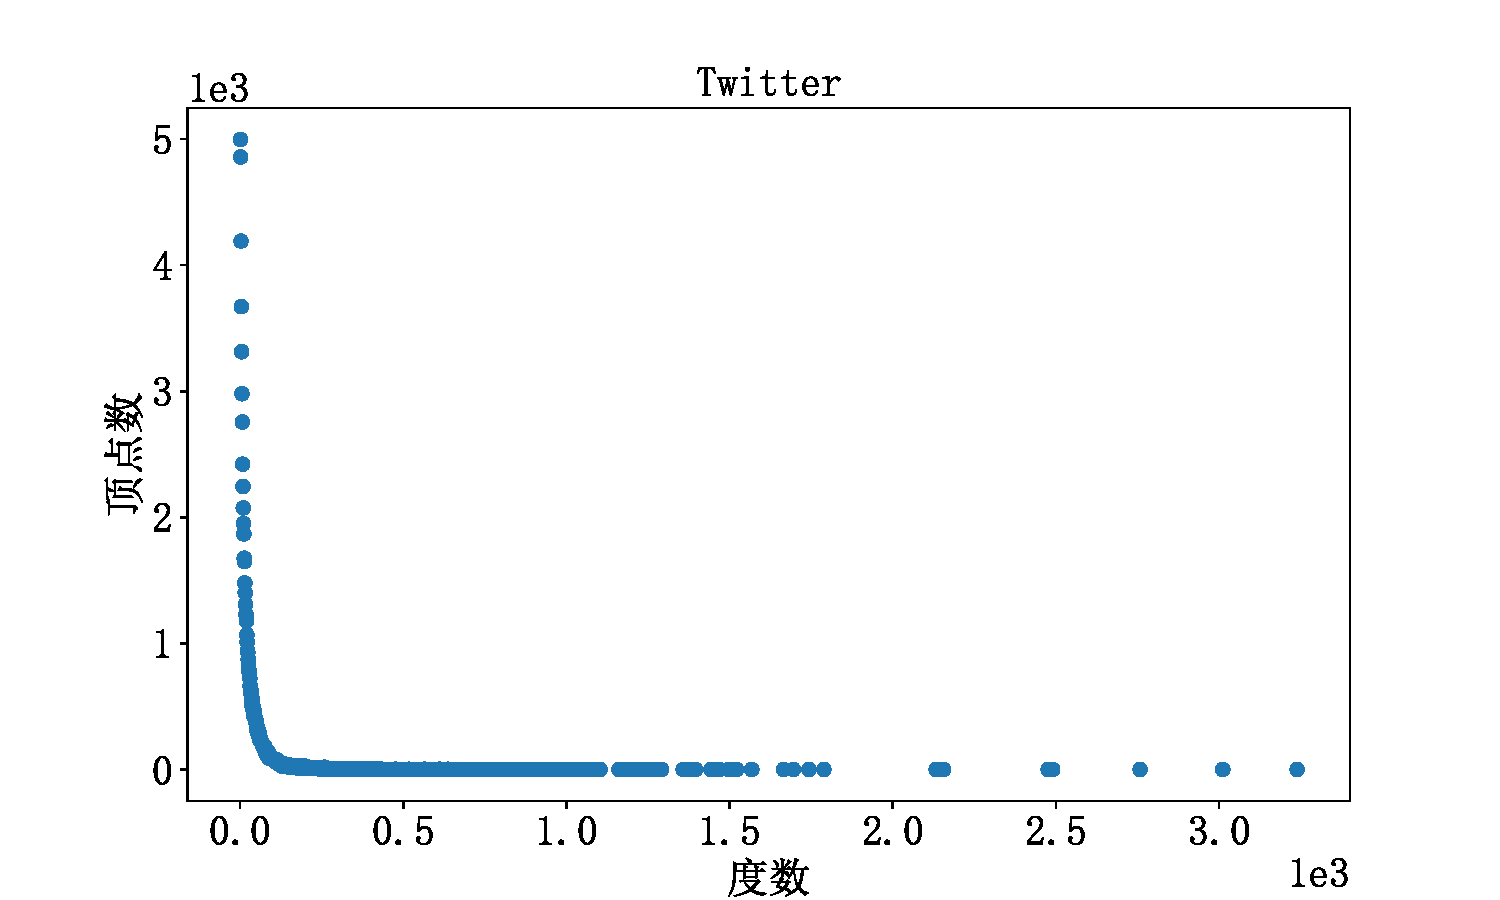
\includegraphics[width=0.5\linewidth]{pic/vertex/Twitter.pdf}%
    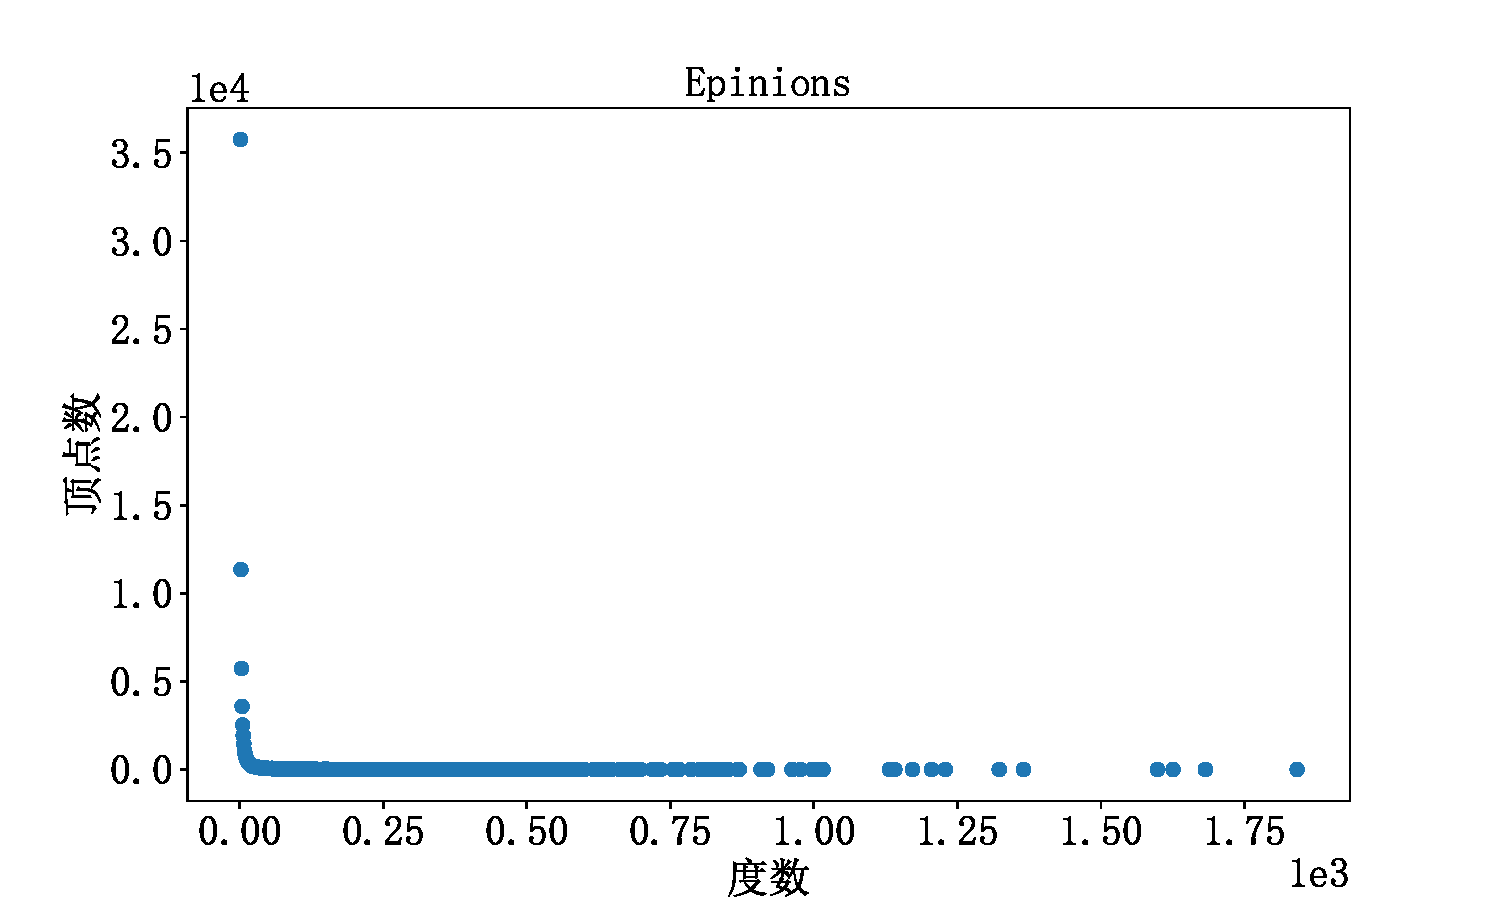
\includegraphics[width=0.5\linewidth]{pic/vertex/Epinions.pdf}\\
    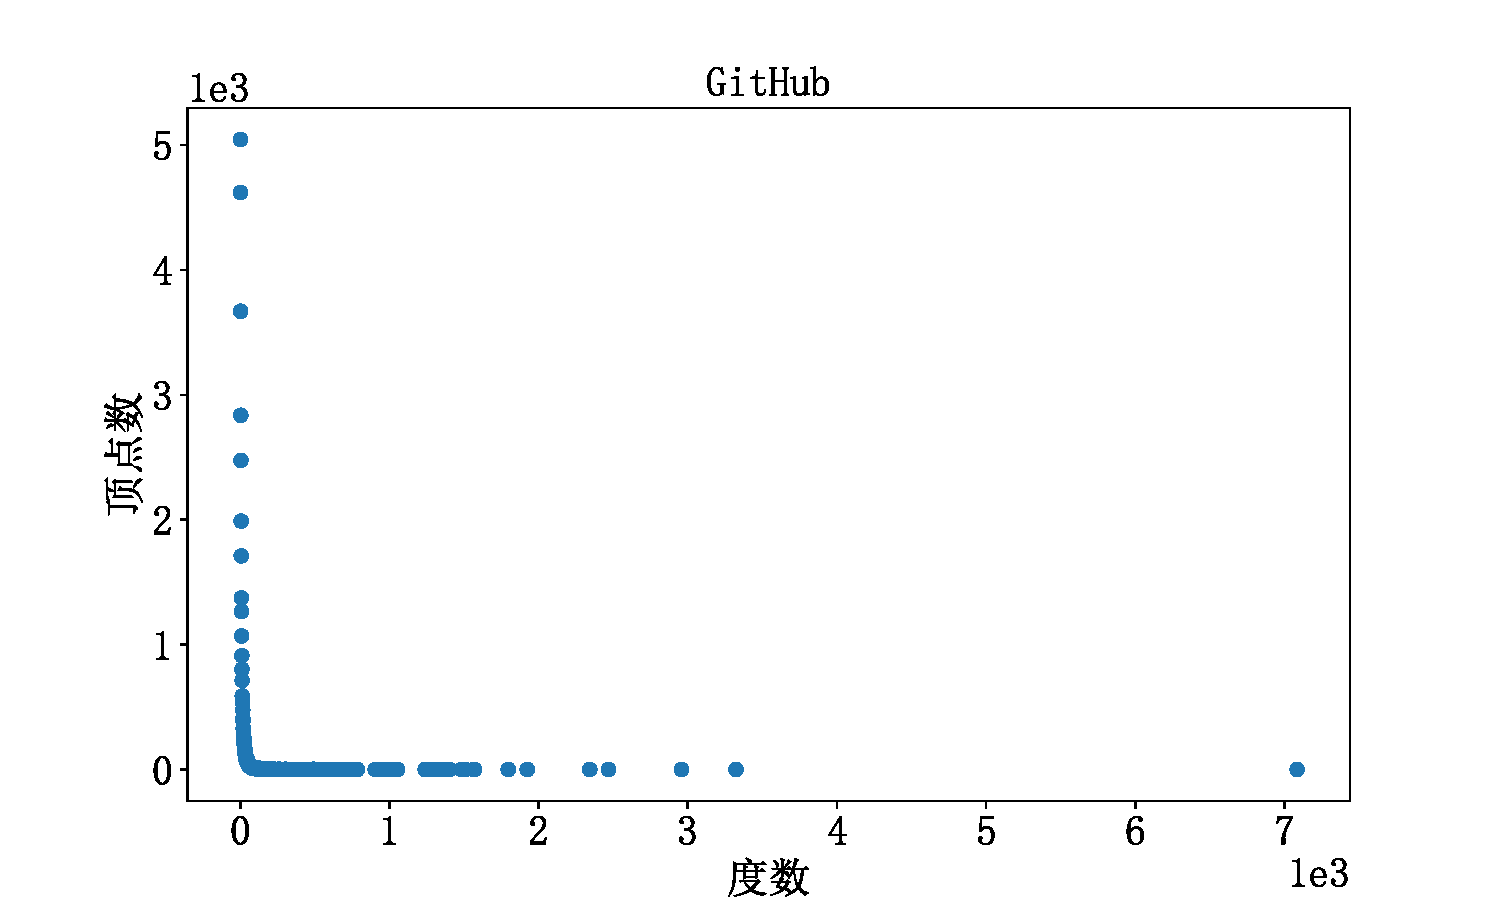
\includegraphics[width=0.5\linewidth]{pic/vertex/GitHub.pdf}%
    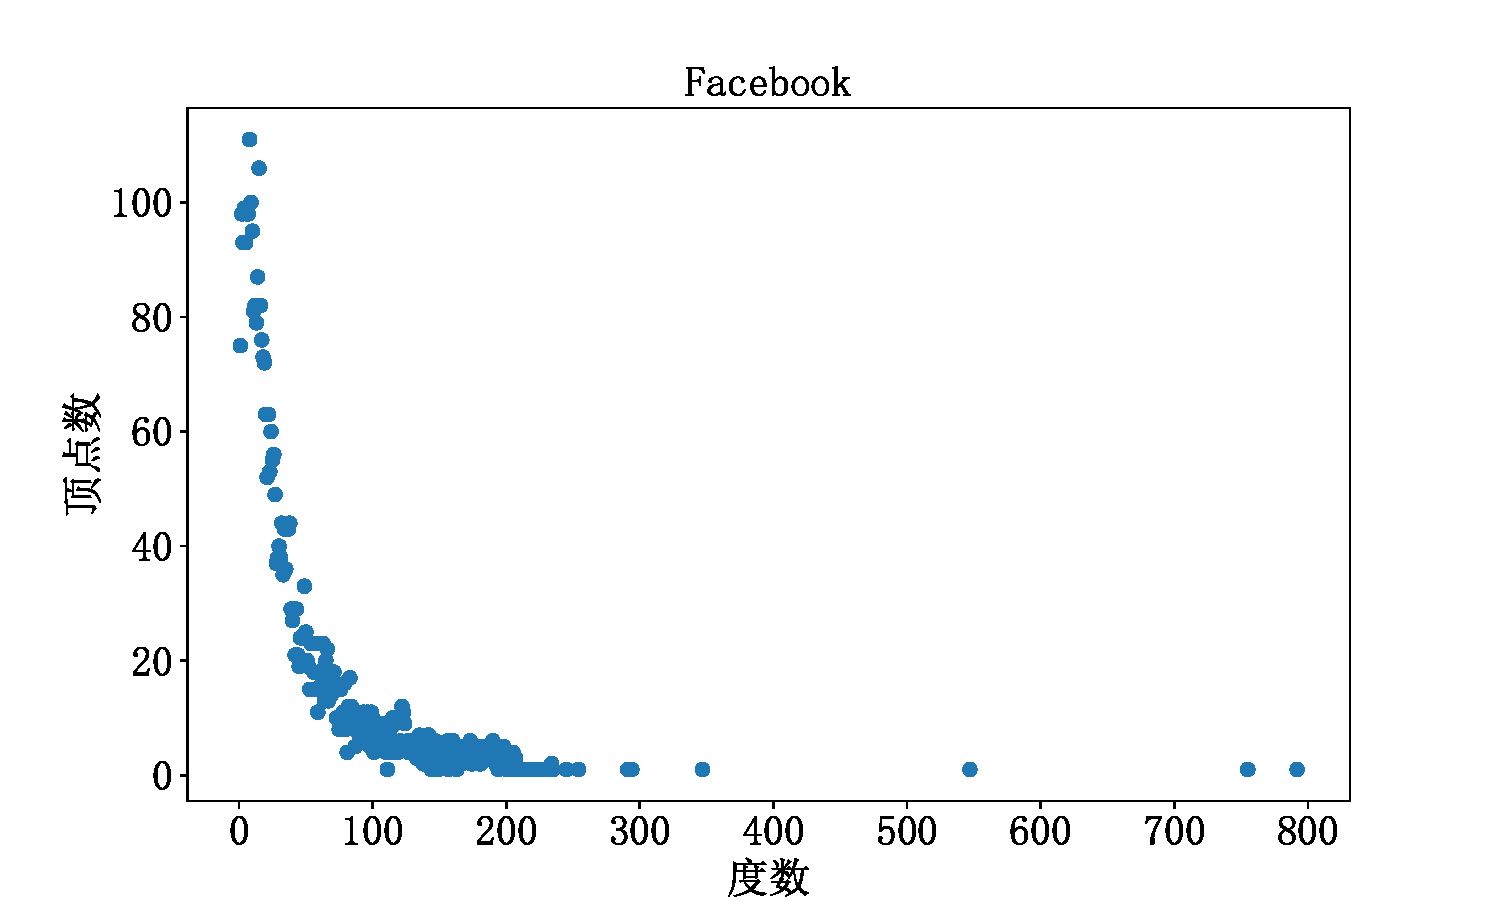
\includegraphics[width=0.5\linewidth]{pic/vertex/Facebook.pdf}
    \caption{度数与顶点的幂律关系}
    \label{fig:pow-law-vertex}
\end{figure}
    幂律分布在真实世界图数据集中广泛存在,它表示不同度数$d$与该度数的顶点数$v(d)$之间的关系,即$v(d)=C·d^{-k}$。
在图\ref{fig:pow-law-vertex}中显示了不同数据集的度数与顶点分布,显然都满足幂律关系。
然后可以推导出特定度数和该度数顶点的连接边数$e(d)$之间的映射关系,如式\ref{eq:edge-deg}所示,该式也遵循幂律。
\begin{equation}
    e(d)=v(d) \cdot d=C \cdot d^{-k} \cdot d=C \cdot d^{-k+1}
    \label{eq:edge-deg}
\end{equation}
    
    通常情况下,顶点的度数越大,边数越多,构成模式的概率越大。一个直观的猜测是度数与模式数量分布也呈现幂律
关系(度数对应的模式数定义为该度数顶点所形成的模式数量)。因此,假设特定度数的模式$p(d)$满足:
\begin{equation}
    p(d)=C_0 \cdot d^{-\alpha}+C_1, \quad\left(C_0>0, C_1>0\right)
    \label{eq:pattern-deg}
\end{equation}

    对于模式计数问题,需要的最终结果是整个图数据集中模式的总出现次数,本文通过式子\ref{eq:pattern-deg-cumu}中
的累积分布函数$P(d)$来计算。
\begin{equation}
    \label{eq:pattern-deg-cumu}
    \begin{split}
    P(d) & \approx \int_1^d{p(x)}\mathrm{d}x = \frac{C_0}{-\alpha+1}d^{-\alpha+1} + C_2 \\
        & = Ad^{-\beta} + B \quad (A < 0, B > 0, \beta > 0)
    \end{split}
\end{equation}

    本文选择三角形计数在多个具有代表性图数据集上进行了测试。测试获得了数据集边数和模式数的分布情况如图\ref{fig:pattern-edge-dis}。

   
\begin{figure}
    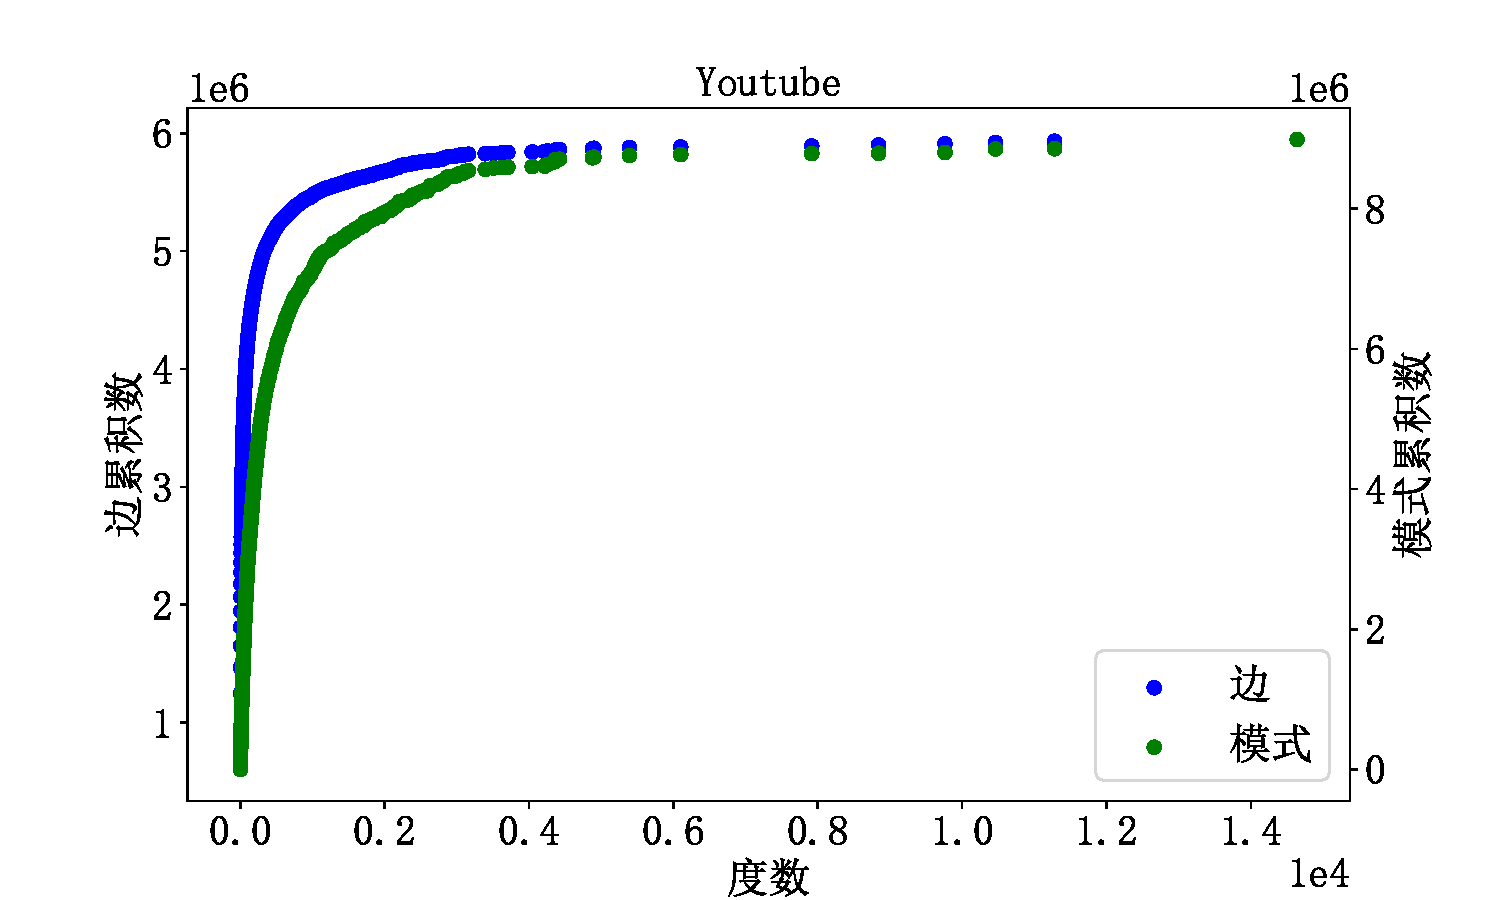
\includegraphics[width=0.5\linewidth]{pic/powerlaw/Youtube.pdf}%
    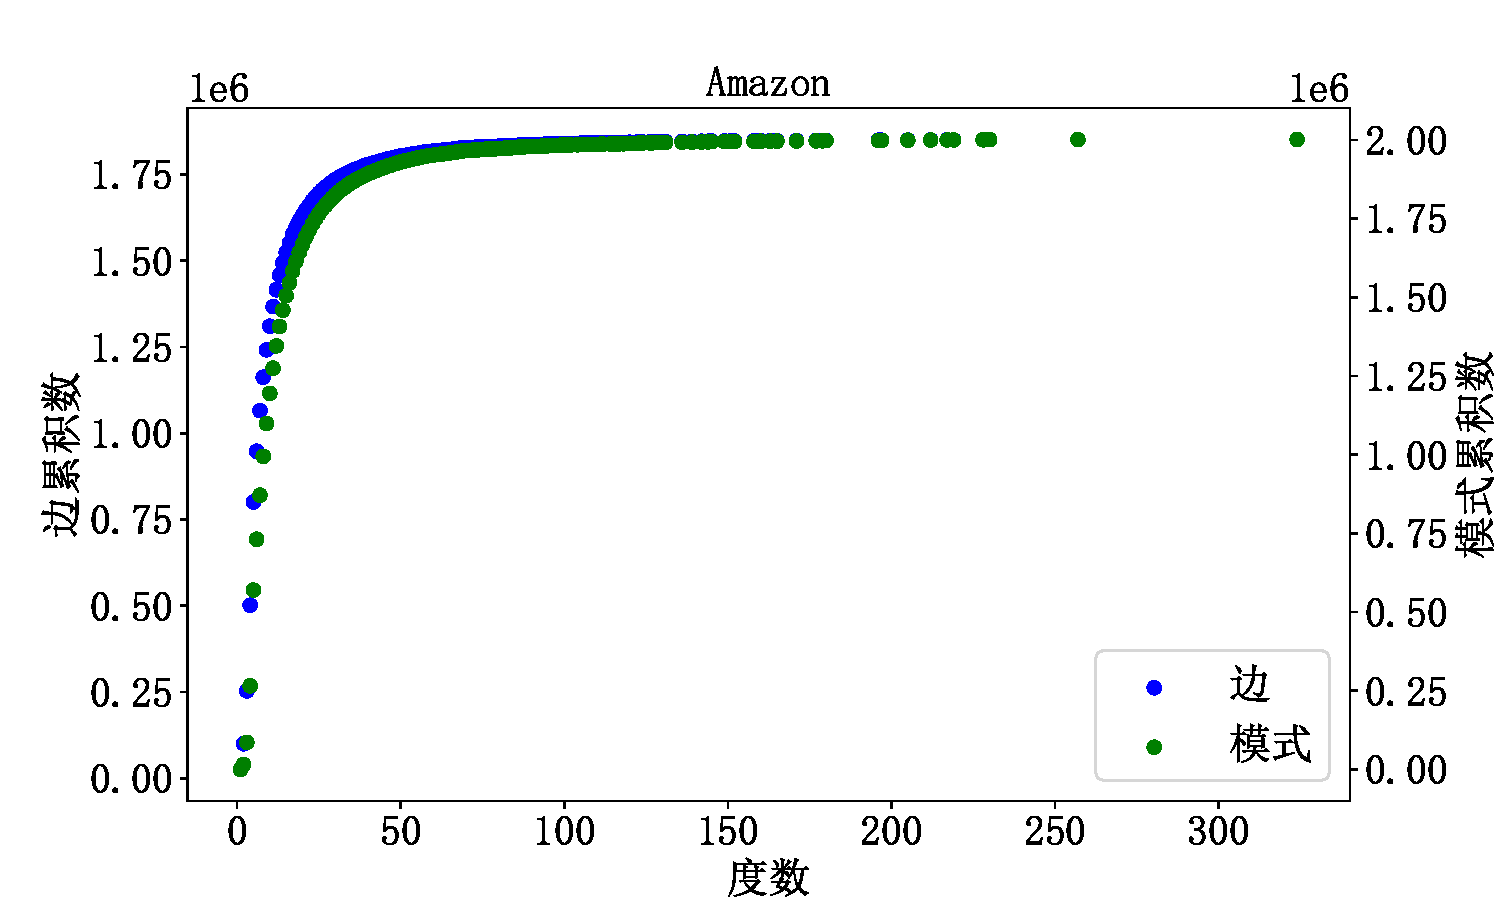
\includegraphics[width=0.5\linewidth]{pic/powerlaw/Amazon.pdf}\\
    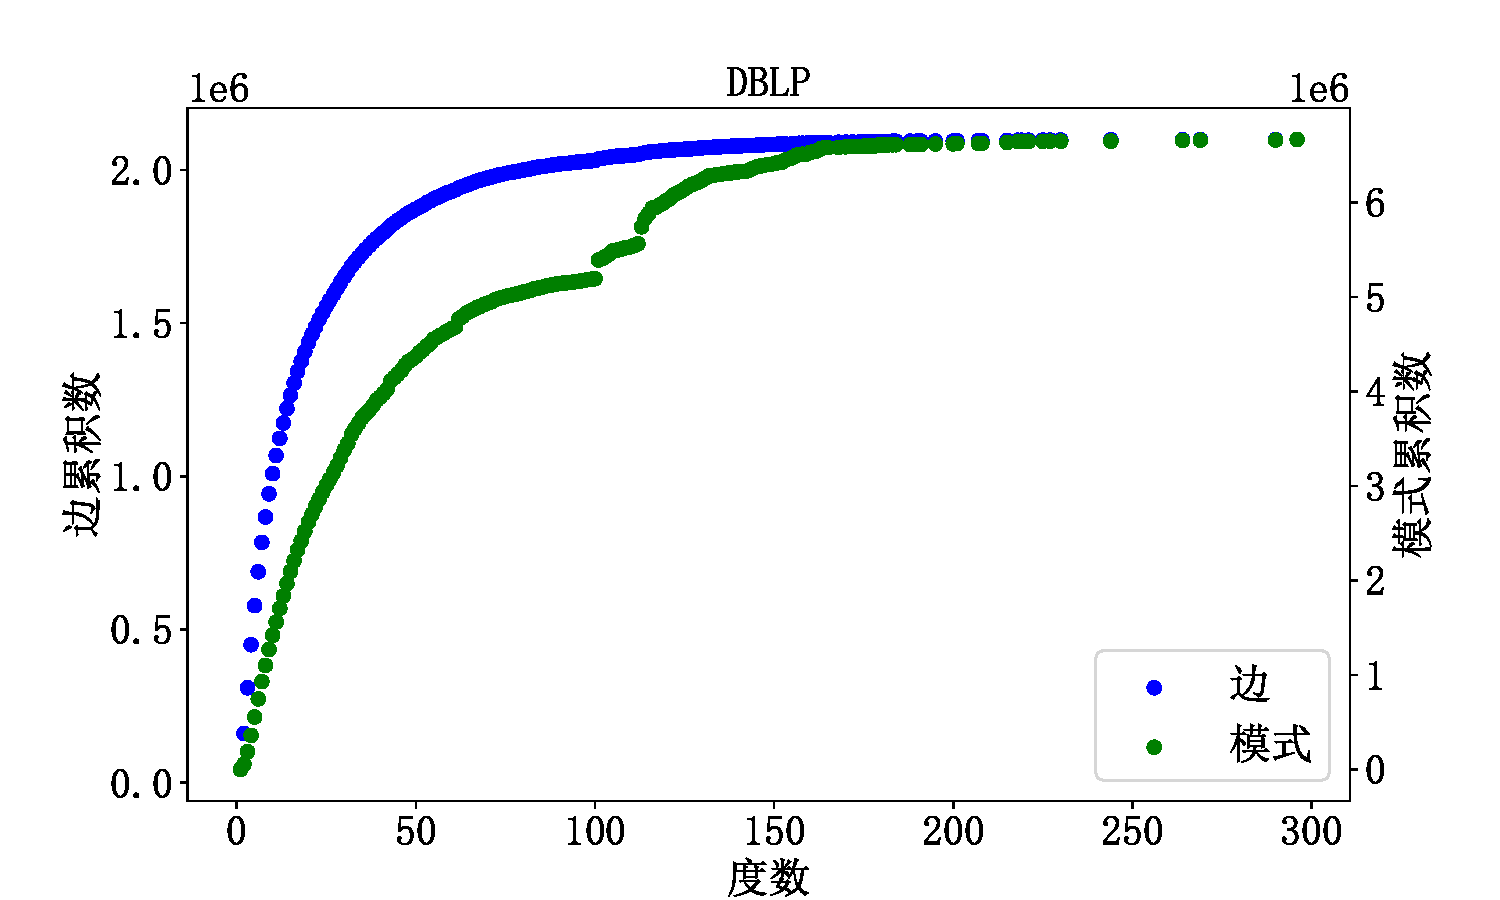
\includegraphics[width=0.5\linewidth]{pic/powerlaw/DBLP.pdf}%
    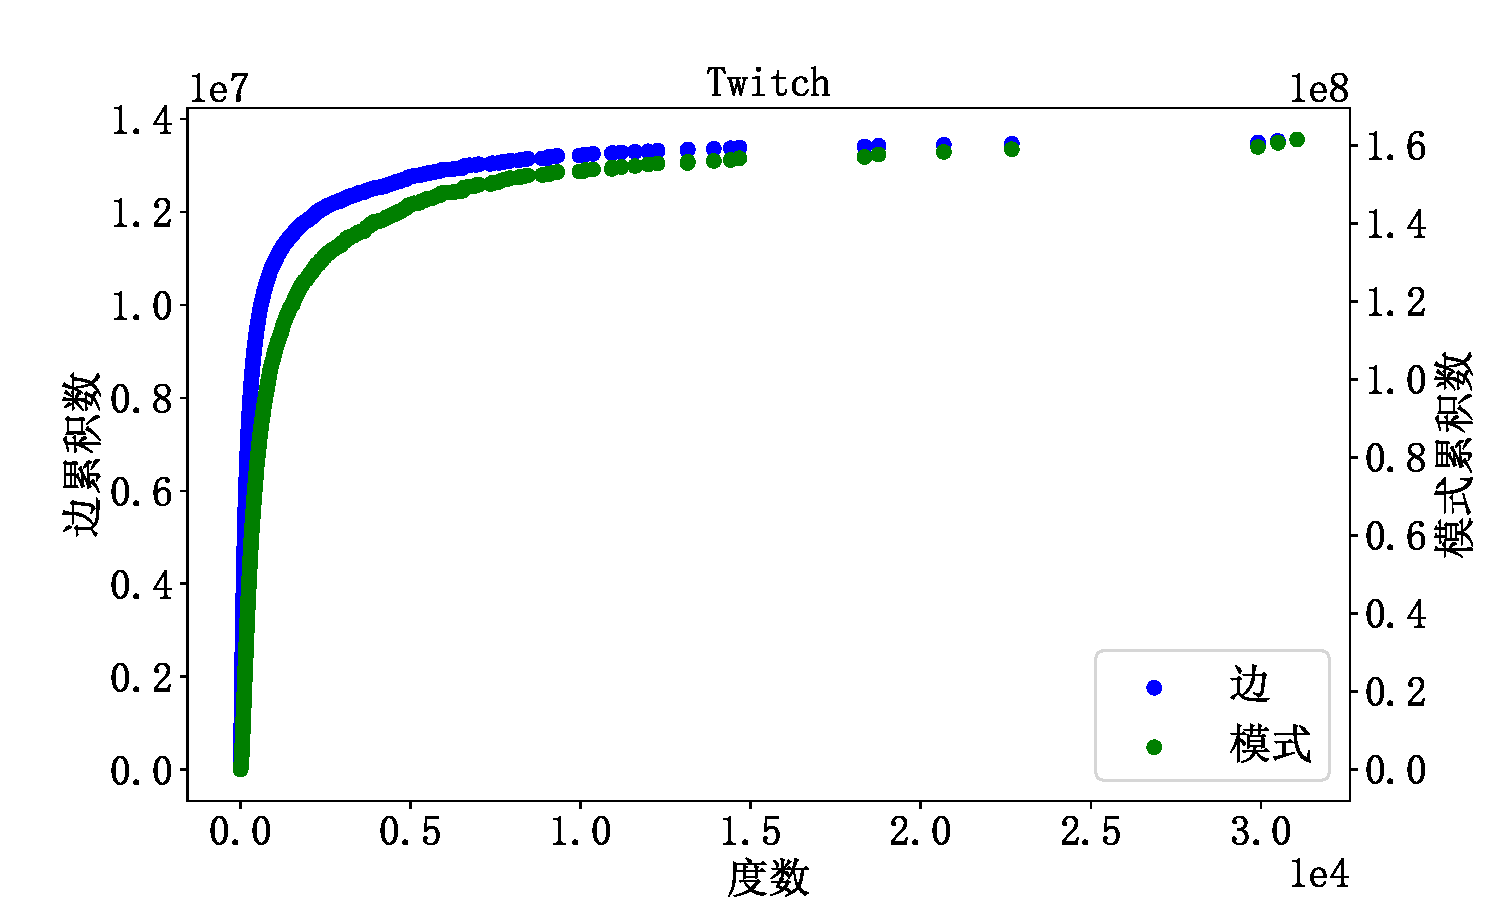
\includegraphics[width=0.5\linewidth]{pic/powerlaw/Twitch.pdf}\\
    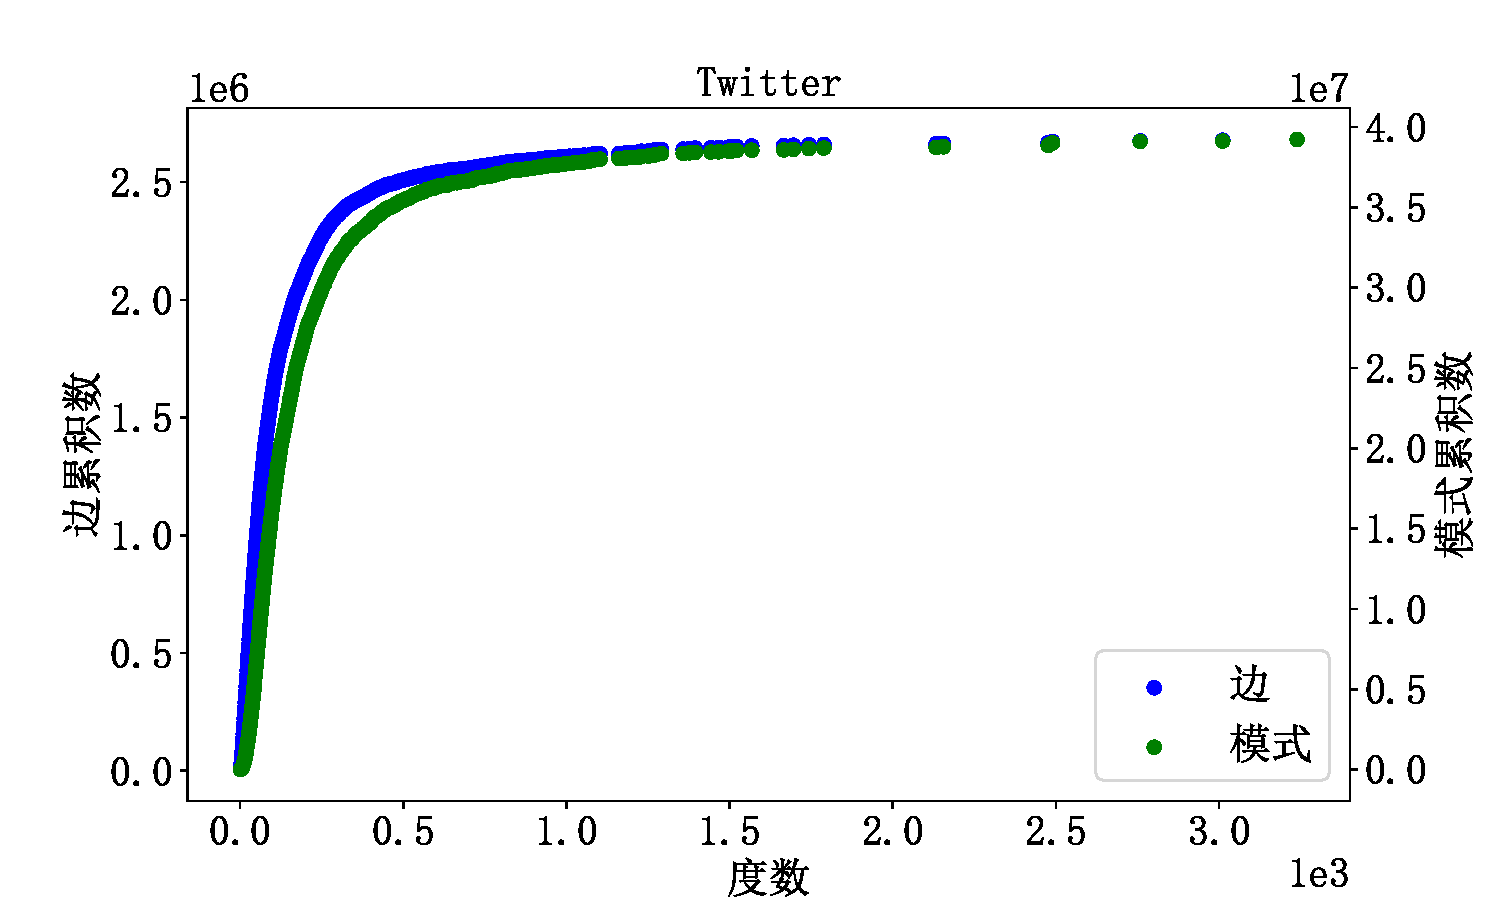
\includegraphics[width=0.5\linewidth]{pic/powerlaw/Twitter.pdf}%
    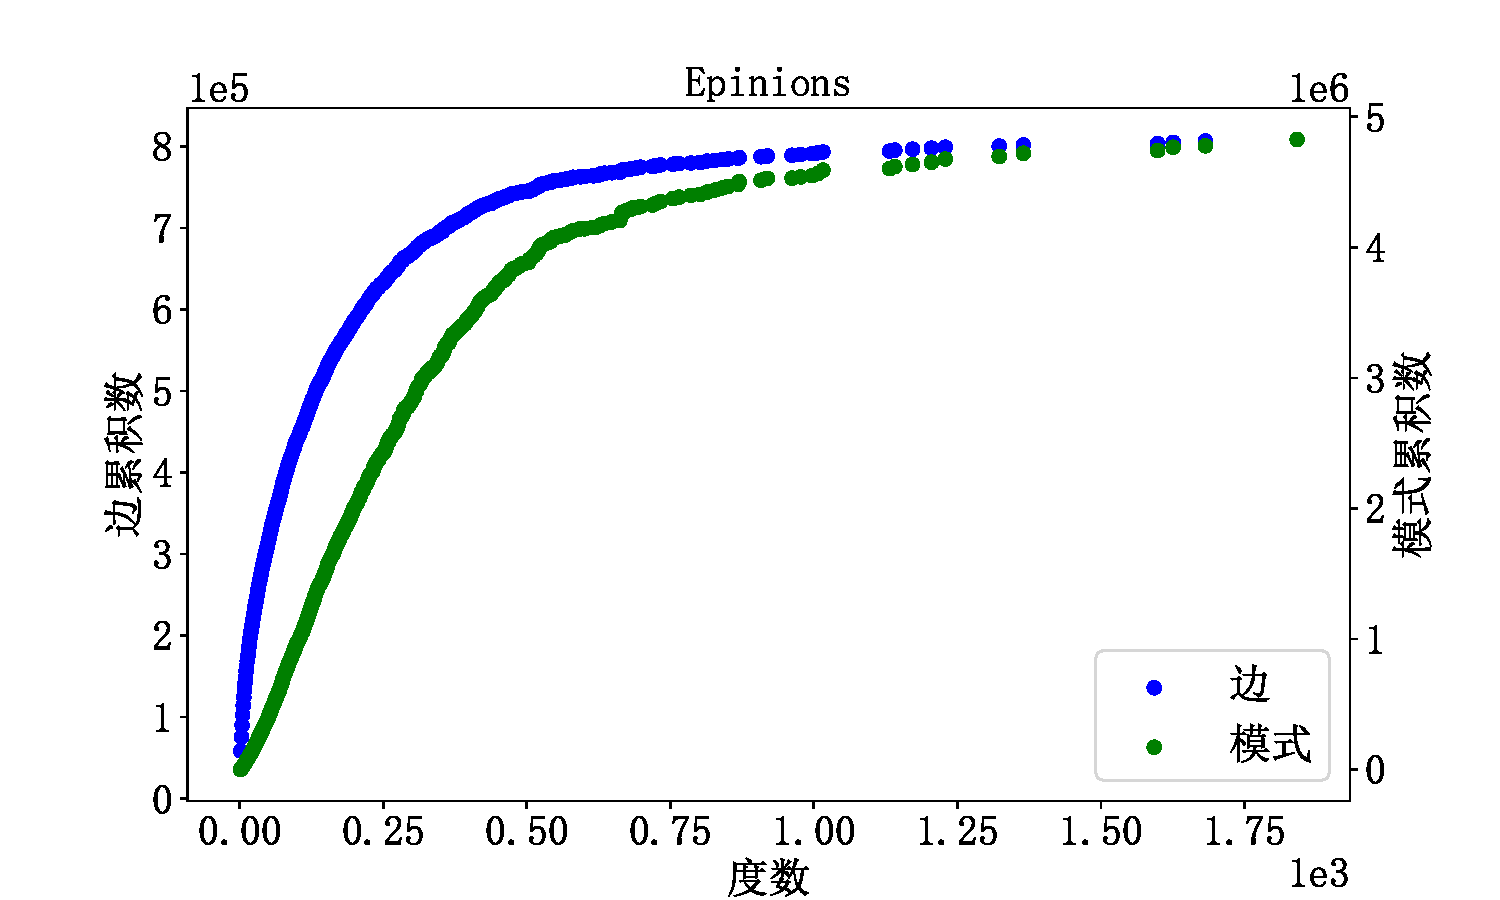
\includegraphics[width=0.5\linewidth]{pic/powerlaw/Epinions.pdf}\\
    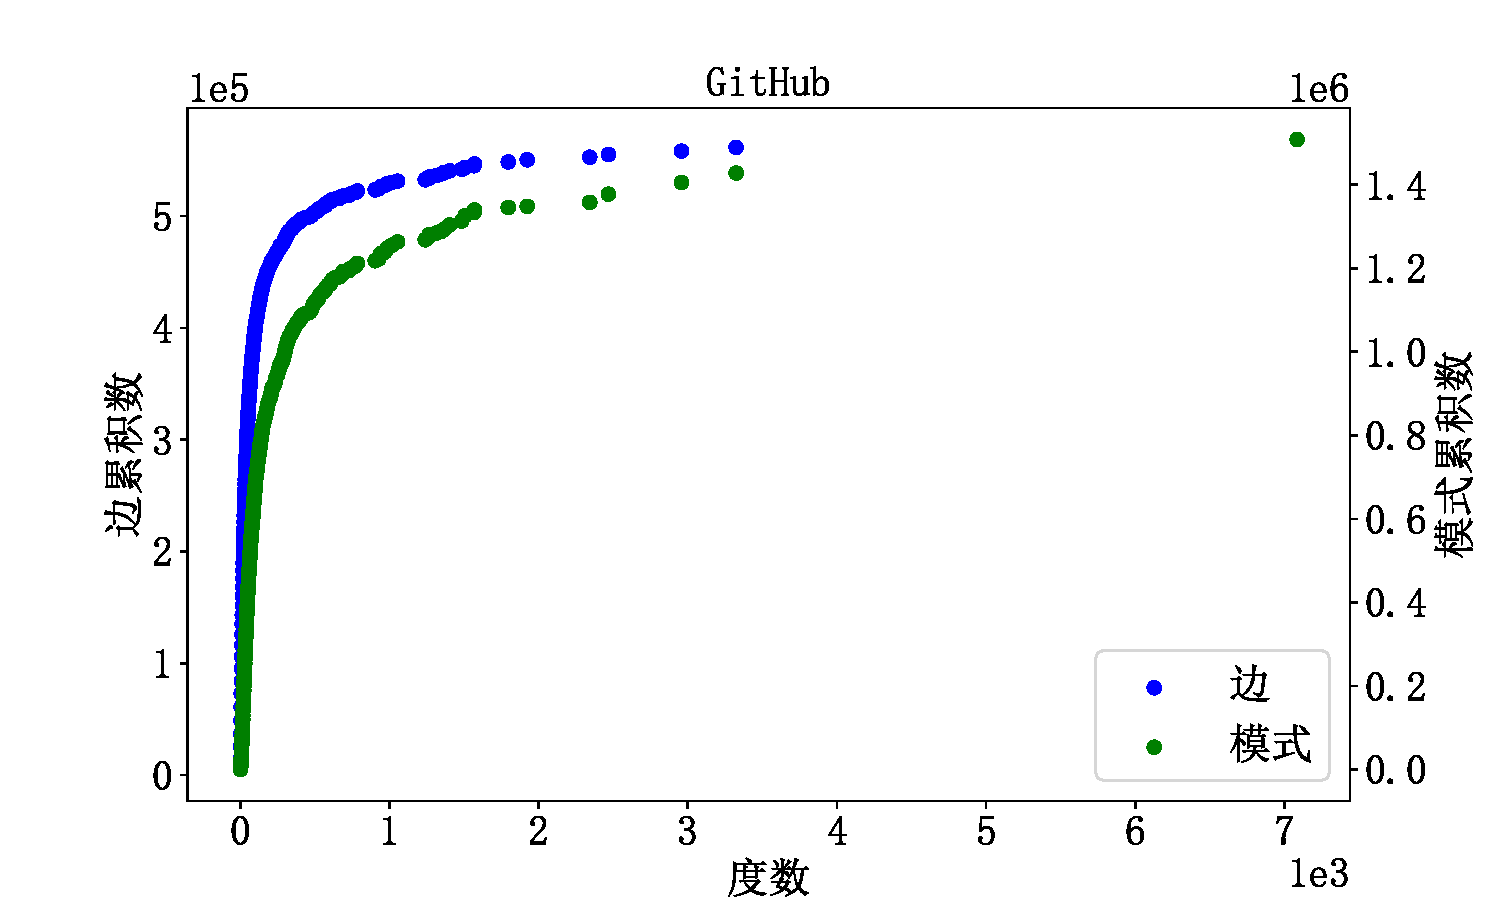
\includegraphics[width=0.5\linewidth]{pic/powerlaw/GitHub.pdf}%
    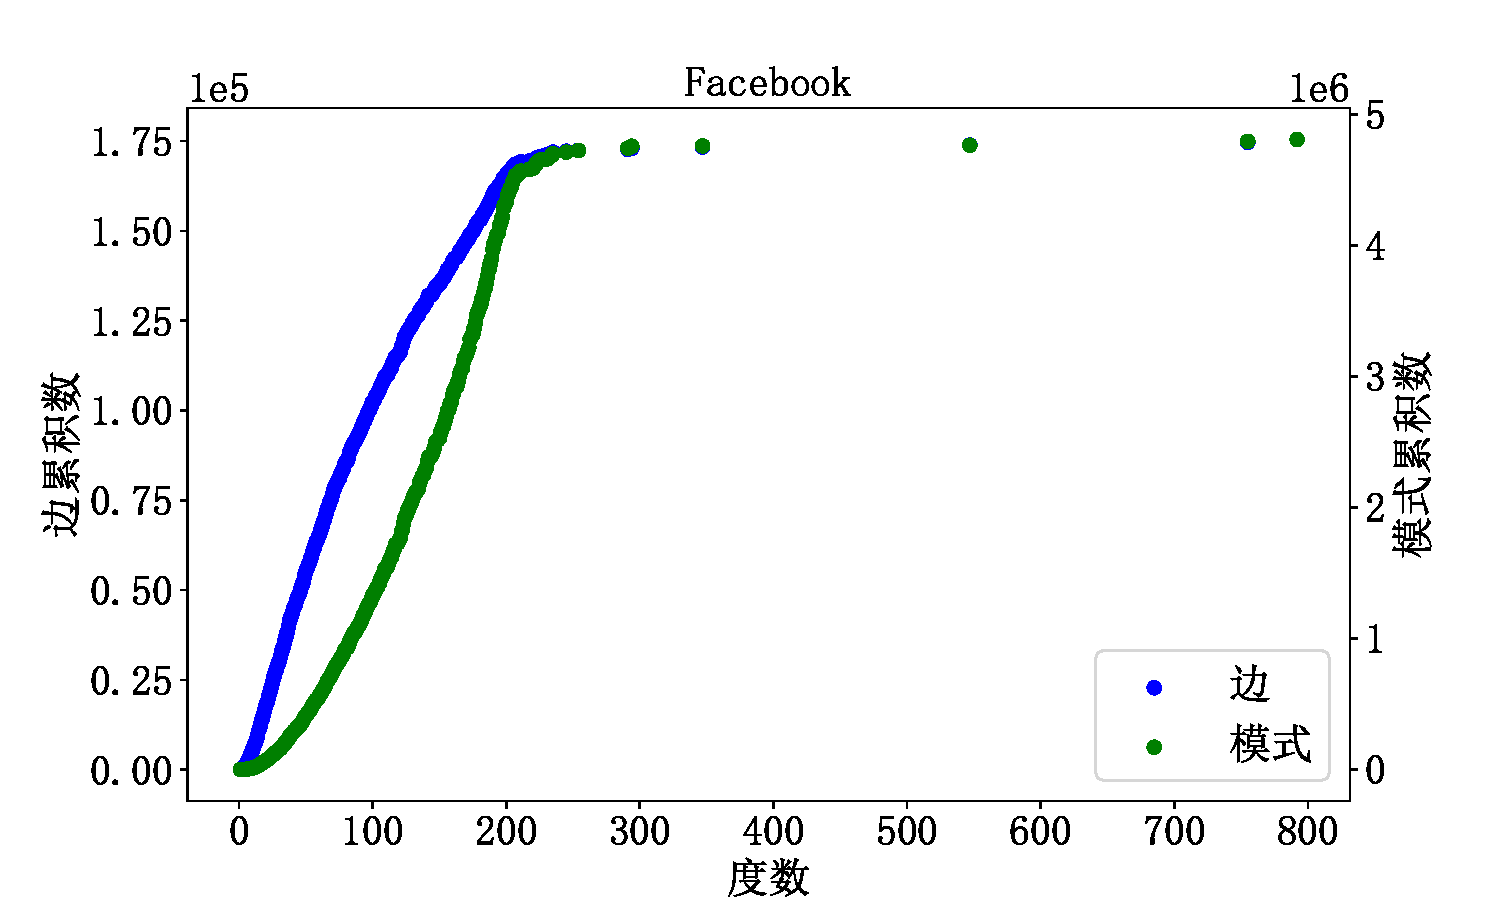
\includegraphics[width=0.5\linewidth]{pic/powerlaw/Facebook.pdf}
    \caption{模式累积分布与边累积分布}
    \label{fig:pattern-edge-dis}
\end{figure}

    图\ref{fig:pattern-edge-dis}展示了不同数据集的边累积分布与模式累积分布。边累积分布表示了小于等于当前度数(横轴值)
的所有边数之和(纵轴值),模式累积分布同理。基于对分布情况,本文提出以下观点:
\begin{itemize}
    
    \item 在多个数据集中,边-度数累积分布普遍比模式-度数累积分布更"凸",这表示高度数顶点的连接边构成模式的概率更大:
    边累积和占总边数50\%时,对应度数的模式累积和不足50\%,则说明剩余50\%的边提供了更多的模式数。
    因此可以基于传统的邻域采样方法,将采样的重心偏向高度数边,以此增加模式被采样的概率,提高估计精度。
    
    \item 图数据集的模式累积分布都显示幂律分布特征,式\ref{eq:pattern-deg-cumu}具有普遍性。
    因此可以通过收集模式累积分布曲线中少量的数据点,使用非线性回归对式\ref{eq:pattern-deg-cumu}进行拟合,来估算模式总数。
    由于不用在数据集的全部边集数组中进行扫描,可以进一步降低执行时间,同时保证足够的精度。
\end{itemize}

    基于以上观察,本文系统整体设计如下。

\section{整体架构设计}
\label{sec:overall-architecture}
    本文针对图数据集的图数据幂律分布特性,设计系统整体架构,目的是提高图模式近似挖掘的执行速度,减少估计误差。
首先在近似算法执行前对图数据进行预处理,对图的边集存储顺序进行调整,并生成帮助采样过程的数据结构。
接着本文使用两种思路进行图模式近似挖掘:基于幂律属性的模式采样估计方法,使用区间划分策略和估计器选择策略来优化图
近似模式挖掘中的传统领域采样算法;基于幂律属性的模式分布模型构建技术,对模式的幂律分布模型进行非线性回归
拟合曲线来计算来计算结果,这是一种新的估计方法。
 
\begin{figure}
    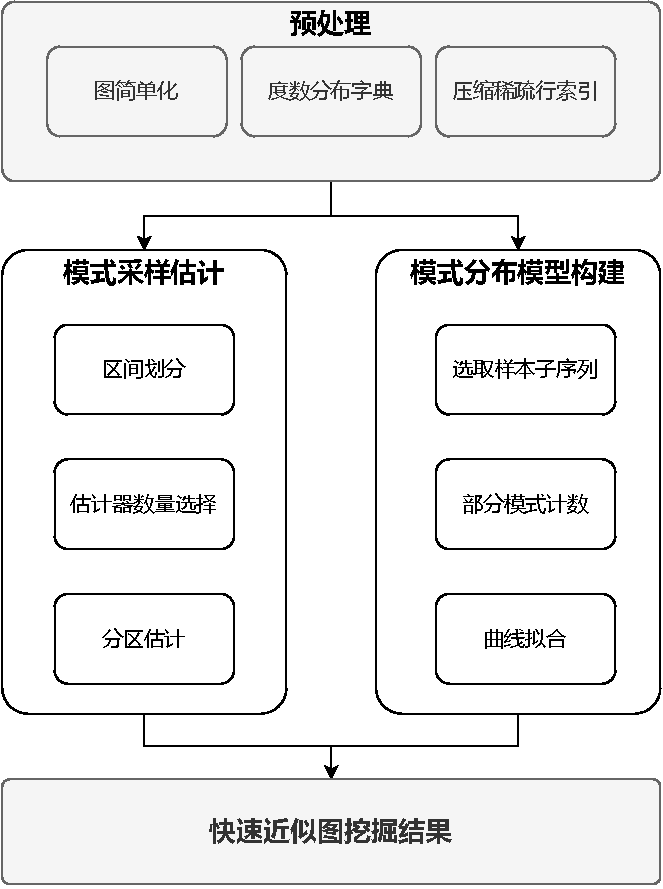
\includegraphics{overall_architecture.pdf}
	\caption{整体架构}
	\label{fig:over_architecture}
\end{figure}
    
    在图\ref{fig:over_architecture}中展示了整体架构的三个模块:预处理模块、模式采样估计模块、模式分布模型构建模块。
\section{预处理模块设计}
\label{sec:preprocessing-module}
    预处理是对大规模数据进行处理的常见手段,作用是调整数据集、收集数据集基本属性,便于后续处理。本文设计预处理模块在
近似算法开始之前,先对图数据集进行处理。预处理模块根据度数信息调整图的边集存储顺序,生成能够加速算法执行的数据结构,
为后续步骤中模式采样估计模块和模式分布模型构建模块提供帮助。

\subsection{图简单化}
\label{subsec:simplification}

    本文在模式采样估计模块中以邻域采样算法作为基础进行优化,在模式分布模型构建模块中也使用邻域采样算法你作为获取
模式计数的方法之一,包含平行边和自环的非简单图将导致邻域采样算法错误。因此还需要对图数据集进行简单化,
去除平行边和自环。

    在无向图中,关联一对顶点的无向边如果多于1条,则称这些边为平行边,平行边的条数称为重数。在有向图中,关联一对顶
点的有向边如果多于1条,并且这些边的始点与终点相同(也就是它们的的方向相同),称这些边为平行边。如果一条边的两端连接
同一个顶点,则称这条边为自环。根据图论,既不含平行边也不包含自环的图称为简单图。

\begin{figure}
    \subfloat[自环]{
        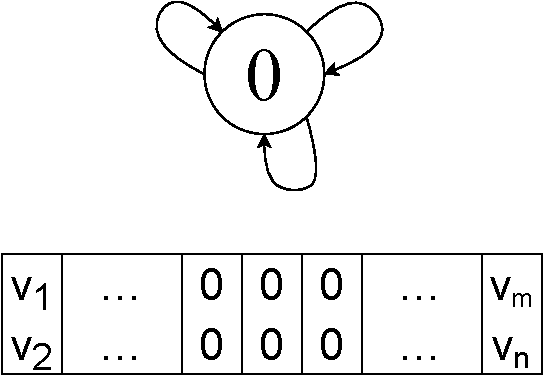
\includegraphics[width=.3\linewidth]{pic/simp_selfloop.pdf}
        \label{pic:simp-selfloop}
    }
    \subfloat[平行边]{
        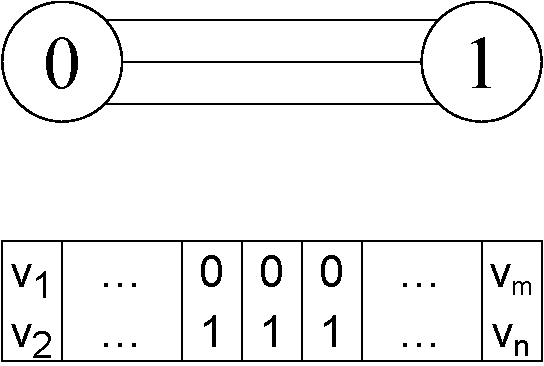
\includegraphics[width=.3\linewidth]{pic/simp_multiedge.pdf}
        \label{pic:simp-multiedge}
    }
    \subfloat[平行边和自环]{
        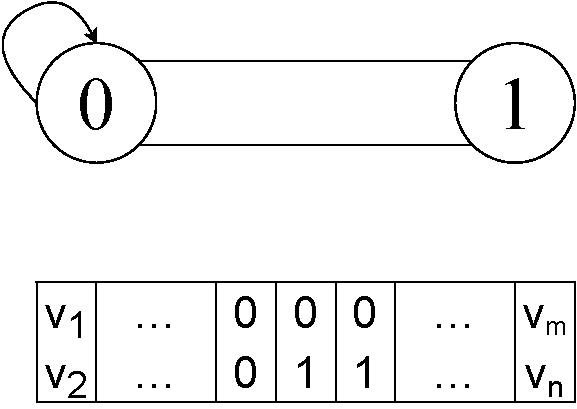
\includegraphics[width=.3\linewidth]{pic/simp_selfloop_multiedges.pdf}
        \label{pic:simp-selfloop-multiedge}
    }
    \caption{平行边和自环导致邻域采样中三角形计数错误示例}
    \label{pic:simp-error}
\end{figure}

    在模式挖掘中,如果不对平行边和自环进行处理,邻域采样算法都会产生错误,图\ref{pic:simp-error}描述了这种错误。图
\ref{pic:simp-selfloop}中包含三条两端顶点为$(0,0)$的自环,其中每个自环的邻域都会包含其他两个自环。假如
图\ref{subsec:neighbor}中的邻域采样算法采样到的前两条边都是$(0,0)$,算法将会在后续边集中寻找$(0,0)$,因而将
三条自环边错误的计数为三角形。同理,在\ref{pic:simp-multiedge}中有三条平行边$(0,1)$,在\ref{pic:simp-selfloop-multiedge}
中自环和平行边同时出现,也会导致类似的错误。


\subsection{度数重排序}
\label{subsec:reorder}
    
    由于图数据集的边集数组通常是随机顺序排列的,如果模式采样估计模块直接在边集数组中进行采样,将会均等对待不同度数的边,
没有优先考虑高度数边对模式的贡献,导致效率不高。因此预处理模块对图数据集进行度数重排序,增加高度数边被采样的概率。

    边集数组中边按照顶点对$(SrcID,DstID)$的形式存储,$SrcID$表示源顶点的唯一标识,$DstID$表示目标顶点的唯一标识。
有向图中$(SrcID,DstID)$表述方向为$SrcId$指向$DstID$,无向图中不表示方向。对边集数组进行遍历,获取每个顶点的度数。然后
按照度数升序对顶点进行排序,度数相同则按原本顶点ID排序。赋予排序后的顶点新的ID,在后文\ref{subsec:csr}中将要描述压缩
稀疏行索引,其中位置数组根据顶点ID直接寻址,因此新ID从0开始编号。根据新ID和旧ID对应关系,将边集数组中的边进行
$(SrcID,DstID)$升序排列,即首先按$SrcID$升序排列,如果$SrcID$相同则按$DstID$升序排列。排序后的边集数组能够保证源顶点
度数相同边相邻排列。
\begin{figure}
    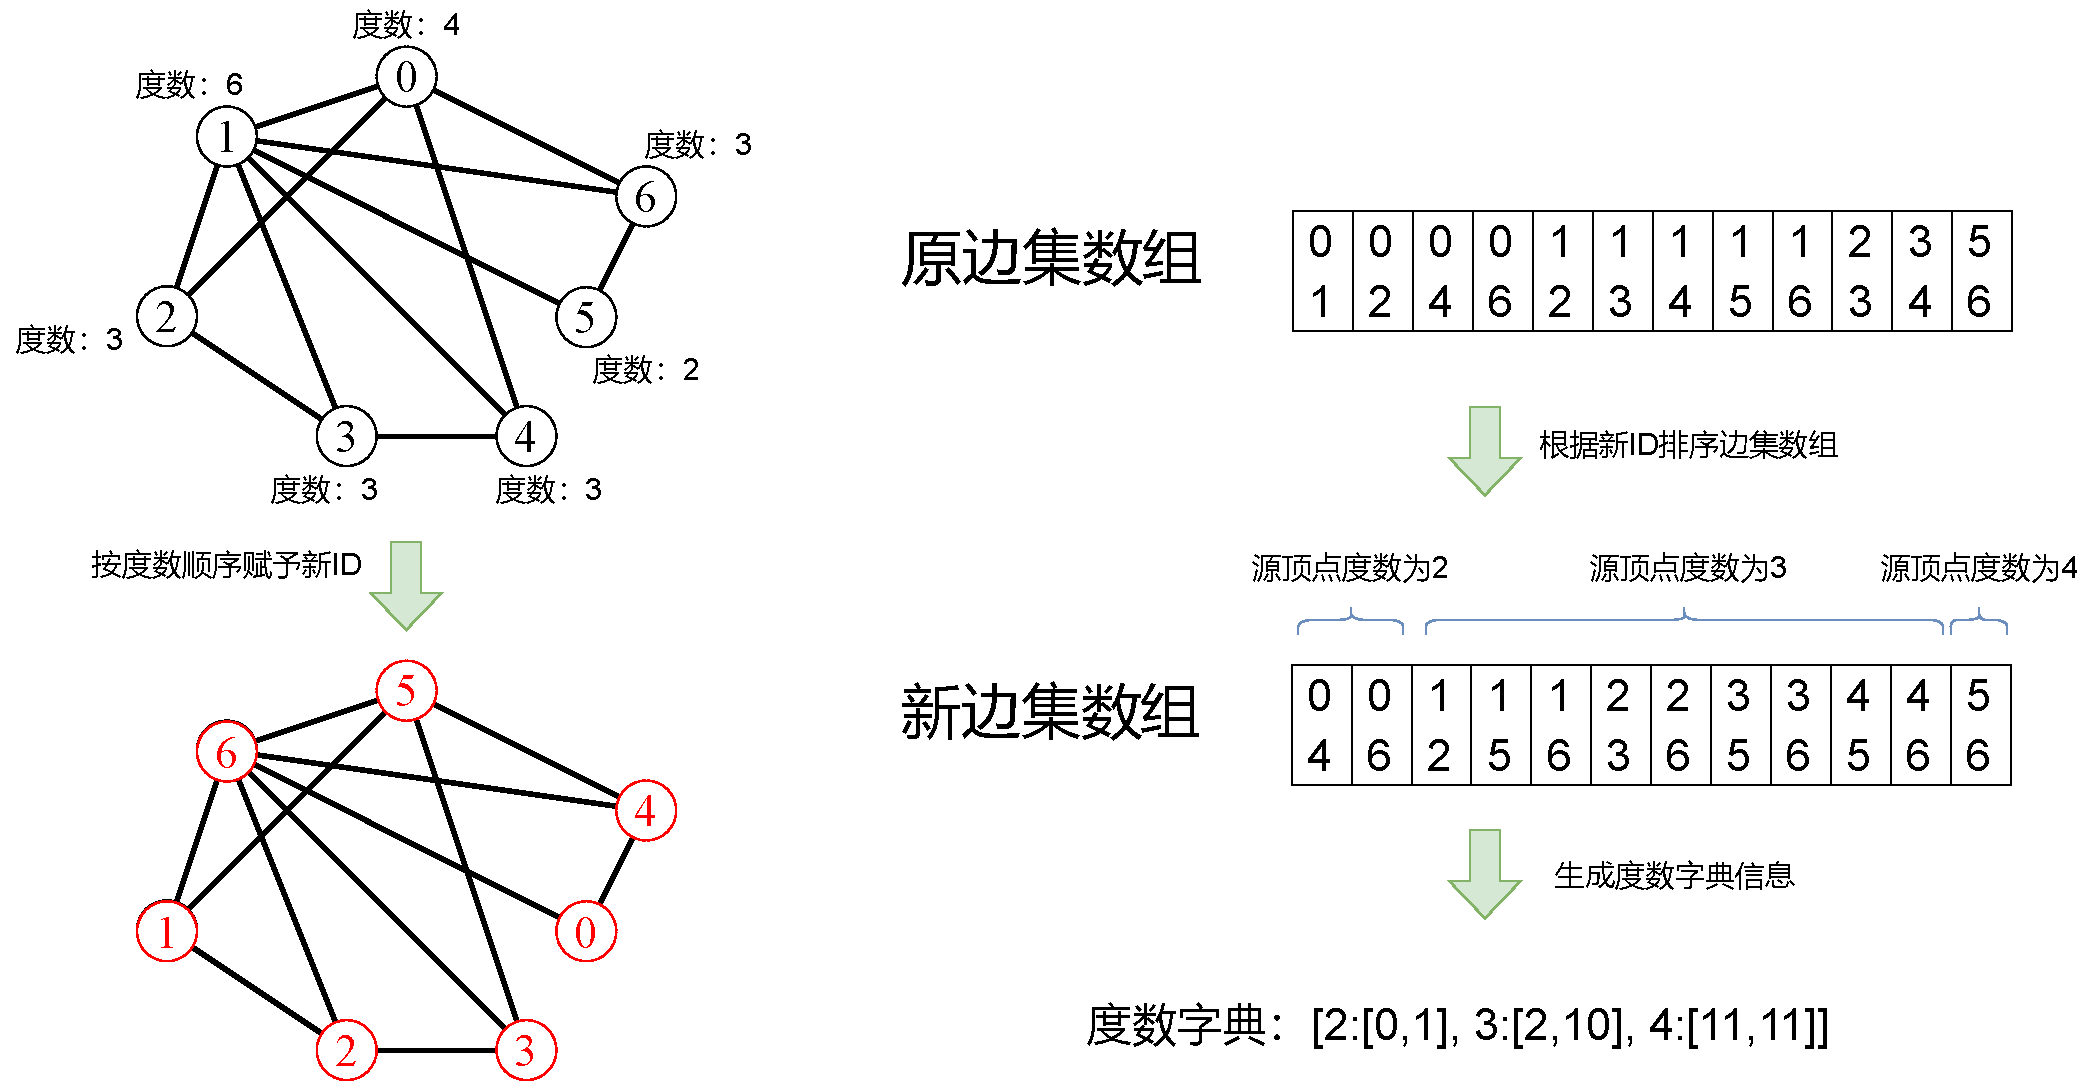
\includegraphics[width=\linewidth]{pic/degree_dic.pdf}
    \caption{度数重排序和度数字典}
    \label{fig:degree-dic}
\end{figure}

    参考章节\ref{subsec:neighbor},邻域采样核心思想是将边集数组视为流,在已采样边的后续邻域中继续采样。理论上,边集数组
中排序靠后的边有更多次机会被采样到。度数重排序使得顶点度数大的边排序靠后,使得邻域采样算法能够以更高概率采样到模式。
以在\ref{fig:degree-dic}的图中进行三角形计数为例,未排序原图中顶点度数最大的边为$(0,1)$,形成三个三角形
$(\Delta(0,1,2),\Delta(0,1,4),\Delta(0,1,6))$,多于其他边。邻域采样第一步是从边集数组中均匀随机采样一条边$l_0$,
则采样到$l_0=(0,1)$的概率是$\frac{1}{12}$,从$l_0$的邻域采样到边$l_1=(0,2) or (0,4) or (0,6)$时,能够从后续边流中发现第三条边
形成三角形,所以三个三角形被发现的概率是$p=\frac{1}{12}*\frac{3}{8}\approx3.12\%$。

\begin{figure}
    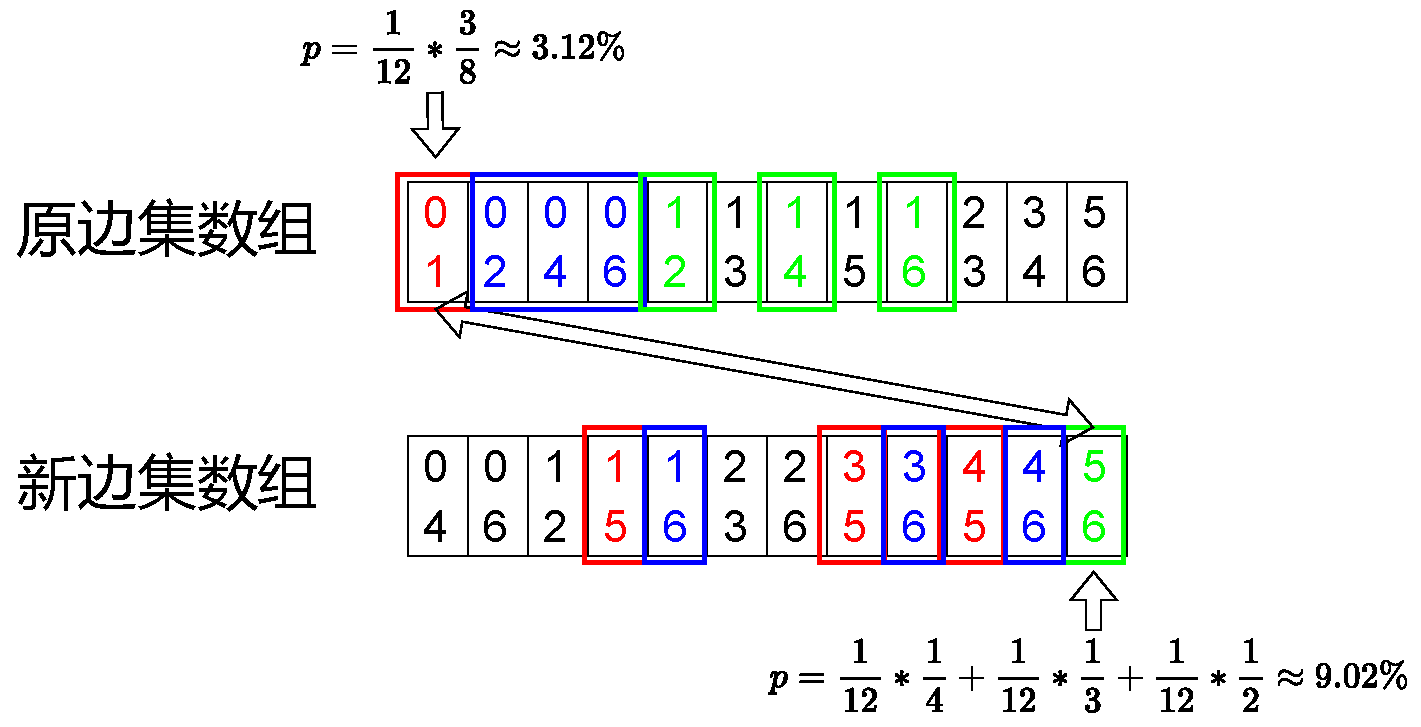
\includegraphics[width=\linewidth]{pic/reorder_pro.pdf}
    \caption{度数重排序后三角形计数被发现的概率}
    \label{fig:reorder_pro}
\end{figure}
    
    如图进行度数重排序后,边$(0,1)$对应的边为$(5,6)$,排序在边集数组末尾,三角形为$(\Delta(1,5,6),\Delta(3,5,6),\Delta(4,5,6))$

共有三种情况能够发现三个三角形,分别是:$l_0=(1,5),l_1=(1,6)$、$l_0=(3,5),l_1=(3,6)$、$l_0=(4,5),l_1=(4,6)$。三个三角形被发现
的概率是$p=\frac{1}{12}*\frac{1}{4}+\frac{1}{12}*\frac{1}{3}+\frac{1}{12}*\frac{1}{2}\approx9.02\%$。大约是重排序前的三倍,
在更大的数据集中这个差距将会更加显著。

\subsection{度数字典生成}
\label{subsec:deg-dic}
    模式分布模型构建模块需要将图数据划分为度数子图。本文将度数子图定义为某一度数的所有顶点及其连接边构成的子图。如何快速地
从图数据集中划分出度数子图是一个关键问题。如果直接在边集数组中划分度数子图,需要遍历计算所有顶点的度数,然后获取某一范围内
的所有顶点及其连接边,过程耗时较长,因此在预处理模块中对图数据集进行生成度数字典,加速划分度数子图。

    如图\ref{fig:degree-dic}所示,根据已经重排序的边集数组生成度数字典,字典以key-value形式存储源顶点度数相同边在边集
数组中的位置信息:key为度数,value为该度数的边的起止位置。在划分度数子图时,使用度数字典可以快速查找到某个度数相关边在
边集数组中的起止位置,从而得到该度数子图的边集。

\subsection{压缩稀疏行索引生成}
\label{subsec:csr}
    作为模式采样估计模块基础的邻域采样算法需要对边集数组进行遍历。在预处理阶段对边集生成压缩稀疏行索引,保存每个顶点的邻
域信息,可以加速遍历操作。

\begin{figure}
    \subfloat[输入图]{
        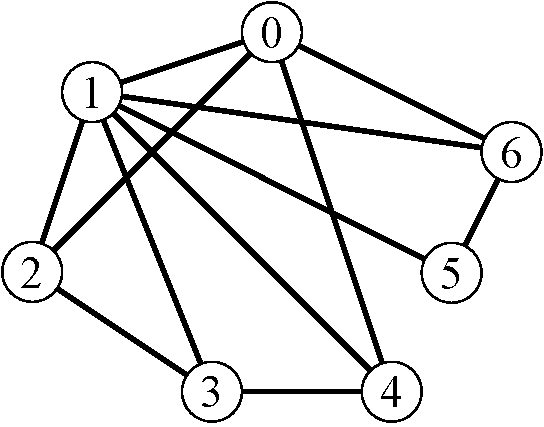
\includegraphics[width=.3\linewidth]{pic/csr_graph_example.pdf}
        \label{pic:input-graph}
    }
    \subfloat[压缩稀疏行索引]{
        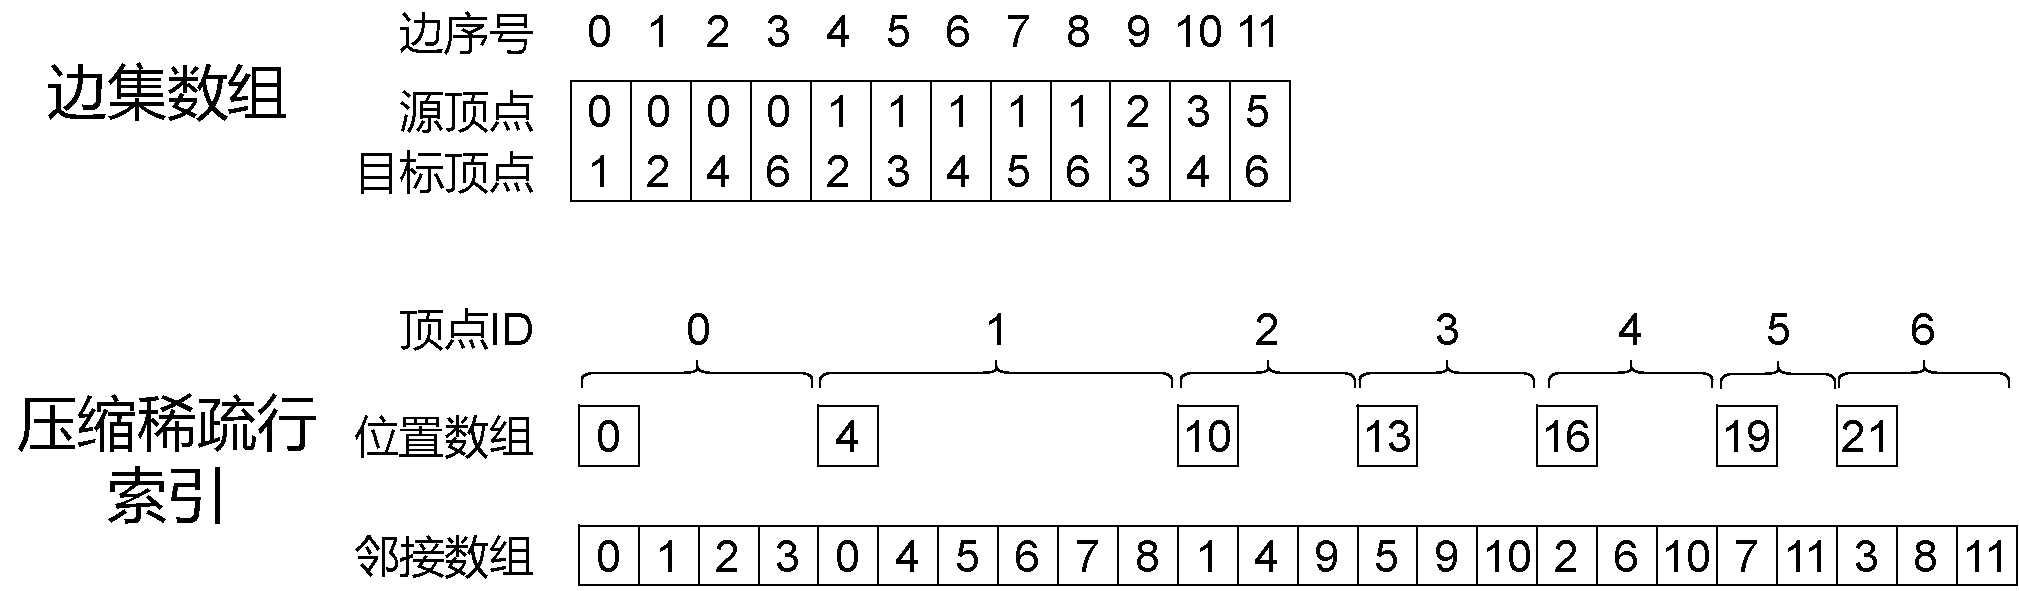
\includegraphics[width=.6\linewidth]{pic/csr_array.pdf}
        \label{pic:csr}
    }
    \caption{生成压缩稀疏行索引示例}
    \label{fig:gen-csr}
\end{figure}
    在图\ref{fig:gen-csr}中作为例子的输入图是一个无向图$G(V,E)$,它的存储为一个边集数组。边集数组数组经过排序,保证
$(SrcID,DstID)$升序排列。压缩稀疏行索引由两个一维数组组成。
\begin{itemize}
    \item 位置数组。存储了每个顶点的所有连接边中的第一条边在索引数组中的起始位置。位置数组的下标就是输入图中所有
    顶点的ID,因此不需要额外存储顶点ID相关信息,可以按照ID在数组中直接寻址。也因此位置数组大小应为输入图的顶点数。
    \item 索引数组。存储了每一条边在边集数组中的序号。这些边按照顶点顺序进行存储,即先存储顶点0到的所有连接边,
    再存储顶点1的所有连接边,以此类推。其中每一条边都会在$(SrcID,DstID)$两个顶点的连接边中出现,将会被存储了两次,因此
    索引数组的大小应该是边集数组的两倍。
\end{itemize}
    在压缩稀疏行索引中可以很快速地根据顶点ID信息找到所有ID的连接边,而不用在原始的边集数组中搜索每条边的顶点来获得连接边。
邻域采样算法中,关键思想是在已采样边的所有连接边中继续采样,因此会在边集数组中遍历搜索两个顶点来发现连接边。本文利用压缩
稀疏行索引优化采样过程。下面介绍使用压缩稀疏行索引的邻域采样算法。

\begin{figure}
    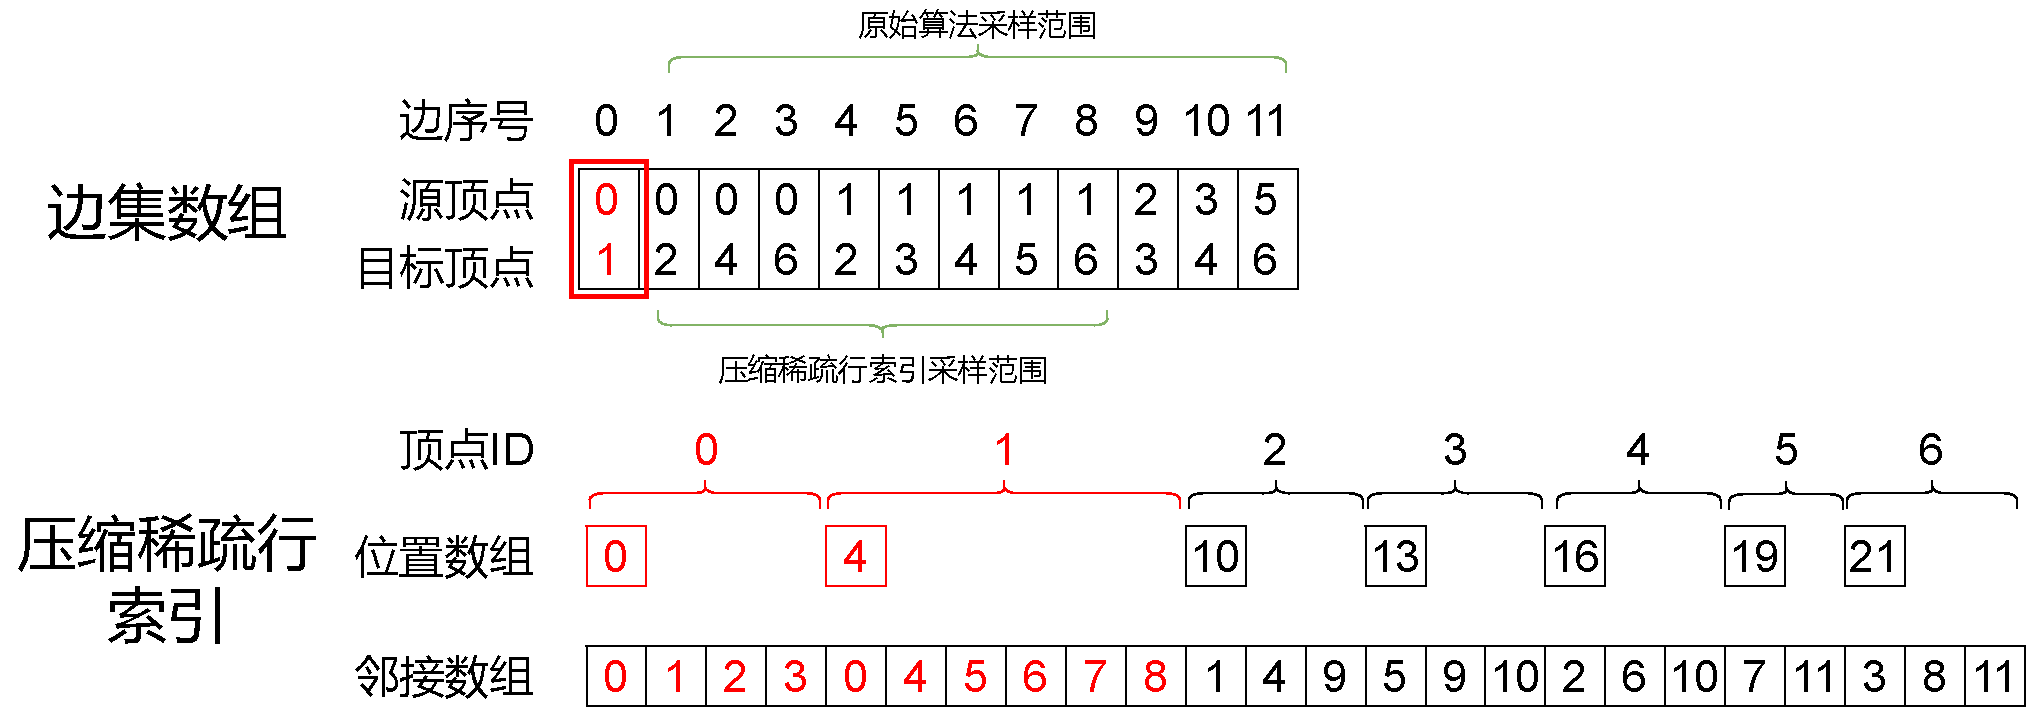
\includegraphics[width=.7\linewidth]{pic/sample_use_csr.pdf}
    \caption{使用压缩稀疏行从连接边中采样}
    \label{fig:samp_use_csr}
\end{figure}

    以三角形估计为例,在邻域采样算法中的第一步是在边集数组中均匀随机采样一条边,在这一步骤中不需要使用压缩稀疏行索引,
因此保持跟原本算法不变。而在采样第二条边时,如图\ref{fig:samp_use_csr}所示,假设在采样到第一条边$l_0$是边集中序号为
$0$的边$(0,1)$,邻接采样算法将边视为流,如果不使用压缩稀疏行索引,将会在边集数组的后续边中搜索顶点$0$和顶点$1$的邻接
边。而引入压缩稀疏行索引之后,直接从压缩稀疏行索引中查询对应的连接边序号,然后从中剔除序号小于等于$0$的边得到连接边。

\begin{figure}
    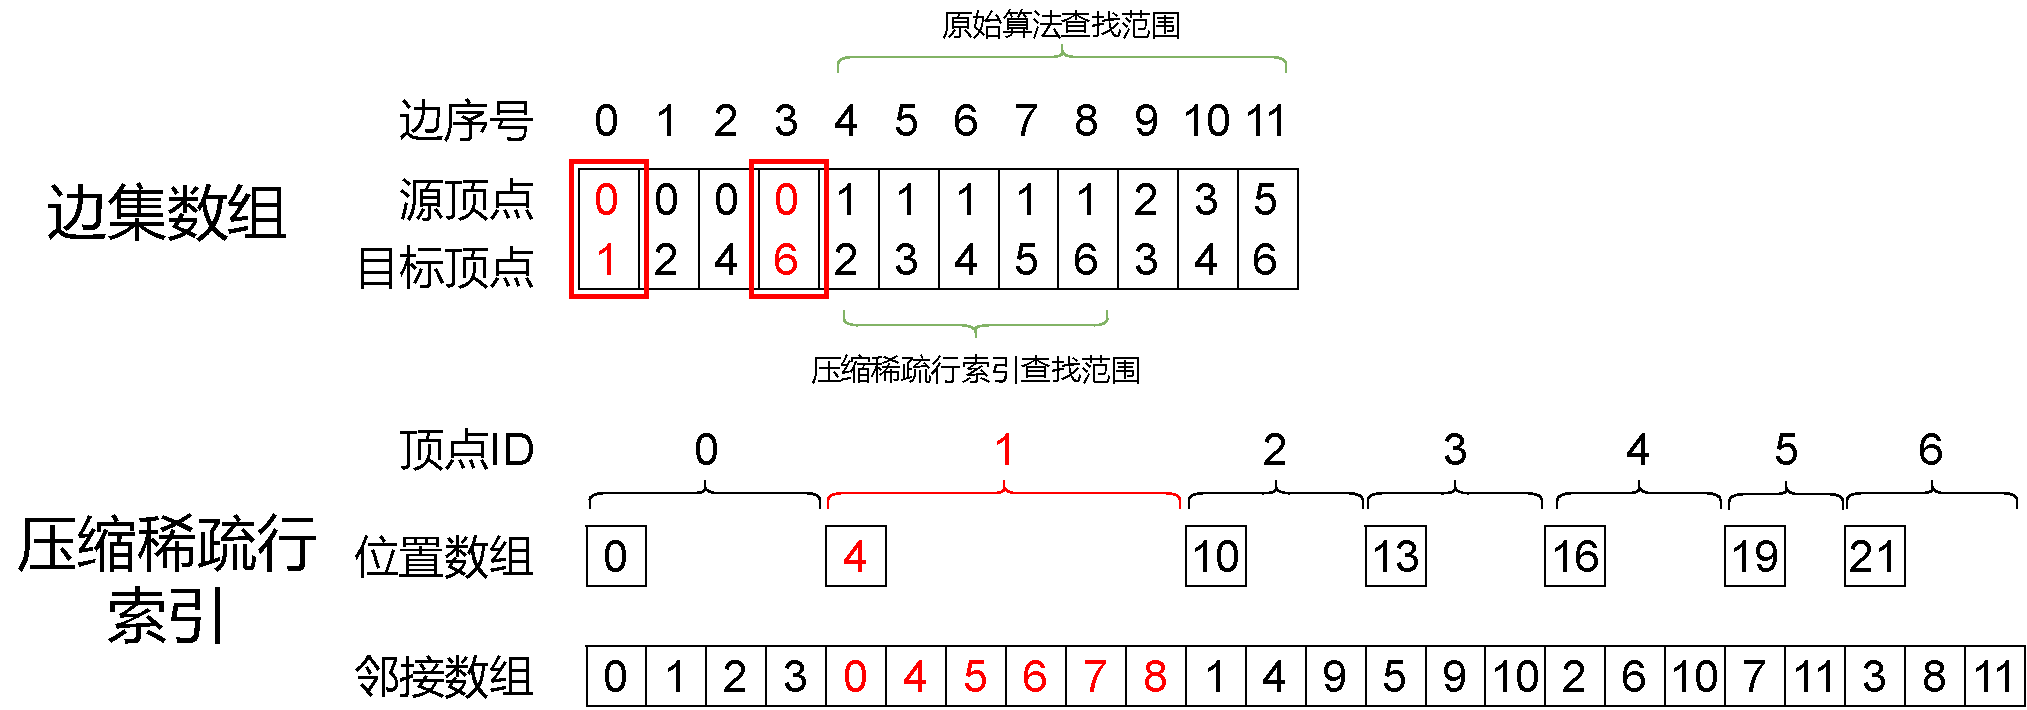
\includegraphics[width=.7\linewidth]{pic/check_use_csr.pdf}
    \caption{使用压缩稀疏行查找最后一条边}
    \label{fig:check_use_csr}
\end{figure}

    假设在连接边中采样的第二条边$l_1$是序号为$3$的边$(0,6)$,在最后一步需要查找是否存在能够形成三角的边$(1,6)$。同理,使用
压缩稀疏行索引可以快速判断顶点$1$的连接边中包含边$(1,6)$,可以构成三角形。

\section{模式采样模块设计}
\label{sec:sampling-module}

    模式采样模块的基础是邻域采样算法,根据\ref{sec:pow-law-analysis}中的观察,对图数据集进行区域划分,将采样偏向于高度数区
域,提高采样精度。并提供一种在误差和执行时间的权衡技术。本节描述该模块的设计要点。
    
\subsection{区域划分策略}
\label{subsec:partition}
    在近似计算中,分层采样是处理歪斜数据的常用方法。幂律图也是歪斜数据的一种,体现为少量高度数顶点拥有大量连接边,也贡献了大量的
模式。因此在本文利用分层采样的思想,根据顶点度数将图数据划分为两个区域。划分方法是收集高度数顶点其连接边形成子图。本文将这部分由
高度数顶点及其连接边形成的子图称为高度数区域,剩余顶点和连接边的子图则称为低度数区域。划分区域的目的是使采样更集中于高度数区域。

    本文采用边切法法进行划分区域,即将图的边分配到各子图中时,如果边的两个顶点各自属于不同的子图则将边复制后同时分配给两个子图。
边切分会造成边的冗余。

\begin{figure}
    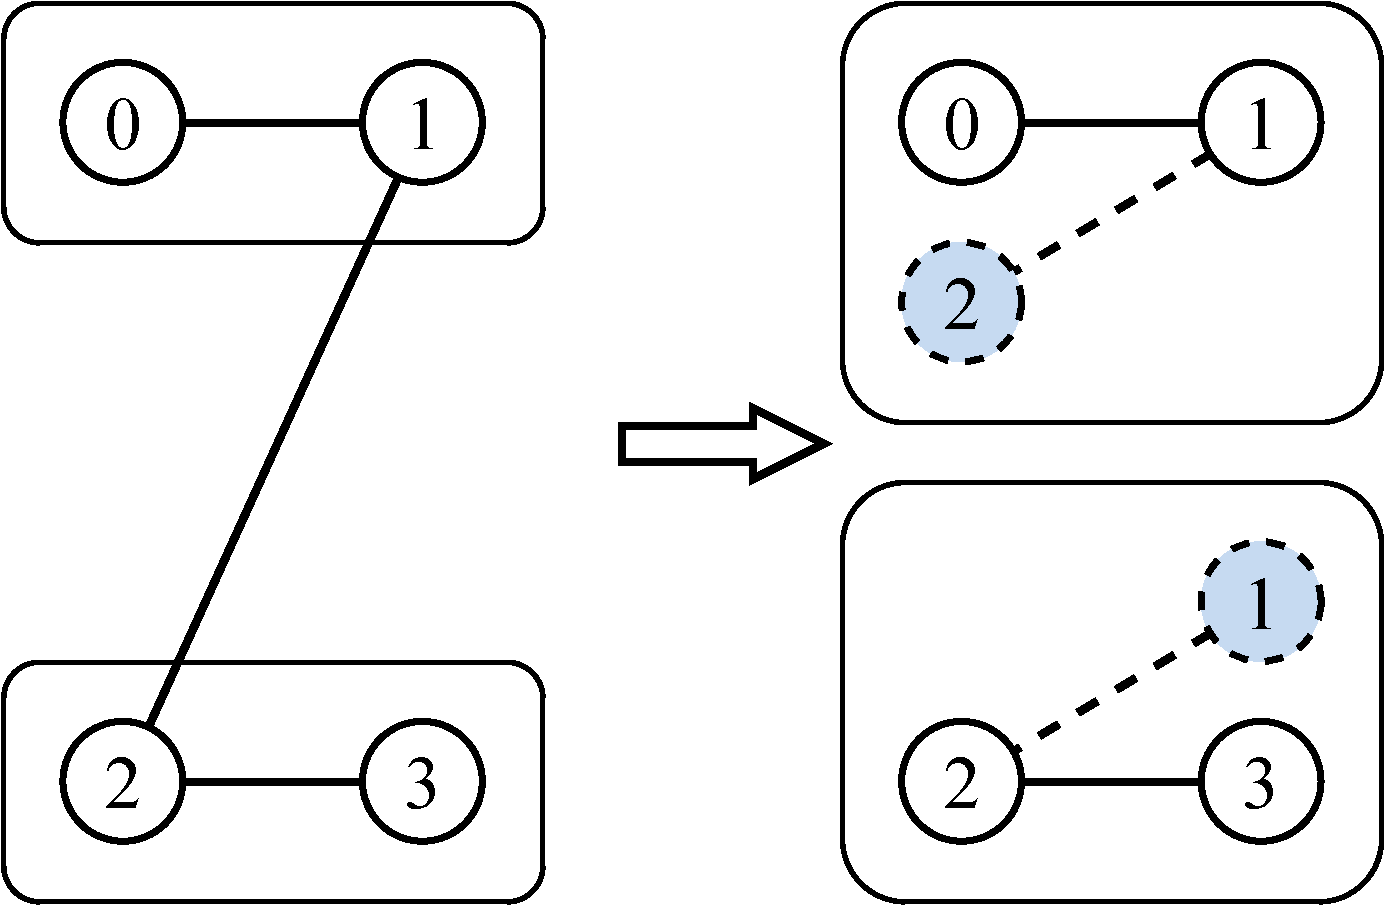
\includegraphics[width=.5\linewidth]{pic/cut.pdf}
    \caption{边切分法}
\end{figure}

    划分区域时,一个重要的问题是如何决定高度数区域的大小。本文以高度数区域占原边集数组的比例作为衡量指标,测试了多个数据上的区域
划分估计效果,并于原始邻域采样估计效果进行了对比。在图\ref{fig:partition}中可以看出高度数区域如果占据原图的绝大多数边或者极少数
边,估计误差较大,中间部分误差普遍较小。根据该观察,本文直觉地选择高度数区域占50\%作为本文模式采样算法正式执行时的区域划分标准。
\begin{figure}[h]
    \centering
    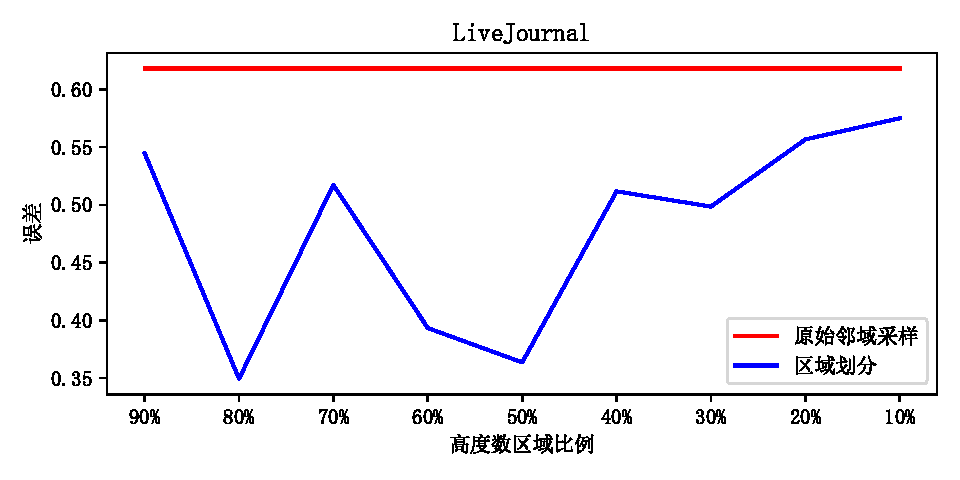
\includegraphics[width=0.5\linewidth]{pic/partition/LiveJournal.pdf}%
    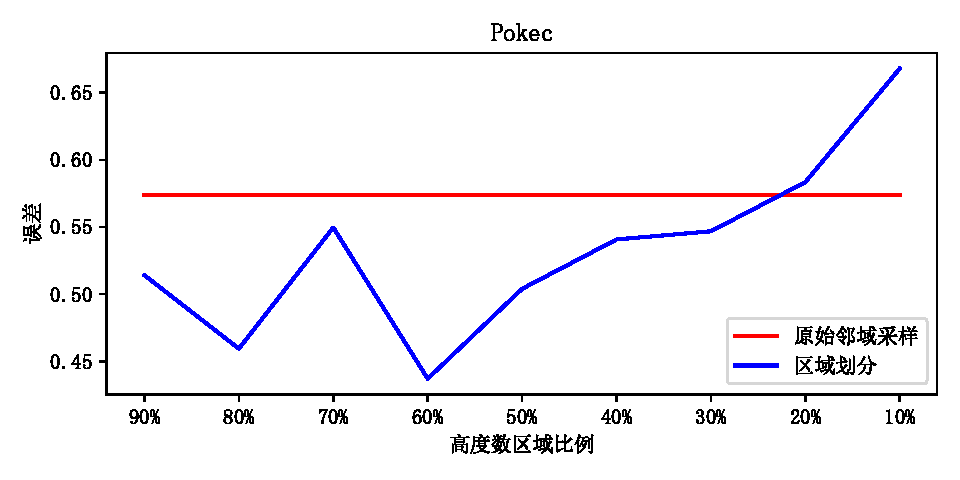
\includegraphics[width=0.5\linewidth]{pic/partition/Pokec.pdf}\\
    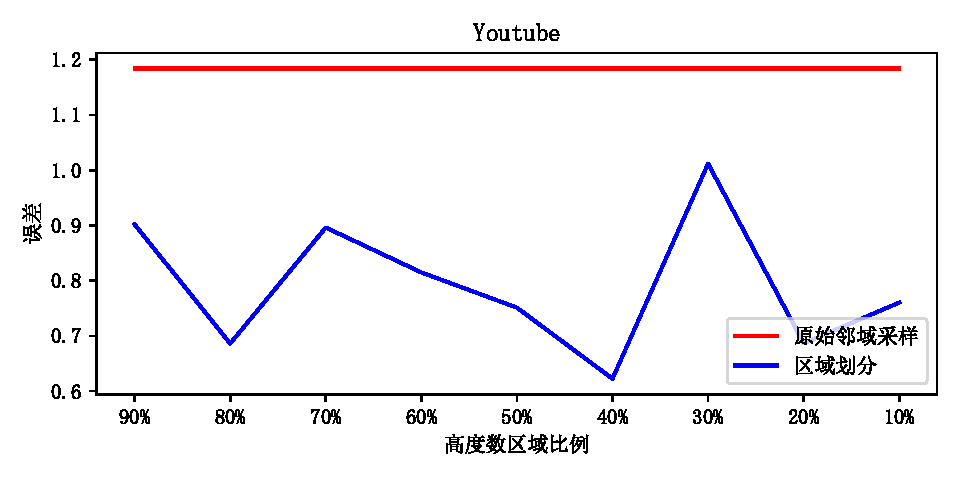
\includegraphics[width=0.5\linewidth]{pic/partition/Youtube.pdf}%
    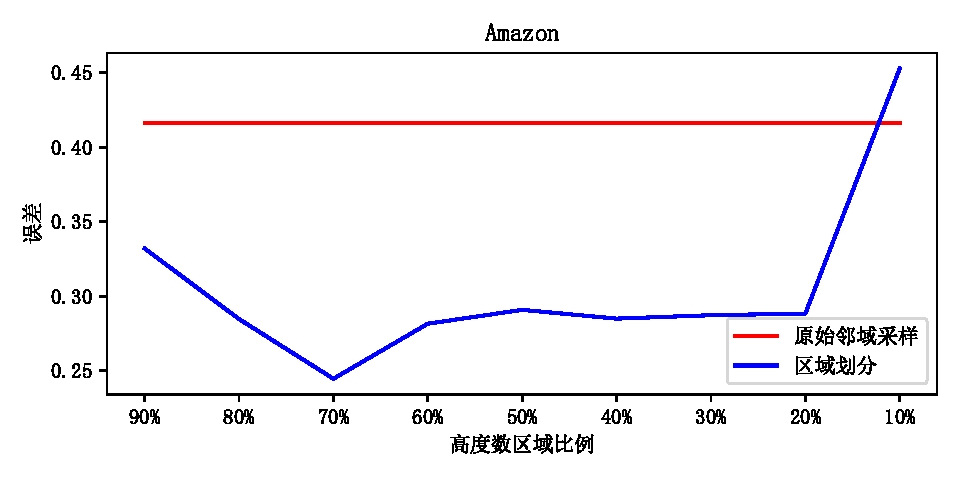
\includegraphics[width=0.5\linewidth]{pic/partition/Amazon.pdf}\\
    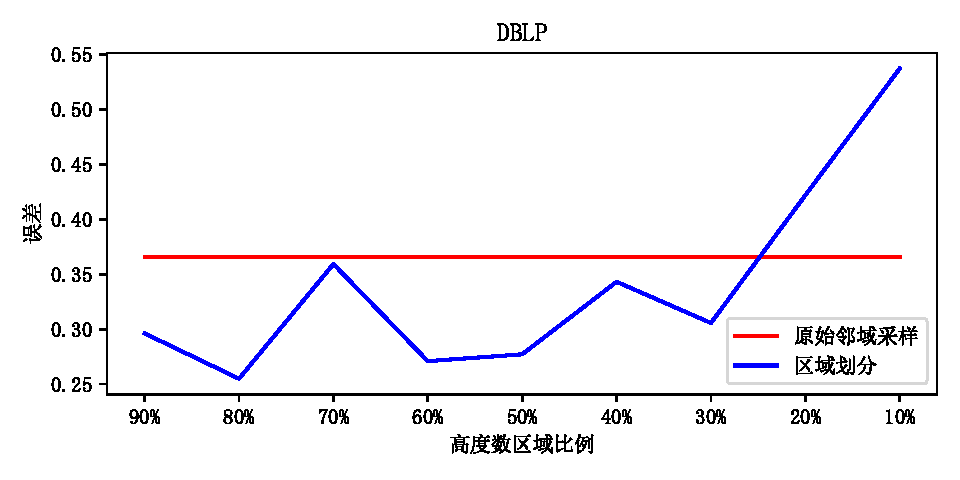
\includegraphics[width=0.5\linewidth]{pic/partition/DBLP.pdf}%
    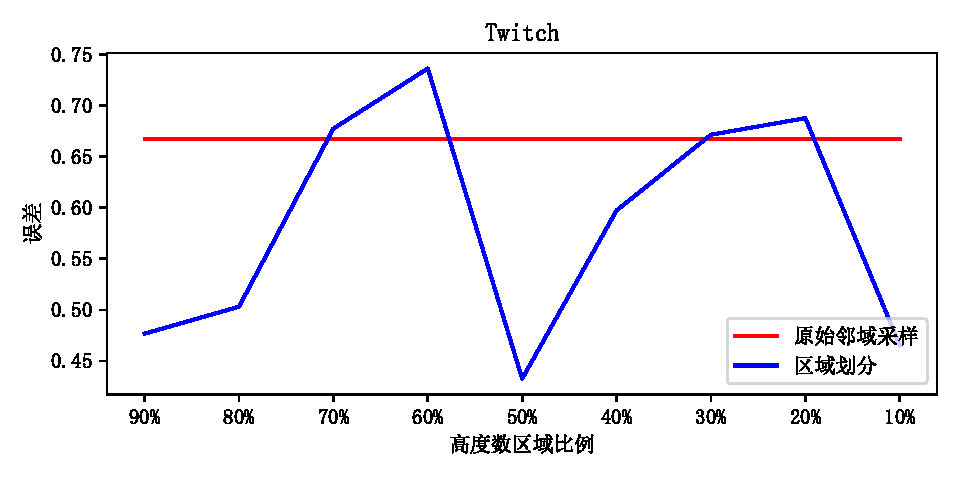
\includegraphics[width=0.5\linewidth]{pic/partition/Twitch.pdf}\\
    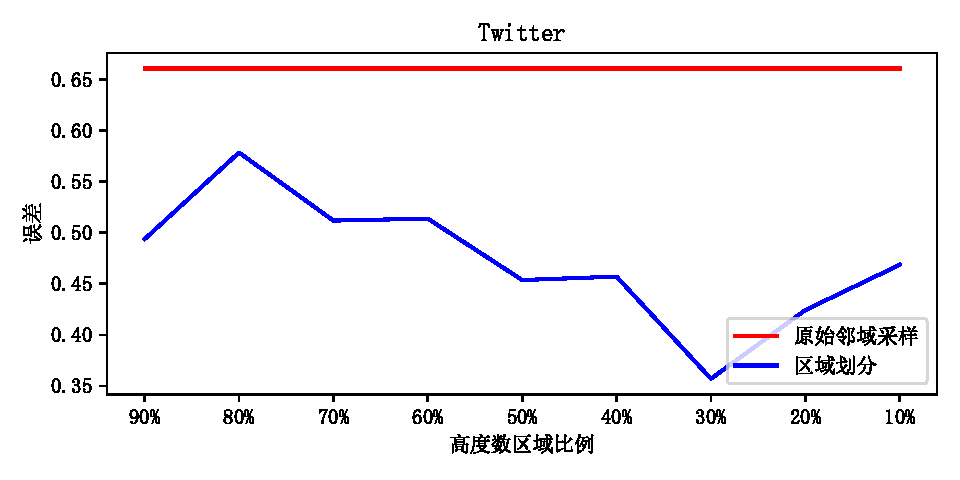
\includegraphics[width=0.5\linewidth]{pic/partition/Twitter.pdf}%
    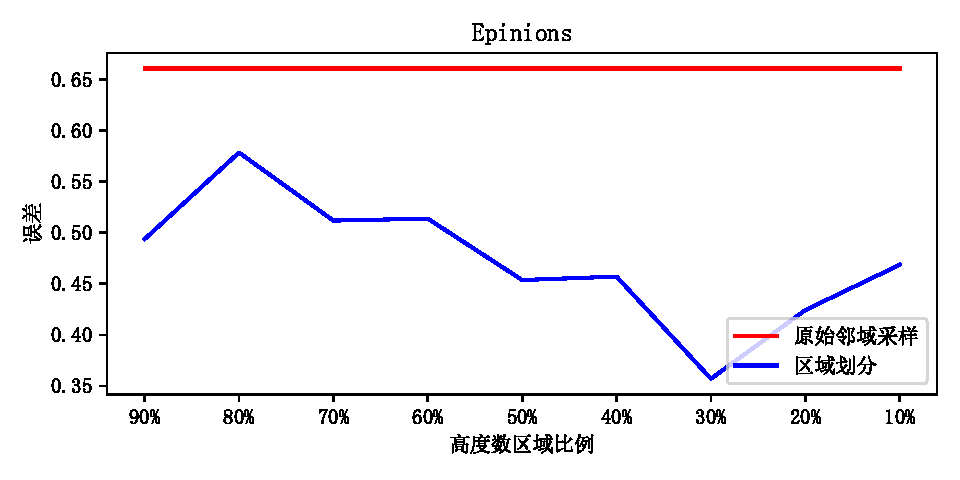
\includegraphics[width=0.5\linewidth]{pic/partition/Epinions.pdf}\\
    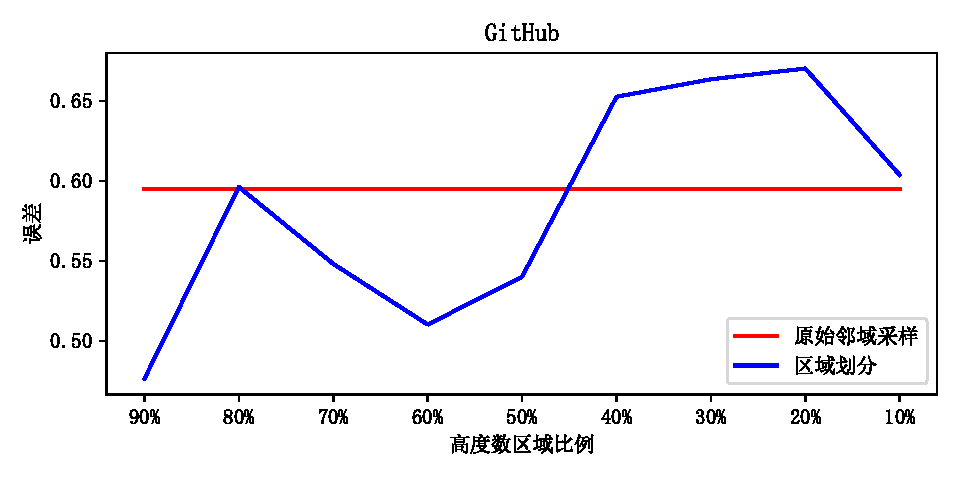
\includegraphics[width=0.5\linewidth]{pic/partition/GitHub.pdf}%
    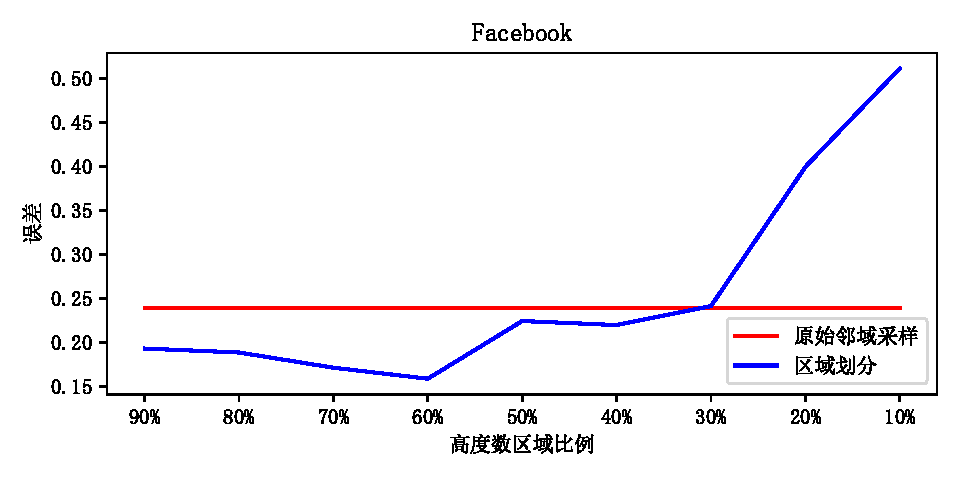
\includegraphics[width=0.5\linewidth]{pic/partition/Facebook.pdf}
    \caption{区域划分估计误差}
    \label{fig:partition}
\end{figure}

    划分区域后,优先按照上述比例为高度数区域分配估计器。由于有部分冗余边同时存在于两个区域,两个区域边总数大于原
边集数组,按照比值分配给高度数区域后,剩余估计器分配给低度数区域,数量将不满足其边数与原边集数组比值。上述分配方法使得在相同估计器
数量下,相对更集中于在高度数区域采样,同时没有忽略低度数区域采样。
    
\subsection{估计器数量选择策略}
\label{subsec:elp}
    许多近似计算系统都有着执行时间越长误差越低的特点,这些系统往往都会追求更加准确,但如果执行时间过长,将大大降低系统的可用性。
甚至某些极端情况下,执行时间比精确计算还要长但误差却难以降至0,近似系统得不偿失。因此如何在执行时间和执行时间和误差之间进行权衡,
是每个近似计算系统都需要考虑的问题。本文提出的系统执行基于邻域采样优化的模式采样算法,执行时间和误差根据估计器数量进行平衡,估计
器数量越多,算法所需要的执行时间越长,误差越低。

\begin{figure}[t]
    \centering
    \subfloat[时间与估计器数量]{
        \includegraphics[width=0.49\linewidth]{pic/estNum/time.pdf}
        \label{fig:rela-tn}
    }
    \subfloat[误差与估计器数量]{
        \includegraphics[width=0.49\linewidth]{pic/estNum/error.pdf}
        \label{fig:rela-en}
    }
    \caption{时间、误差与估计器数量的关系}
\end{figure}

    根据观察,对于一个给定的图数据集和一个模式,算法的执行时间与估计器数量线性相关。与之不同的是,误差与估计器非线性相关:
    在估计器数量较少的时候,随着估计器数量增加误差迅速下降,当估计器数量达到一
定程度,误差几乎不再变得更小。

    系统可以根据用户输入指定执行时间或者误差来选择估计器数量。

\begin{enumerate}
    \item[(1)] 指定时间选择估计器数量。如图\ref{fig:rela-tn}所示不同数据集的执行时间与估计器。
    数量近似斜率不同的直线。选择几组少量的估计器测试执行时间,并使用线性回归拟合测试结果与估计器数量的线性关系。另外
    估计器数量较少时容易受其他因素影响(如硬件cpu线程数等)并不完全是线性关系,为了更好的拟合直线,应倾向于当估计数较少时收集更多的点来减少
    误差,而当估计数增加时收集更少的点。获得关系直线后根据用户输入的执行时间从该直线中获得合适的估计器数量。

    \item[(2)] 指定误差选择估计器数量。图\ref{fig:rela-en}中显示误差与估计器数量的关系接近指数函数。由于误差需要预先得知模式挖掘的准确结果
    才能进行计算,上述通过少量估计器测试后进行拟合的方法难以直接运用。因此本文采用另一种方法进行推断。首先对原数据集的边集进行均匀随机
    采样,将规模缩小到可以直接通过精确计算算法得到结果而运行时间非常短暂,在实践中,发现将采样规模保持在10\%左右可以满足这一点。然后再小图上
    执行精确算法,并用多组少量估计器测试误差。接着根据误差测试结果拟合误差与估计器数量曲线。
    
    \item[(3)] 未指定直接选择估计器数量。在用户未指定时,根据上述(2)中方法构造误差与估计器数量曲线,由于执行时间与估计器数量几乎呈线性关系,
    所以不需要额外构造(1)中的直线。然后直接根据曲线选择误差为0.05对应的估计器数量,保证估计误差在0.05以内。

\end{enumerate}

\section{模式分布模型构建模块}
\label{sec:fitting-module}
    模式分布模型构建模块通过获取部分度数子图的模式数量作为数据点,使用非线性回归拟合\ref{sec:pow-law-analysis}中的模式累积分布曲线。
根据曲线估算模式总数。本节描述该模块的设计要点。

\subsection{部分度数子图采样策略}
\label{subsec:deg-sub-samp}
    为了拟合模式累积分布曲线,需要选择一些度数子图作为样本,然后计算每个样本的模式数量。可以在每个度数子图上运行准确的算法进行模式计数,
但有时在使用邻域采样快速地在度数子图上进行估计也是可以接受的。本文将前一种方法称为准确方法,后一种方法称为近似方法。系统允许用户自由
决定选择哪种方式进行计算。为了更好的准确度,应选择准确方法,而为了快速估计,则应选择近似方法。

    一个关键的问题是选择哪些度数子图作为样本。为了拟合累积分布曲线,需要计算模式数的累加和,准确方法和近似方法采用不同的方式。准确方法中,
计数$d+1$度子图的模式时,只计算所有$d+1$度顶点新增的模式数量,与之前已有的模式数累加作为样本数据点。近似方法中,则将所有$d+1$度顶点的连接边加入到$d$度
子图中形成新的度数子图,新的度数子图包含所有$d+1$及以下度数的顶点,然后在子图上执行邻域采样算法估计模式数直接作为样本数据点。
因此,本文从度序列的起始度数提取连续的子序列作为样本。之后的挑战是如何确定样本子序列的长度。这实际上是采样开销和拟合精度之间的权衡。

\begin{figure}[t]
    \centering
    \subfloat[长度:15\%,误差:102.25\%,时间:1.1s]{%
      \includegraphics[width=0.49\linewidth]{pic/select-length/com-amazon-1.pdf}}\hfill
    \subfloat[长度:25\%,误差:50.57\%,时间:3.2s]{%
      \includegraphics[width=0.49\linewidth]{pic/select-length/com-amazon-2.pdf}}\hfill
    \subfloat[长度:35\%,误差:26.64\%,时间:5.6s]{%
      \includegraphics[width=0.49\linewidth]{pic/select-length/com-amazon-3.pdf}}\hfill
    \subfloat[长度:45\%,误差:18.83\%,时间:10.4s]{%
      \includegraphics[width=0.49\linewidth]{pic/select-length/com-amazon-4.pdf}}
    \caption{不同样本子序列长度下的拟合误差和执行时间。长度分别为15\%、25\%、35\%和45\%度数占比。}
    \label{fig:sample-length}
\end{figure}

    图\ref{fig:sample-length}显示了不同样本序列长度对Amazon数据集的影响。很明显,序列越长,结果越准确。然而,
考虑到计算开销和误差的权衡,25\%是更好的选择。对于不同的图数据集,合适的样本子序列长度是不同的,本文通过一种启发式方法来进行选择。

    基于\ref{fig:sample-length}所示。模式累积分布曲线是一条凸曲线,在低度数部分快速上升,然后保持相当长的平尾。
为了精确地拟合曲线,最好保持足够的低度数数据点,直到“转折点”后曲线开始变平缓。在曲线快速上升的部分斜率逐渐减小,理论上,
转折点是斜率突然下降到接近0的度数。因此从最小度数开始模式计数,并计算度数斜率,直到度数达到阈值。以此方式来确定样本子序列长度。
通常采样的顶点只占整个数据集的一部分。此外,系统也允许用户直接设置样本子序列长度。

    选择样本子序列以后,需要计算每个度数子图的模式数。首先由于近似方法下估计计数的方差较大,斜率阈值设置应小于准确方法下的斜率阈值,
而由于近似方法比准确方法快得多,即使选择更大的样本子序列长度也可以接受。
    
    \begin{figure}[t]
        \centering
        \includegraphics[width=.7\linewidth]{pic/error.pdf}
        \caption{顶点3和顶点6随着新度数添加到采样的度数子图时,三角$\Delta(3,A,B),\Delta(3,B,6)$需要通过缩放因子$f$进行估算。}
        \label{fig:error}
      \end{figure}

    在近似方法下得出的模式计数会出现遗漏,需要进行调整与准确方法中的计数保持一致。如图\ref{fig:error}所示,只有顶点都出现在采样的
度数子图中的三角形才能计数,如$\Delta(1,2,3), \Delta(2,5,6)$,但那些越过边界的三角形将被忽略,如$\Delta(3,A,B)和\Delta(3,B,6)$。
因此通过“缩放因子”$f$对近似方法的模式数进行调整。假设采样的度数子图中的总边数和剩余子图边数分别为$a$和$b$,则度数子图中一个
模式的所有边被采样的概率(即模式可以被扫描的概率)为$\left(\frac{a}{a+b}\right)^K$,其中$K$是模式的边数。同理,该概率在剩余子图
为$\left(\frac{b}{a+b}\right)^K$。如果近似方法找到$n$个三角形,则考虑越过边界的三角后估计实数为等式5,因此缩放因子为$f=(|E|^K-b^K)/a^K$,其中$|E|=a+b$。

\begin{equation}
  \label{eq:scaling-factor}
  \begin{split}
    n' &= \frac{n}{\left(\frac{a}{a+b}\right)^K} \cdot \left(1-\left(\frac{b}{a+b}\right)^K\right)\\
       & = n\cdot \frac{(a+b)^K-b^K}{a^K} = n\cdot \frac{|E|^K-b^K}{a^K}
  \end{split}
\end{equation}

\subsection{拟合累积分布曲线}
\label{sec:fit-formula}
    获得样本子序列的模式数作为数据点后,可以进行非线性回归拟合累积分布曲线。根据\ref{subsec:deg-sub-samp}中的描述,
大多数样本来自低度数部分,很少来自高度数部分,因此曲线的尾部可能拟合不好,导致拟合误差很大。为了解决这一潜在问题,
本文采用了两种技术来增强采样数据:样本加权和样本插值。

    样本插值主要是在样本的末尾部分进行插值。图的度数通常是非连续的,特别是在高度部分,度数分布非常稀疏。因此对数据
点进行线性插值,补充没有出现的度数,将主要增加的是高度数的样本数量。这在一定程度上增加了高度数的权重,这些高度数样本
位于转折点附近,对曲线形状有重大影响,使得拟合曲线尾部将更接近真实值。准确方法的样本的末端部分相对平坦,在曲线中比较稳定,
因此可以安全地对缺失的度数进行插值。默认情况下不对近似方法的样本进行插值。这是由于近似方法得出的样本并不准确,对于某些数
据集,高度样本非常分散,需要过多的插值点,将放大近似方法本身引入的误差。

\section{本章小结}
    本章描述了对图数据集的幂律分析的重要观察,主要包括:模式集中于高度数顶点连接边;模式的累积分布呈幂律特性。基于以上观察
设计了基于幂律属性的模式近似挖掘系统整体架构。架构分为三个部分:预处理模块、模式采样估计模块、模式分布模型构建模块。其中
预处理模块在加载图数据时对图数据集进行预先处理,帮助后续模式挖掘任务。模式采样估计模块执行邻域采样优化的算法,将采样集中在
高度数顶点连接边提高采样精度。模式分布模型构建模块使用少量样本数据拟合模式累积分布曲线。

\chapter{系统实现}

\section{预处理模块实现}
\label{sec:preprocessing-impl}

    预处理模块中首先通过Apache Spark GraphX加载图数据集。图数据集往往规模较大,以文件的形式存储于磁盘中,GraphX提供了
GraphLoader类加载磁盘中的图数据文件。GraphLoader类中加载接口函数为edgeListFile,从边列表格式的文件中加载图数据,文件
每行包含两个整数:源顶点id和目标顶点id。GraphLoader将加载的图数据组织为Graph类,Graph类将顶点存储为Vertex,将边存储
为Edge,允许访问顶点和边及其底层结构相关联的属性。

    Graph类及其关联的Vertex和Edge主要结构如表\ref{tab:class-graph},加载时顶点和边的属性值默认为NULL,系统的模块主要通过
Graph类对顶点和边进行操作。
\begin{table}
    \caption{Graph[VD,ED]}
    \begin{tabular}{|c|c|c|}
     \hline
     变量 & 数据类型 & 含义\\
     \hline
     vertices &  Array[Vertex[VD]] & 存储顶点ID及相关属性值的集合\\
     edges & Array[Edge[ED]] &存储边的两端顶点ID及相关属性值的集合\\
    \hline
    \end{tabular} 
    \label{tab:class-graph}
\end{table}

\begin{table}
    \caption{Vertex[VD]}
    \begin{tabular}{|c|c|c|}
     \hline
     变量 & 数据类型 & 描述\\
     \hline
     id &  Long & 顶点ID\\
     attr & VD & 可自定义类型的顶点属性\\
     \hline
    \end{tabular} 
    \label{tab:class-vertex}
\end{table}

\begin{table}
    \caption{Edge[ED]}
        \begin{tabular}{|c|c|c|}
        \hline
        变量 & 数据类型 & 描述\\
        \hline
        srcId &  Long & 源顶点ID\\
        dstId &  Long & 目标顶点ID\\
        attr & ED & 可自定义类型的边属性\\
        \hline
        \end{tabular} 
    
    \label{tab:class-edge}
\end{table}
    
    加载图数据后,首先执行简单化去除自环和平行边,然后进行度数重排序使边集数组按照顶点度数排列,接着根据排序后边集数组并行地
生成度数字典和压缩稀疏行索引。流程如图\ref{fig:preprocess-flow}所示。
\begin{figure}
    \centering
    \includegraphics[width=.7\linewidth]{pic/preprocess_flow.pdf}
    \caption{预处理流程}
    \label{fig:preprocess-flow}
\end{figure}


\subsection{图简单化实现}
\label{subsec:simplification-impl}

    简单化模块主要为了去除图中的自环和平行边。通过遍历边集数组寻找平行边和自环。对于自环,边的两个顶点ID相同即可删除。
同时维护一个邻接表,在表中查询每条边是否已经存在,存在则删除。主要相关变量如表\ref{tab:class-simp}
    \begin{table}
        \caption{图简单化相关变量}
        \resizebox{\textwidth}{!}{
            \begin{tabular}{|l|l|l|}
            \hline
            变量 & 数据类型 & 描述\\
            \hline
            edges &  Array[Edge] & Graph中原始边集\\
            adj &  Map[Long, Set[Long]] & 邻接表,key是边的srcId,value是源顶点是srcId的所有边的dstId的集合\\
            \hline
            sEdges &  Array[Edge] &  简单化边集,去除了平行边和自环\\
            \hline

            \end{tabular} 
        }
        \label{tab:class-simp}
    \end{table}


\begin{algorithm}[H]
    \KwData{$edges$}
    \KwResult{$adj$,$sEdges$}
    \For{$e$ in $edges$}{
        \If{$e.srcId = e.dstId$}{
            remove $e$ from $edges$
        }
        \Else(){
            \If(){$e.dstId$ $\in$ $adj[e.srcId]$}{
                remove $e$ from $edges$
            }
            \Else(){
                insert $e.dstId$ to $adj[e.srcId]$\\
                insert $e.srcId$ to $adj[e.dstId]$\\
            }
        }
    }
    $sEdges$ $\leftarrow$ $edges$\\
    \Return{$adj$, $sEdges$}
    \caption{图简单化伪代码}
    \label{alg:simplification}
\end{algorithm}

    算法\ref{alg:simplification}生成的邻接表adj去除了自环和平行边,并且adj还将在后续的度数重排序模块中使用。

\subsection{度数重排序实现}
\label{subsec:degree-sort-impl}
    度数重排序通过上一节\ref{subsec:simplification-impl}生成的邻接表adj计算每个顶点的度数,利用度数对
adj中的原本的顶点oldId进行排序,将排序后的下标作为newId。然后遍历修改Graph类的顶点集vertices和边集edges。
由于GraphX的Vertex类和Edge类允许自定义属性,因此使用属性来存储度数信息。
\begin{table}
    \caption{度数重排序相关变量}
    \resizebox{\textwidth}{!}{
        \begin{tabular}{|l|l|l|}
        \hline
        变量 & 数据类型 & 描述\\
        \hline
        vertices &  Array[Edge] & Graph中原始顶点集\\
        sEdges &  Array[Edge] & 简单化边集\\
        adj &  Map[Long, Set[Long]] & 邻接表,用于统计顶点度数,并作为中间变量存储旧id对应的新id\\
        \hline
        rVertices &  Array[Edge] & 重排序顶点集\\
        rEdges &  Array[Edge] & 重排序边集\\
        radj & Map[Long, Long]  & 重排序后顶点和度数的映射表\\
        \hline
        \end{tabular} 
    }
    \label{tab:class-reorder}
\end{table}

\begin{algorithm}
    \KwData{$adj$, $vertices$, $sEdges$}
    \KwResult{$rVertices$, $rEdges$, $rAdj$}
    \tcc{每个顶点的连接边数即度数作为顶点的属性}
    \For{$v$ in $vertices$}{
        $v.attr$ $\leftarrow$ sizeof($adj[v.id]$)
    }
    sort $vertices$ with attr \\
    $rVertices$ $\leftarrow$ $vertices$\\
    
    \For(\tcc{根据排序后$vertices$下标i改写新id,并建立旧id和新id以及度数间的映射}){$i$ $\leftarrow$ 0 To sizeof($vertices$)}{
        $v.id$ $\leftarrow$ $i$\\
        $adj[vertices[i].id]$ $\leftarrow$ $(i, vertices[i].attr)$\\
    }
    
    \For(\tcc{改写$edges$的$srcId$和$dstId$,保证$srcId < dstId$。顶点度数作为边的属性}){$e$ in $edges$}{
        \If{$e.srcId < e.dstId$}{
            $e.srcId$ $\leftarrow$ $adj[e.srcId].newId$\\
            $e.dstId$ $\leftarrow$ $adj[e.dstId].newId$\\
            $e.attr$ $\leftarrow$ $(adj[e.srcId].degree, adj[e.dstId].degree)$\\
        }
        \Else(){
            $e.srcId$ $\leftarrow$ $adj[e.dstId].newId$\\
            $e.dstId$ $\leftarrow$ $adj[e.srcId].newId$\\
            $e.attr$ $\leftarrow$ $(adj[e.dstId].degree, adj[e.srcId].degree)$\\
        }
    }
    sort $edges$ with $srcId$ and $dstId$\\
    $rEdges$ $\leftarrow$ $edges$\\
    
    \For(\tcp{生成新顶点id和度数的映射表}){$n$ in $adj$}{
        $rAdj[n.newId]$ $\leftarrow$ $n.degree$
    }
    \Return{$rVertices$, $rEdges$, $rAdj$}
    \caption{度数重排序伪代码}
    \label{alg:degree-reorder}
\end{algorithm}

    经过度数重排序后得到按度数升序排列顶点集vertices和边集edges,顶点和边的属性存储了度数信息,将用于生成度数字典。
另外,记录了新顶点ID和度数的映射表将使用于压缩稀疏行索引的生成。

\subsection{度数字典实现}
\label{subsec:deg-dic-impl}
    遍历已排序后的边集,根据边的属性生成度数字典,标注不同度数的边在排序边集中的位置。

\begin{table}
    \caption{度数字典相关变量}
    \resizebox{\textwidth}{!}{

    \begin{tabular}{|l|l|l|}
        \hline
        变量 & 数据类型 & 描述\\
        \hline
        rEdges &  Array[Edge] & 重排序边集\\
        \hline
        dicDegree &  Map[Long, (Long, Long)] & 度数字典,key为度数,value为该度数边在rEdges中的起止位置\\
        \hline

    \end{tabular} 
    }
    \label{tab:class-degree-dic}
\end{table}

\begin{algorithm}[H]
    \KwData{$rEdges$}
    \KwResult{$dicDegree$}
    $begin$ $\leftarrow$ 0
    $end$ $\leftarrow$ 0
    
    \For(\tcp{遍历边集,收集不同度数边的起止位置下标}){$i$ $\leftarrow$ 0 to sizeof($rEdges$)}{

         \If(){$rEdges[i].attr \neq rEdges[i-1].attr$}{
            $dicDegree[rEdges[i-1].attr]$ $\leftarrow$ $(begin , end)$\\
            $begin$ $\leftarrow$ $i$
         }
         \Else{
            $end$ $\leftarrow$ $i$
         }
    }
    \Return{dicDegree}
    \caption{度数字典伪代码}
    \label{alg:degree-dic}
\end{algorithm}

\subsection{压缩稀疏行索引实现}
\label{subsec:csr-impl}
    压缩稀疏行索引由位置数组和索引数组组成。首先,顶点和度数的映射表反应了每个顶点的连接边数,因此可以通过该映射表确定
每个顶点相邻边集的起始位置序号。接着,扫描边集数组,根据边的srcId和dstId将边的序号插入到索引数组中,过程中需要通过
offsets数组记录每个顶点边集的插入位置。
\begin{table}
    \caption{压缩稀疏行索引相关变量}
    \resizebox{\textwidth}{!}{
    \begin{tabular}{|l|l|l|}
        \hline
        变量 & 数据类型 & 描述\\
        \hline
        rAdj & Map[Long, Long]  & 重排序后顶点和度数的映射表\\
        rEdges &  Array[Edge] & 重排序边集\\
        \hline
        offsets & Array[Long] & 每个顶点边集的插入位置,长度为顶点数,初始值全为0,随着边插入而增加\\
        \hline
        positions &  Array[Long] & 位置数组,长度为顶点数,每个顶点在csrIndexes中起始位置序号\\
        csrIndexes &  Array[Long] & 索引数组,每条边在rEdges中的位置序号\\
        \hline
    \end{tabular} 
    }
    \label{tab:class-csr}
\end{table}

\begin{algorithm}[H]
    \KwData{$rAdj$,$rEdges$}
    \KwResult{$positions$, $csrIndexes$}
    $positions[0]$ $\leftarrow$ 0\\
    \For(){$i$ $\leftarrow$ 1 to $max(rAdj.keys)$}{
        $positions[i]$ $\leftarrow$ $rAdj[i-1].degree + positions[i-1]$\\
        $offsets[i]$ $\leftarrow$ 0\\
    }
    \For(){$i$ $\leftarrow$ 0 to sizeof($rEdges$)}{
        $insertSrc$ $\leftarrow$ $positions[rEdges[i].srcId] + offsets[rEdges[i].srcId]++$\\
        $insertDst$ $\leftarrow$ $positions[rEdges[i].dstId] + offsets[rEdges[i].dstId]++$\\
        $csrIndexes[insertSrc]$ $\leftarrow$ $i$\\
        $csrIndexes[insertDst]$ $\leftarrow$ $i$\\
    }
    \Return{$positions$, $csrIndexes$}
    \caption{压缩稀疏行索引伪代码}
    \label{alg:csr}
\end{algorithm}

\section{模式采样估计模块实现}
\label{sec:sampling-impl}
    依据\ref{sec:sampling-module}中的设计,模式采样估计模块对传统邻域采样算法进行优化,对边集数组进行高低度数区域划分,并且
提供估计器选择策略。同时,本文使用的\ref{subsec:csr}中压缩稀疏行索引加速邻域采样算法的遍历过程。本文实现了压缩稀疏行
索引版本的邻域采样核心算法,在此基础上实现了估计器选择和区域划分。然后将估计器总数量按照边数比例分配到高低度数区域,并发地启动估计。
最终以所有估计器的平均值作为估计结果。整体流程如图\ref{fig:sample-flow}所示。
\begin{figure}
    \centering
    \includegraphics[width=.7\linewidth]{pic/sample_flow.pdf}
    \caption{模式采样估计流程}
    \label{fig:sample-flow}
\end{figure}

\subsection{邻域采样核心算法实现}
\label{subsec:nei-core}

\begin{table}
    \caption{Estimator接口结构}
    \resizebox{\textwidth}{!}{
            \begin{tabular}{|l|l|l|}
            \hline
            类型 & 名称 & 描述 \\
            \hline
            \multirow{5}{*}{变量} & Array[Edge] edges                                                    & 图数据的边集数组      \\
            & Array[Long] position                                                 & 压缩稀疏行索引中的位置数组 \\
            & Array[Long] csrIndexes                                               & 压缩稀疏行索引中的索引数组 \\
            & Long curIdx                                                             & 当前采样边的位置      \\
            & Array[Edge] sampledEdges                                             & 已经采样的边集       \\
            \hline
            \multirow{4}{*}{函数} & sample() $\rightarrow$ (Edge e, Double p)                                & 均匀随机采样边集数组一条边 \\
            & neighborSample(Array[Edge] sampled) $\rightarrow$ (Edge e, Double p) & 均匀随机采样邻域一条边   \\
            & close(Array[Edge] unsampled) $\rightarrow$ Bool isClose                  & 搜索未采样边是否会出现  \\
            & mining() $\rightarrow$ Long count                                      & 执行模式挖掘,不同模式重写该函数  \\
            \hline

            \end{tabular} 
        }
    \label{tab:class-est}
\end{table}

    本文将邻域采样算法的主要采样估计过程抽象为表\ref{tab:class-est}中的接口Estimator,Estimator体现了使用邻域采样
进行近似模式挖掘的主要三个阶段:
\begin{itemize}
    \item \textbf{sample}。均匀随机的采样边集数组中的一条边,边集数组的大小为$l$,采样每条边的概率$p=\frac{1}{l}$。
    输出采样到的边$e$和采样概率$p$。具体实现中,sample步骤直接在边集数组中采样,不需要使用压缩稀疏行索引。

    \item \textbf{neighborSample}。输入已经采样到的所有边,从边集数组中搜索已采样的邻域边,从中均匀随机采样一条边,
    邻域大小为$c$,采样概率为$p=\frac{1}{c}$,输出采样到的边$e$和采样概率$p$。原始的邻域采样算法中,根据已采样边搜索邻域
    的过程非常昂贵,需要遍历边集数组,本文具体实现中使用压缩稀疏行索引收集顶点邻域边,加速搜索。

    \item \textbf{close}。当已采样边覆盖模式的所有顶点时,输入模式的未采样边,在边集数组的后续邻域中搜索为采样边是否出现。
    与neighborSample相同,具体实现通过压缩稀疏行索引加速搜索过程。
\end{itemize}

    伪代码\ref{alg:sample}、\ref{alg:nei-sample}、\ref{alg:close}显示了采用压缩稀疏行索引加速的邻域采样算法具体实现。

\begin{algorithm}[H]
    \KwResult{$e$, $p$}
    $l$ $\leftarrow$ sizeof($edges$)\\
    $curIdx$ $\leftarrow$ Random 0 to $l$\\
    \Return{$edges(curIdx)$, $\frac{1}{l}$}
    \caption{sample伪代码}
    \label{alg:sample}
\end{algorithm}

\begin{algorithm}[H]
    \KwData{$sampled$}
    \KwResult{$e$, $p$}
    $sampledVertex$ $\leftarrow$ $\emptyset$\\
    \For{e in sampled}{
        insert $e.srcId$ into $sampledVertex$\\
        insert $e.dstId$ into $sampledVertex$\\
    }
    $neighbors$ $\leftarrow$ $\emptyset$\\
    \For(){$v$ in $sampledVertex$}{
        \For{$idx$ in $csrIndexes[positions[v]..positions[v+1]-1]$ and $idx > curIdx$}{
            insert $idx$ into $neighbors$
        }
    }
    $l$ $\leftarrow$ sizeof($neighbors$)\\
    $neiIdx$ $\leftarrow$ Random 0 to $l$\\
    $curIdx$ $\leftarrow$ $neighbors[neiIdx]$\\
    \Return{$edges(curIdx)$, $\frac{1}{l}$}
    \caption{neighborSample伪代码}
    \label{alg:nei-sample}
\end{algorithm}

\begin{algorithm}[H]
    \KwData{$unsampled$}
    \KwResult{$e$, $p$}
    $isClose$ $\leftarrow$ \ForAll{$e$ in $unsampled$}{
        $v$ $\leftarrow$ $e.srcId$\\
        $u$ $\leftarrow$ $e.dstId$\\
        exist $idx$ in $csrIndexes[positions[v]..positions[v+1]-1]$ satisfy $idx > curIdx$ and $edges[idx].dstId = u$\\
        }
    \Return{$isClose$}
    \caption{close伪代码}
    \label{alg:close}
\end{algorithm}

    系统中实现了常见的几种模式的挖掘算法:2-链(长度为2的路径)、三角形和4-团(4个顶点的完全连通图),继承了Estimator接口
生成ChainEstimator、TriangleEstimator类和CliqueEstimator,并且重载实现了各自的mining函数。如\ref{alg:chain-est}、
\ref{alg:tri-est}、\ref{alg:clique-est}所示,不同模式结构的具体实现细节有区别:ChainEstimator中进行sample、neighborSample
而不需要执行close;TriangleEstimator两次采样后通过close判断第三条边是否存在;CliqueEstimator要根据前三条边是否构成三角来决定
再次执行neighborSample还是执行close。对于更多的模式结构,系统允许用户通过继承Estimator接口来开发不同的挖掘算法。
开发不同的模式挖掘算法。

\begin{algorithm}[H]
    \KwResult{$count$}
    $(e0, p0)$ $\leftarrow$ sample()\\
    $(e1, p1)$ $\leftarrow$ neighborSample($e0$)\\
    \tcp{采样$e0$时无法确定剩余顶点的id,采样$e1$后则不需要close步骤}
    \uIf{!e1}{
        \Return{0}
    }
    \Else{
        \Return{$\frac{1}{p0*p1}$}
    }
    \caption{ChainEstimator.mining伪代码}
    \label{alg:chain-est}
\end{algorithm}

\begin{algorithm}[H]
    \KwResult{$count$}
    $(e0, p0)$ $\leftarrow$ sample()\\
    $(e1, p1)$ $\leftarrow$ neighborSample($e0$)\\
    \If(){!e1}{
        \Return{0}
    }
    \tcp{搜索三角形中剩余的那一条边}
    $unsampled$ $\leftarrow$  triangle - $(e0, e1)$\\
    \uIf{close($unsampled$)}{
        \Return{$\frac{1}{p0*p1}$}
    }
    \Else{
        \Return{0}
    }
    \caption{TriangleEstimator.mining伪代码}
    \label{alg:tri-est}
\end{algorithm}

\begin{algorithm}[H]
    \KwResult{$count$}
    ($e0$, $p0$) $\leftarrow$ sample()\\
    ($e1$, $p1$) $\leftarrow$ neighborSample($e0$)\\
    \If(){!e1}{
        \Return{0}
    }
    ($e2$, $p2$) $\leftarrow$ neighborSample($(e0, e1)$)\\
    \If(){!$e2$}{
        \Return{0}
    }
    $unsampled$ $\leftarrow$ $\emptyset$\\
    \tcp{如果采样边形成三角形,已采样边缺少第四个顶点,还需要继续采样}
    \uIf{$(e0, e1, e2)$ is a triangle}{
        $(e3, p3)$ $\leftarrow$ neighborSample($(e0, e1, e2)$)
        \If(){!$e3$}{
            \Return{0}
        }
        $unsampled$ $\leftarrow$  Clique - $(e0, e1, e2, e3)$\\
        $p$ $\leftarrow$ $p0*p1*p2*p3$\\
    }
    \tcc{如果三条边没有形成三角形,则为长度3的链,包含了四个顶点,调用close}
    \Else{
        $unsampled$ $\leftarrow$  Clique - $(e0, e1, e2)$\\
        $p$ $\leftarrow$ $p0*p1*p2$\\
    }
    \uIf{close($unsampled$)}{
        \Return{$\frac{1}{p}$}
    }
    \Else{
        \Return{0}
    }
    \caption{CliqueEstimator.mining伪代码}
    \label{alg:clique-est}
\end{algorithm}

 
\subsection{区域划分实现}
\label{subsec:partition-impl}
    在\ref{subsec:partition}区域划分策略中,需要收集高度数顶点及其连接边形成高度数区域,剩余部分形成低度数区域。在具体实现中
利用压缩稀疏行索引进行划分。由于顶点id经过度数重排序,位置数组positions的按照顶点度数的升序排列,因此positions的末尾向前搜索
高度数顶点,通过csrIndexes获取该顶点的连接边添加到高度数区域,直到高度数区域边数占原边集数组50\%。

\begin{algorithm}[H]
    \KwData{$edges$, $positions$, $csrIndexes$}
    \KwResult{$hight$, $low$}
    \For{$i$ $\leftarrow$ sizeof($positions$) to 0}{
        \For(){$idx$ in $csrIndexes[positions[i]..positions[i+1]-1]$}{
            insert $edges[idx]$ into $hight$
        }
    }
    \For(){$idx$ in $csrIndexes[0..positions[i]]$}{
            insert $edges[idx]$ into $low$
    }
    \Return{$hight$, $low$}
    \caption{区域划分伪代码}
    \label{alg:patition}
\end{algorithm}
\subsection{估计器数量选择实现}
\label{subsec:elp-impl}
    在\ref{subsec:elp}中设计,系统根据用户指定执行时间或误差选择估计器数量。在实现中,用户通过重载Estimator接口确定模式结构,
估计器的数量体现为执行对应Estimator类的次数。

    用户指定执行时间$t$,为了在少量估计器时测试更多的数据点,采用指数间隔进行测试,从1个估计器开始逐次翻倍,直到数量达到1k。
测试后的数据通过调用scipy包的curve\_fit函数拟合直线$y = A*x+B$,拟合计算得出参数$A$、$B$,代入$t$计算估计器数量$n$。用户指定
误差$e$,首先通过GraphX提供的takeSample函数对边集以10\%的概率均匀随机采样生成小图,在小图上执行$[100,200,\ldots,1000]$
十组估计器测试误差,同样使用scipy包拟合曲线$y = A*(x+B)^K$,拟合计算得出参数$A$、$B$和$K$,代入$e$计算估计器数量$n$。
如果未指定
\begin{table}
    \caption{估计器选择调用主要函数}
    \resizebox{\textwidth}{!}{
            \begin{tabular}{|l|l|l|l|}
            \hline
            函数 & 参数 & 返回值 & 描述 \\
            \hline
            curve\_fit& \makecell[l]{callable f, Array data, Array p0}   & Array param & \makecell[l]{curve\_fit通过data拟合方程f,参数初始值设置为p0}      \\
            takeSample & Array data, Bool withReplacement, Double pro & Array sample & \makecell[l]{takeSample遍历data对其中每一个元素以pro概率采样,\\
                                                                                                        当withReplacement为true时进行有放回采样,否则无放回采样}\\
            \hline
            \end{tabular} 
        }
    \label{tab:elp-func}
\end{table}

\begin{algorithm}
    \KwData{$edges$, $input$}
    \KwResult{$n$}
    
    \uIf(\tcp{用户设置时间}){$input$ is time}{
        $t$ $\leftarrow$ $input$\\
        $data$ $\leftarrow$ $\emptyset$
        $n^*$ $\leftarrow$ 1
        \While(){$n^*$ < 1k}{
            $t^*$ $\leftarrow$ get runtime with $n^*$ * Estimators\\
            insert ($n^*$, $t^*$) into $data$\\
            $n^*$ $\leftarrow$ $2n^*$\\
        }
        $f$ $\leftarrow$ $(y = A*x + B)$\\
        \tcp{拟合直线$f$,初始参数设置$A = 1, B = 0$}
        $p$ $\leftarrow$ curve\_fit($f$, $data$, [1, 0]) \\
        set $f$ parameters use $p$\\
        $n$ $\leftarrow$ f$^{-1}$($t$)\\
    }
    \Else{
        \uIf(\tcp{用户设置误差}){$input$ is error}{
            $e$ $\leftarrow$ $input$
        }
        
        \Else(\tcp{未设置}){
            $e$ $\leftarrow$ 0.05
        }
        $data$ $\leftarrow$ $\emptyset$\\
        $smallGraph$ $\leftarrow$ takeSample($edges$, $false$, 10\%)\\
        \For(){$n^*$ in $[100,200,\ldots,1000]$}{
            $e^*$ $\leftarrow$ get error with $n^*$ * Estimators on $smallGraph$\\
            insert ($n^*$, $e^*$) into $data$\\
        }
        $f$ $\leftarrow$ $(y = A*(x+B)^K)$\\
        \tcp{拟合曲线$f$,初始参数设置$A = 1, B = 1, K = -1$}
        $p$ $\leftarrow$ curve\_fit($f$, $data$, [1, 1, -1]) \\
        set $f$ parameters use $p$\\
        $n$ $\leftarrow$ $f^{-1}(e)$\\
    }
    \Return{$n$}
    \caption{估计器选择伪代码}
    \label{alg:elp}
\end{algorithm}

\subsection{启动估计}
\label{subsec:launch}
    在进行了区域划分和决定了估计器数量之后启动估计。根据上述实现,调用一次Estimator接口的mining即执行了一次估计器,Estimator之间互不依赖
因此并发执行各估计器。启动时按照区域划分的边集占比分配估计器,所有估计器的估计结果求平均值作为整体估计结果。

\begin{algorithm}
    \KwData{$n$, $hight$, $low$}
    \KwResult{$pattern$}
    $hn$ $\leftarrow$ $\frac{sizeof(hight)}{sizeof(hight)+sizeof(low)}$ \\
    $ln$ $\leftarrow$ $\frac{sizeof(low)}{sizeof(hight)+sizeof(low)}$ \\
    $patterns$ $\leftarrow$ $\emptyset$\\
    parallel run $hn * Estimator(hight), ln * Estimator(low)$ and insert result into $patterns$\\
    \Return{$\frac{patterns}{n}$}
    \caption{启动估计伪代码}
    \label{alg:launch}
\end{algorithm}

\section{模式分布构建模块实现}
\label{sec:fitting-impl}
    根据\ref{sec:fitting-module}中的设计,模式分布构建模块利用度数字典划分度数子图,在度数子图上进行部分模式计数。模式分布构建模块
允许用户设置部分模式计数的具体方法:准确方法和近似方法。在部分模式计数的过程中判断样本数据的斜率是否小于用户设置阈值或者样本子序列是否
超过用户设置的长度,如果是则停止计数获得样本。根据样本进行曲线拟合。整体流程如图\ref{fig:fit-flow}。
\begin{figure}
    \centering
    \includegraphics[width=.7\linewidth]{pic/fit_flow.pdf}
    \caption{模式分布构建流程}
    \label{fig:fit-flow}
\end{figure}

\subsection{部分度数子图采样实现}
\label{subsec:fit-sample}
    度数字典记录了度序列中不同度数对应边在边集数组中的位置,遍历度数字典从边集数组中划分出对应的边集。用户选择准确方法或近似方法,采用不同方法计算:
准确方法在新度数的边集上执行精确的模式挖掘算法,并将得到的模式数与之前度数进行累加;近似方法将新度数的边添加到之前边集中,在新边集执行
度数子图的邻域采样算法。在\ref{sec:sampling-impl}的邻域采样算法中利用压缩稀疏行索引采样边集。原边集经过度数重排序,度数子图边集为原边集中连续的一部分
,因此根据度数子图的边集在压缩稀疏行索引中找出对应范围,针对每个度数子图建立度数范围数组。修改\ref{sec:sampling-impl}中算法,在查找压缩稀疏行
索引并采样的过程中根据度数范围数组限制采样范围。

\begin{table}
    \caption{部分度数子图采样主要数据结构}
    \resizebox{\textwidth}{!}{
            \begin{tabular}{|l|l|l|}
            \hline
            变量 & 类型 &  描述 \\
            \hline
            degreeRange& Array[Int]  & \makecell[l]{度数范围数组。压缩稀疏行索引中位置数组的表示\\
                                                    每个顶点对应边在索引数组中起始位置,\\
                                                    degreeRange则表示某个度数子图每个顶点的终止位置}   \\

            \hline
            \end{tabular} 
        }
    \label{tab:fit-samp-class}
\end{table}

    建立度数范围数组函数:

\begin{algorithm}
    \KwData{$range$, $positions$, $csrIndexes$}
    \KwResult{$degreeRange$}

    \For(){$i$ $\leftarrow$ 0 to sizeof($positions$)}{
        $degreeRange$[i] $leftarrow$ search $range$ in $csrIndexes[positions[i]..positions[i+1]]$
    }
    \Return{$degreeRange$}
    \caption{buildDegreeRange伪代码}
    \label{alg:build-degree-range}
\end{algorithm}

    根据度数范围数组限制采样范围的邻域采样算法:

\begin{algorithm}[H]
    \KwData{$sampled$, $degreeRange$}
    \KwResult{$e$, $p$}
    $\dots\dots$\\
    $neighbors$ $\leftarrow$ $\emptyset$\\
    \For(){$v$ in $sampledVertex$}{
        \tcp{在查找压缩稀疏行索引的过程中使用$degreeRange$限制范围}
        \For{$idx$ in $csrIndexes[positions[v]..degreeRange[v]]$ and $idx > curIdx$}{
            insert $idx$ into $neighbors$
        }
    }
    $\dots\dots$\\
    \Return{$edges(curIdx)$, $\frac{1}{l}$}
    \caption{度数子图neighborSample伪代码}
    \label{alg:nei-sample-range}
\end{algorithm}

\begin{algorithm}[H]
    \KwData{$unsampled$, $degreeRange$}
    \KwResult{$isClose$}
    $isClose$ $\leftarrow$ \ForAll{$e$ in $unsampled$}{
        $v$ $\leftarrow$ $e.srcId$\\
        $u$ $\leftarrow$ $e.srcId$\\
        \tcp{在查找压缩稀疏行索引的过程中使用$degreeRange$限制范围}
        exist $idx$ in $(csrIndexes[positions[v]..degreeRange[v]])$ satisfy $idx > curIdx$ and $edges[idx].dstId = u$\\
        }
    \Return{$isClose$}
    \caption{度数子图close伪代码}
    \label{alg:close-range}
\end{algorithm}

    在遍历度数字典的过程中,检测是否取得足够样本,依据用户设定,通过当前样本点数据计算斜率或检测已有样本子序列的长度。检测函数如伪代码\ref{alg:check-fit-data}。

\begin{algorithm}[H]
    \KwData{$data, checkMode, threshold$}
    \KwResult{$enough$}
    
    \uIf(\tcp{用户设置斜率}){$checkMode$ is gradient}{
        $grad$ $\leftarrow$ $\frac{data[last].value - data[last-1].value}{data[last].degree - data[last-1].degree}$\\
        \Return{$grad$ < $threshold$}
    }
    \ElseIf(\tcp{用户设置样本长度}){$check$ is length}{
        \Return{sizeof($data$) > $threshold$}
    }
    \caption{检测样本伪代码}
    \label{alg:check-fit-data}
\end{algorithm}

    采样过程整体伪代码如\ref{alg:fit-sample}:

\begin{algorithm}
    \KwData{$edges$, $dicDegree$, $calMode$}
    \KwResult{$data$}
    data $\leftarrow$ $\emptyset$\\
    \For(){CheckFitData(data) and degree in dicDegree.keys}{
        $range$ $\leftarrow$ $dicDegree[degree].end$\\
        $subEdges$ $\leftarrow$ $edge[0..range]$\\
        \uIf(\tcp{准确方法}){$calMode$ = Accurate}{
            $value$ $\leftarrow$ Accurate Calculate pattern in $subEdges$\\
            insert $(degree, value)$ into $data$
        }
        \ElseIf(\tcp{近似方法}){$calMode$ = Approximate}{
            \tcp{建立度数范围数组}
            degreeRange $\leftarrow$ buildDegreeRange($range$, $positions$, $csrIndexes$)\\
            \tcp{在$subEdges$执行范围限制的邻域采样算法}
            $value$ $\leftarrow$ EstimatorRange($subEdges$, $csr$, $degreeRange$)\\
            insert $(degree, value)$ into $data$\\
        }
    }
    \Return{$data$}
    \caption{部分度数子图采样伪代码}
    \label{alg:fit-sample}
\end{algorithm}   

\subsection{拟合累积分布曲线实现}
\label{subsec:fit-formula-impl}

    在当样本足够后可以进行曲线拟合。首先调用Scipy包的interp1d函数对样本数据进行插值。

\begin{table}
    \caption{拟合累积分布曲线调用函数}
    \resizebox{\textwidth}{!}{
            \begin{tabular}{|l|l|l|l|}
            \hline
            函数 & 参数 & 返回值 & 描述 \\
            \hline
            curve\_fit& \makecell[l]{callable f, Array data, Array p0}   & Array param & \makecell[l]{通过数据拟合方程f,参数初始值设置为p0\\返回参数拟合结果}      \\
            interp1d & \makecell[l]{Array data, String kind}  & Array sample & \makecell[l]{根据kind设定的插值类型对data进行插值\\
                                                                                            线性插值设置kind='linear',返回用于插值的函数}\\
            \hline
            \end{tabular} 
        }
    \label{tab:fit-func}
\end{table}

    然后调用的curve\_fit函数拟合模式累积分布曲线\ref{eq:pattern-deg-cumu}。由于式中$(A < 0, B > 0, \beta > 0)$,因此设置初始值
为$-1, 1, 1$。拟合伪代码如下:

\begin{algorithm}
    \KwData{$data$, $maxDegree$}
    \KwResult{$pattern$}
    $interfunc$ $\leftarrow$ interp1d($data$, 'linear')\\
    $newx$ $\leftarrow$ range(firstOf($data.x$) to max($data.x$))\\
    $newdata$ $\leftarrow$ $\emptyset$\\
    \For(){$nx$ in $newx$}{
        insert ($nx$, $interfunc(nx)$) into $newdata$
    }
    $f$ $\leftarrow$ $(y = A*(x)^{-K}+B)$\\

    $p$ $\leftarrow$ curve\_fit($f$, $newdata$, [-1, 1, 1]) \\
    set $f$ parameters use $p$\\
    \tcp{根据累积分布曲线,将图的最大度数对应函数值作为估算结果}
    \Return{$f(maxDegree)$}
    \caption{拟合累积分布曲线伪代码}
    \label{alg:fit-formula}
\end{algorithm}

\section{本章小结}

    本章根据系统框架设计,实现了预处理模块、模式采样估计模块和模式分布模型构建模块。预处理模块中使用
Apache Spark GraphX加载图数据集,实现了度数重排序,生成加速后续模块处理过程的度数字典和压缩稀疏行索引。
模式采样估计模块中实现了利用压缩稀疏行索引加速的邻域采样算法,在此基础上实现了区域划分策略和估计器选择策略。
模式分布模型构建模块实现了部分度数子图的采样方法,根据获得的样本子序列,使用Scipy包进行模式累积
分布曲线的非线性回归计算。

\chapter{系统测试与分析}

\section{实验环境}
\label{sec:exp-env}
    本文基于对图数据中广泛存在的幂律特性,对快速近似图模式挖掘的关键技术进行研究,并实现了快速近似图模式挖掘系统。在本章中
将通过实验分析原型系统的性能。
    
    本文实现的原型系统运行于Ubuntu 20.04 LTS上搭建的Apache Spark 3.2.12环境。所有运行环境搭载于服务器:
Intel Xeon (Ice Lake) Platinum 8369B CPU、128G RAM和100G SSD。
    
\begin{table}[t]
    \centering
    \caption{图数据集}
    \label{tab:datasets}
    \begin{tabular}{c|l|l}
      \hline
      图数据集 & 顶点数 & 边数 \\\hline
      LiveJournal~\cite{CommunityNetworks} & 4,847,571 & 68,993,773\\
      Pokec~\cite{socialNetworks} & 1,632,803 & 30,622,564\\
      Youtube~\cite{networkGroundTruth} &1,134,890&2,987,624\\\hline
      Amazon~\cite{networkGroundTruth} &334,863&925,872\\
      DBLP~\cite{networkGroundTruth} &317,080&1,049,866\\
      Twitch~\cite{TwitchGamer} &168,114&6,797,557\\\hline
      Twitter~\cite{ego} &81,306&1,768,149\\
      Epinions~\cite{SemanticWeb} &75,879&50,8837\\
      GitHub~\cite{MultiScale} &37,700&28,9003\\\hline
      Facebook~\cite{ego} &4,039&88,234\\\hline
    \end{tabular}
\end{table}

    如表\ref{tab:datasets}所示,本文使用许多真实世界的图来进行测试。选择数据集以覆盖不同的场景,它们具有不同的比例,
这些数据集规模从4000到400万个顶点不等,涵盖社交网络、电子商务等领域。首先,,小到数千个顶点,大到数百万个顶点。
所有数据集上的实验都使用三角形模式挖掘。

\section{预处理性能测试与分析}
\label{sec:preprocessing-exp}
\subsection{预处理模块执行时间}
\label{subsec:pre-time}

\begin{figure}
    \includegraphics[width=0.5\linewidth]{pic/preTime/LiveJournal.pdf}%
    \includegraphics[width=0.5\linewidth]{pic/preTime/Pokec.pdf}\\
    \includegraphics[width=0.5\linewidth]{pic/preTime/Youtube.pdf}%
    \includegraphics[width=0.5\linewidth]{pic/preTime/Amazon.pdf}\\
    \includegraphics[width=0.5\linewidth]{pic/preTime/DBLP.pdf}%
    \includegraphics[width=0.5\linewidth]{pic/preTime/Twitch.pdf}\\
    \includegraphics[width=0.5\linewidth]{pic/preTime/Twitter.pdf}%
    \includegraphics[width=0.5\linewidth]{pic/preTime/Epinions.pdf}\\
    \includegraphics[width=0.5\linewidth]{pic/preTime/GitHub.pdf}%
    \includegraphics[width=0.5\linewidth]{pic/preTime/Facebook.pdf}
    \caption{预处理时间与原始邻域采样时间}
    \label{fig:pre-time}
\end{figure}

    预处理需要在加载图数据时进行,会给系统带来执行模式近似挖掘任务以外的时间开销。本文测试了预处理的执行时间,
并与不进行预处理的原始邻域采样算法的执行一次时间进行对比,其中邻域采样算法执行1000次估计器。证明了与原始邻域
采样算法执行开销相比,预处理的额外开销是可以接受的。并且,预处理只需在加载时执行一次,后续每次挖掘任务都将从
预处理中受益。

    另外从\ref{fig:pre-time}中还可以看出预处理的主要时间开销是重排序和生成压缩稀疏行索引,简单化和生成度数字典
时间开销相对较小。

\section{模式采样估计模块性能测试与分析}
\label{sec-sampling-exp}

\subsection{模式采样估计模块与精确模式挖掘对比}
\label{subsec:sampling-cmp-accurate}

\begin{figure}
    \includegraphics[width=0.5\linewidth]{pic/samp-cmp-accurate/LiveJournal.pdf}%
    \includegraphics[width=0.5\linewidth]{pic/samp-cmp-accurate/Pokec.pdf}\\
    \includegraphics[width=0.5\linewidth]{pic/samp-cmp-accurate/Youtube.pdf}%
    \includegraphics[width=0.5\linewidth]{pic/samp-cmp-accurate/Amazon.pdf}\\
    \includegraphics[width=0.5\linewidth]{pic/samp-cmp-accurate/DBLP.pdf}%
    \includegraphics[width=0.5\linewidth]{pic/samp-cmp-accurate/Twitch.pdf}\\
    \includegraphics[width=0.5\linewidth]{pic/samp-cmp-accurate/Twitter.pdf}%
    \includegraphics[width=0.5\linewidth]{pic/samp-cmp-accurate/Epinions.pdf}\\
    \includegraphics[width=0.5\linewidth]{pic/samp-cmp-accurate/GitHub.pdf}%
    \includegraphics[width=0.5\linewidth]{pic/samp-cmp-accurate/Facebook.pdf}
    \caption{模式采样估计与精确模式挖掘}
    \label{fig:samp-cmp-accurate}
\end{figure}

\begin{table}[t]
    \centering
    \caption{模式采样估计误差}
    \label{tab:samp-error}
    \begin{tabular}{c|c}
      \hline
      图数据集 & 误差(\%) \\\hline
      LiveJournal & 1.67     \\
      Pokec & 2.53 \\
      Youtube &4.97\\
      Amazon &1.43\\
      DBLP &1.61\\
      Twitch &2.65\\
      Twitter &0.99\\
      Epinions &2.42\\
      GitHub &2.78\\
      Facebook &1.09\\
    \end{tabular}
\end{table}

    本文进行了模式采样估计模块与精确模式挖掘对比实验,精确模式算法采用GraphX提供的三角形计数算法。
从图\ref{fig:samp-cmp-accurate}中可以看出,模式采样估计的执行时间相比精确模式挖掘提高了
10x-1000x,图数据集的规模越大,模式采样估计提升越多。这是由于模式采样估计模块通过压缩稀疏行
索引进行邻域采样,使得执行时间不会随着图数据集边数指数上升,取得了良好的可伸缩性。同时,实验通过
模式采样估计的估计结果和精确模式的真实结果计算了估计误差,形式为
\begin{equation}
    error=\frac{|P_{ture}-P_{est}|}{P_{ture}}
    \label{eq:error}
\end{equation}
其中$P_{ture}$是真实结果,$P_{是估计结果}$。表\ref{tab:samp-error}显示模式采样估计保证了误差在5\%,
证明模式采样估计提供了真实值的一个良好估计。精确模式挖掘的误差为0,因此不再列出。

\subsection{模式采样估计模块与原始邻域采样对比}
\label{subsec:sampling-cmp-asap}

\begin{figure}
    \includegraphics[width=0.8\linewidth]{pic/samp-cmp-asap/legend.pdf}\\
    \includegraphics[width=0.5\linewidth]{pic/samp-cmp-asap/LiveJournal.pdf}%
    \includegraphics[width=0.5\linewidth]{pic/samp-cmp-asap/Pokec.pdf}\\
    \includegraphics[width=0.5\linewidth]{pic/samp-cmp-asap/Youtube.pdf}%
    \includegraphics[width=0.5\linewidth]{pic/samp-cmp-asap/Amazon.pdf}\\
    \includegraphics[width=0.5\linewidth]{pic/samp-cmp-asap/DBLP.pdf}%
    \includegraphics[width=0.5\linewidth]{pic/samp-cmp-asap/Twitch.pdf}\\
    \includegraphics[width=0.5\linewidth]{pic/samp-cmp-asap/Twitter.pdf}%
    \includegraphics[width=0.5\linewidth]{pic/samp-cmp-asap/Epinions.pdf}\\
    \includegraphics[width=0.5\linewidth]{pic/samp-cmp-asap/GitHub.pdf}%
    \includegraphics[width=0.5\linewidth]{pic/samp-cmp-asap/Facebook.pdf}
    \caption{模式采样估计与原始邻域采样}
    \label{fig:samp-cmp-asap}
\end{figure}

    模式采样估计模块基于邻域采样算法,本文将之与原始的邻域采样进行对比,测试了执行1000到10000个估计器
是执行时间和误差的对比。如图\ref{fig:samp-cmp-asap}所示,执行时间曲线显示了模式采样估计模块在执行时间
上远低于原始邻域采样算法,同时误差曲线说明了模式采样估计模块的估计比原始邻域采样更加准确。执行时间得益于压缩
稀疏行索引加速邻域遍历过程,而分区估计将采样更加集中于高度数区域,使精度得到提高。

\subsection{估计器数量选择策略效果}
\label{subsec:elp-exp}

\begin{figure}
    \includegraphics[width=0.5\linewidth]{pic/tn/LiveJournal.pdf}%
    \includegraphics[width=0.5\linewidth]{pic/tn/Pokec.pdf}\\
    \includegraphics[width=0.5\linewidth]{pic/tn/Youtube.pdf}%
    \includegraphics[width=0.5\linewidth]{pic/tn/Amazon.pdf}\\
    \includegraphics[width=0.5\linewidth]{pic/tn/DBLP.pdf}%
    \includegraphics[width=0.5\linewidth]{pic/tn/Twitch.pdf}\\
    \includegraphics[width=0.5\linewidth]{pic/tn/Twitter.pdf}%
    \includegraphics[width=0.5\linewidth]{pic/tn/Epinions.pdf}\\
    \includegraphics[width=0.5\linewidth]{pic/tn/GitHub.pdf}%
    \includegraphics[width=0.5\linewidth]{pic/tn/Facebook.pdf}
    \caption{根据执行时间选择估计器数量}
    \label{fig:tn-elp}
\end{figure}

    首先测试了根据指定执行时间选择估计器数量的效果,通过少量估计器执行时间拟合得到的线性关系,
然后使用多组估计器数量的执行时间验证拟合效果。图\ref{fig:tn-elp}中,真实执行时间与拟合得到直线基本
重合,证明了系统能够很好的预测执行时间,从而能够选择合适的估计器数量。

\begin{figure}
    \includegraphics[width=0.5\linewidth]{pic/en/LiveJournal.pdf}%
    \includegraphics[width=0.5\linewidth]{pic/en/Pokec.pdf}\\
    \includegraphics[width=0.5\linewidth]{pic/en/Youtube.pdf}%
    \includegraphics[width=0.5\linewidth]{pic/en/Amazon.pdf}\\
    \includegraphics[width=0.5\linewidth]{pic/en/DBLP.pdf}%
    \includegraphics[width=0.5\linewidth]{pic/en/Twitch.pdf}\\
    \includegraphics[width=0.5\linewidth]{pic/en/Twitter.pdf}%
    \includegraphics[width=0.5\linewidth]{pic/en/Epinions.pdf}\\
    \includegraphics[width=0.5\linewidth]{pic/en/GitHub.pdf}%
    \includegraphics[width=0.5\linewidth]{pic/en/Facebook.pdf}
    \caption{根据误差选择估计器数量}
    \label{fig:en-elp}
\end{figure}

    接着测试了根据指定误差选择估计器数量的效果,在均匀采样的规模为10\%小图上执行估计器并拟合误差与估计器
数量的关系曲线,然后使用多组估计器数量下的误差验证拟合效果。图\ref{fig:en-elp}中显示拟合曲线与原数据集的
真实误差并不接近。但是提供了一个良好的边界,拟合曲线再同样的估计器数量下误差更大,因此根据该曲线选择的
估计器数量应相较真实情况有冗余,保证了误差在指定范围以内。

\section{模式分布模型构建模块性能测试与分析}
\label{sec-fitting-exp}
    模式采样估计模块主要使用两种方法计算部分度数子图的模式:准确方法和近似方法,因此分别对两种方法
的性能进行测试。

\subsection{模式分布模型构建模块与精确模式挖掘对比}
\label{subsec:fitting-cmp-accurate}

\begin{figure}
    \includegraphics[width=0.5\linewidth]{pic/fit-cmp-accurate/LiveJournal.pdf}%
    \includegraphics[width=0.5\linewidth]{pic/fit-cmp-accurate/Pokec.pdf}\\
    \includegraphics[width=0.5\linewidth]{pic/fit-cmp-accurate/Youtube.pdf}%
    \includegraphics[width=0.5\linewidth]{pic/fit-cmp-accurate/Amazon.pdf}\\
    \includegraphics[width=0.5\linewidth]{pic/fit-cmp-accurate/DBLP.pdf}%
    \includegraphics[width=0.5\linewidth]{pic/fit-cmp-accurate/Twitch.pdf}\\
    \includegraphics[width=0.5\linewidth]{pic/fit-cmp-accurate/Twitter.pdf}%
    \includegraphics[width=0.5\linewidth]{pic/fit-cmp-accurate/Epinions.pdf}\\
    \includegraphics[width=0.5\linewidth]{pic/fit-cmp-accurate/GitHub.pdf}%
    \includegraphics[width=0.5\linewidth]{pic/fit-cmp-accurate/Facebook.pdf}
    \caption{模式分布模型构建与精确模式挖掘}
    \label{fig:fit-cmp-accurate}
\end{figure}
    图\ref{fig:fit-cmp-accurate}显示了模式分布模型构建的执行时间,其中包括了准确方法和近似方法,并和典型的精确模式挖掘算法进行了对比。
模式分布模型构建相比精确模式挖掘算法提高了执行速度。准确方法和近似方法的加速分别约为1.5x-2x和4x-50x。这是因为模式分布模型自动选择的样本
子序列长度(采样顶点的百分比)较小,从20\%到65\%不等,平均为47\%。同时,保证了所有的误差都低于10\%,这对于现实应用来说是一个可接受的阈值,
表示最终估计结果与实际值为同一数量级。

%APP比ACC运行得更快,因为它扫描的边缘更少。用户可以灵活选择使用哪一个来平衡准确性和延迟。

\subsection{模式分布模型构建模块与原始邻域采样对比}
\label{subsec:fitting-cmp-asap}

\begin{figure}
    \includegraphics[width=0.8\linewidth]{pic/fit-cmp-asap/legend.pdf}\\
    \includegraphics[width=0.5\linewidth]{pic/fit-cmp-asap/LiveJournal.pdf}%
    \includegraphics[width=0.5\linewidth]{pic/fit-cmp-asap/Pokec.pdf}\\
    \includegraphics[width=0.5\linewidth]{pic/fit-cmp-asap/Youtube.pdf}%
    \includegraphics[width=0.5\linewidth]{pic/fit-cmp-asap/Amazon.pdf}\\
    \includegraphics[width=0.5\linewidth]{pic/fit-cmp-asap/DBLP.pdf}%
    \includegraphics[width=0.5\linewidth]{pic/fit-cmp-asap/Twitch.pdf}\\
    \includegraphics[width=0.5\linewidth]{pic/fit-cmp-asap/Twitter.pdf}%
    \includegraphics[width=0.5\linewidth]{pic/fit-cmp-asap/Epinions.pdf}\\
    \includegraphics[width=0.5\linewidth]{pic/fit-cmp-asap/GitHub.pdf}%
    \includegraphics[width=0.5\linewidth]{pic/fit-cmp-asap/Facebook.pdf}
    \caption{模式分布模型构建与原始邻域采样}
    \label{fig:fit-cmp-asap}
\end{figure}

    图\ref{fig:fit-cmp-asap}展示了模式分布模型构建和原始邻域采样算法的执行时间和误差。与原始邻域采样相比,准确方法和近似方法的
平均运行时间分别为5x和20x。对于误差,模式分布模型有的数据集会超过原始邻域采样,但并非总是如此。这是因为模式分布模型构建自动寻找的
转折点可能导致不同数据集的拟合精度不同。

\section{本章小结}
    在本章中,首先之后实验分析了基于幂律分布属性的预处理技术对性能的影响。然后通过与精确模式挖掘算法和原始邻域采样算法对比实验,
分析了模式采样估计模块和模式分布构建模块的性能。确保系统能够更快更准确的估计模式挖掘的结果。

\chapter{全文总结与展望}


\section{全文总结}
    图数据结构可以方便的表征实体信息和实体间的联系,非常适合处理随着信息爆炸而大量增长的数据,通过对图的拓扑信息
分析处理,能够方便地发掘数据之间的关联性。图模式挖掘是一种广泛运用的图数据处理方法,它从图数据中查询特定的模式子图结构。
    
    随着图数据规模的快速增长,执行图模式挖掘算法的时间开销变得越来越难以承受。近似图模式挖掘开始备受关注,它允许在某些不要求完全
精确结果的应用中,以少量误差为代价换取大量的执行速度的提高。但是目前很多近似图模式挖掘没有考虑真实世界中很多图数据集的幂律特征:
少部分高度数顶点集中了大量模式,造成了。因此本文将幂律分析引入近似图模式挖掘,对其关键技术进行了研究与实现。本文主要工作如下:

\begin{enumerate}
    \item[1] 通过广泛地对真实图数据集进行分析和测试,得出了幂律图中模式的分布特征的两个主要观察。第一个观察是模式更集中与高度数
    顶点的连接边,即这些高度数边贡献了更多的模式数量;另外一个观察是模式数量随着度序列的分布也呈现幂律曲线特征。近似图模式挖掘主要
    的手段是通过采样缩减图数据集规模,然后通过概率估算真实结果。因此本文将这两个基于幂律特征的观察引入近似图模式挖掘,提出了基于
    幂律属性的模式采样估计技术和基于幂律属性的模式分布模型构建技术。

    \item[2] 幂律属性与图的度数分布相关,是图的固有属性,并不会随着近似图模式挖掘算法执行而变化,因此本文提出基于图度数分布的预
    处理技术。在图数据集加载时依据度序列对数据进行处理,为近似图模式挖掘任务执行时提供帮助。主要分为四个部分:图简单化去除自环和
    平行边;度数重排序按照顶点的度数对顶点集和边集进行排序,便于执行近似图模式挖掘时以更高概率采样高度数边;度数字典存储不同度数
    在边集中的起始位置和终止位置,便于划分度数子图;压缩稀疏行索引标记每个顶点的连接边在边集中位置,便于快速遍历顶点的邻域。
    
    \item[3] 基于幂律属性的模式采样估计技术基于上述第一个观察,将图数据划分为高度数区间和低度数区间,让邻域采样算法的采样偏向于
    高度数区域。同时提供了通过估计器数量来平衡误差和时间的技术。

    \item[4] 基于幂律属性的模式分布模型构建技术基于第二个观察,将度序列划分为样本子序列,在部分度数子图上进行模式计数,获得样本
    数据使用非线性回归拟合模式的累积分布曲线,通过曲线估算整体模式数量。

    \item[5] 基于以上技术,本文设计并实现了快速近似图模式挖掘系统。系统使用Apache Spark GraphX进行图数据集处理,使用Scipy包对
    数据进行回归处理得到曲线,实现了预处理模块、模式采样估计模块和模式分布模型构建模块。通过实验对系统性能进行了分析,证明了系统
    相比于精确模式挖掘算法和经典的近似模式挖掘算法(邻域采样算法)提高了响应速度和减少了估计误差。
    
    
\end{enumerate}
\section{后续工作展望}

    本文通过对图数据集的幂律分析,实现了快速近似图模式挖掘系统,提高了响应速度减少了估计误差。但仍有一些工作值得完善:

\begin{enumerate}
    \item[1] 虽然真实世界的图数据集大多服从幂律分布,但仍有一部分并非如此。非幂律图的模式分布特征是一个值得研究的方向。
    
    \item[2] 在预处理技术中对图数据集进行简单化处理,保证了图为没有自环和平行边的简单图。但非简单图也占据了图数据的一部分,
    因此可以进一步考虑如何支持非简单图。
    
    \item[3] 系统对于模式的支持限制于规模较小的几种模式结构,其他的模式结构需要用户使用Estimator接口提供的函数开发对应的算法。
    当模式的规模更大,这个过程将变得更复杂。如何简便地扩展到更多的模式是一个问题。

\end{enumerate}
\thesisacknowledgement

% \thesisappendix

% \chapter{中心极限定理的证明}

% \section{高斯分布和伯努利实验}


% Uncomment to list all the entries of the database.
% \nocite{*}

\thesisbibliography{reference}

%
% Uncomment following codes to load bibliography database with native
% \bibliography command.
%
% \nocite{*}
% \bibliographystyle{thesis-uestc}
% \bibliography{reference}
%

\thesisaccomplish{publications}

% \thesistranslationoriginal
% \section{The OFDM Model of Multiple Carrier Waves}

% \thesistranslationchinese
% \section{基于多载波索引键控的正交频分多路复用系统模型}

\end{document}
